\documentclass[12pt,american,VeneziaPhdThesis]{PhdThesis}%[2004/02/17]%,draft
\usepackage{babel}
\usepackage[bookmarks=true,bookmarksopen=true,pdfhighlight=/I,pdfpagemode=UseOutlines]{hyperref}
\usepackage{graphicx}
\usepackage{mathpartir}
\usepackage{epsfig}
\usepackage{subfigure}
\usepackage{listings}
\usepackage{verbatim}
\usepackage[T1]{fontenc} 
\usepackage{url}
\lstset{language=ml}
\lstset{commentstyle=\textit}
\lstset{mathescape=true}
\lstset{backgroundcolor=,rulecolor=}
\lstset{frame=single}
\lstset{breaklines=true}
\lstset{basicstyle=\ttfamily \small}
\usepackage[utf8]{inputenc}
%\usepackage{qtree}

\author{Giuseppe Maggiore}
\email{giuseppemag@gmail.com}
\homepage{http://casanova.codeplex.com/wikipage?title=Giuseppe\%20Maggiore}
\supervisor{Michele Bugliesi \and Pieter Spronck}
\phdcoord{Antonino Salibra}
\title{Casanova: a language for game development}
\date{December, 2012}
\phdnumber{800961}

\makeindex

\begin{document}
\pagestyle{empty}
\maketitle
\begin{dedication}
To my wife, my daughter, my family. Only you give meaning to all of this.
\end{dedication}
\begin{abstract}
In this work we present Casanova, a programming language. Its novelty lies in the fact that it was designed with an exclusive focus on making games.

The goal of Casanova is to change the landscape of game development, by showing how programming languages, and not game engines and game development systems, are the real frontier to explore in order to make game development truly easier.

In this work we do not just show Casanova. We also present an extensive evaluation of our own experience in using the current implementation of Casanova in order to build games and simulations.

We conclude that Casanova is not just capable of making games, but that it also makes it easier to create games and to avoid bugs and common pitfalls.
\end{abstract}

\begin{acknowledgments}
To all who helped during a very long path of education: thank you for shaping, encouraging, supporting during all these years.

To prof. Cortesi for his unending support.

To prof. Pelillo and Torsello for introducing me to the world of research.

To prof. Bugliesi for changing the way I think about programming.

To prof. Orsini for his patience and encouragement.

To prof. Spronck for opening new perspectives.

I stand on the shoulders of giants.
\end{acknowledgments}

\frontmatter
\partstyle{serifbig}
\chaptertitlestyle{serifbig}
\pagestyle{serif}
\tableofcontents
\listoffigures
\listoftables

%\begin{preface}
%    Here the preface
%\end{preface}

\mainmatter

\chapter{Introduction}
\label{chap:introduction}
%%%%%%%%%%%%%%%%%%%%%%%%%%%%%%%%%%%%%%%%%%%%%%%%%%%%%%%%%%
% intro.tex
%%%%%%%%%%%%%%%%%%%%%%%%%%%%%%%%%%%%%%%%%%%%%%%%%%%%%%%%%%

%%%%%%%%%%%%%%%%%%%%%%%%%%%%%%%%
%edit
%%%%%%%%%%%%%%%%%%%%%%%%%%%%%%%%
Computer games promise to be the next frontier in entertainment, with game sales being comparable to movie and music sales in 2010 \cite{ESA}. 

This unprecedented market prospects and potential for computer-game diffusion among end-users has created substantial interest in research on principled design techniques and on cost-effective development technologies for game architectures. Our present endeavour makes a step along these directions. 

Making games is an extremely complex business. Games are large pieces of software with many heterogeneous requirements, the two crucial being high quality and high performance \cite{GAME_OPT}. 


%%%%%%%%%%%%%%%%%%%%%%%%%%%%%%%%
%edit
%%%%%%%%%%%%%%%%%%%%%%%%%%%%%%%%
High-quality in games is comprised by two main factors: visual quality and simulation quality. Visual quality in games has made huge leaps forward, and many researchers continuously push the boundaries of real-time rendering towards photorealism. Simulation quality, on the other hand, is often lacking in modern games; game entities often react to the player with little intelligence, input controllers are used in simplistic ways and the logic of game levels is more often than not completely linear. Building a high-quality simulation is very complex in terms of development effort and also results in computationally expensive code. To make matters worse, gameplay and many other aspects of the game are modified (and often even rebuilt from scratch) many times during the course of development. For this reason game architectures require a lot of flexibility.

To manage all this complexity, game developers use a variety of strategies. Object-oriented architectures, components, reactive progamming, etc have all been used with some degree of success for this purpose \cite{COMPONENTS1,GAMEOBJECTS,FRP}. 

In this paper we will present the Casanova language, a language for making games. Casanova offers a mixed declarative/procedural style of programming which has been designed in order to facilitate game development. The basic idea of the language is to require from the developer only and exclusively those aspects of the game code which are specific to the game being developed. The language aims for simplicity and expressive power, and thanks to automated optimizations it is capable of generating code that is much faster than hand-written code and at no effort for the developer. The language offers primitives to cover the development of the game logic, and incorporates the typical processing of a game engine. Also, the language is built around a theoretical model of games with a ``well-formedness'' definition, in order to ensure that game code is always a good model of the simulated virtual world.

In the remainder of the paper we show the Casanova language in action. We begin with a description of the current state of game engines and game programming in Section \ref{sec:background}. In Section \ref{sec:model} we define our model of games. We describe the Casanova language in Section \ref{sec:casanova}.  We show an example of Casanova in action, and also how we have rewritten the game logic of an official XNA sample from Microsoft \cite{XNA_SAMPLES} in Casanova with far less code and higher runtime performance in Section \ref{sec:case_study}. In Section \ref{sec:conclusions} we discuss our results and some future work.
 

\chapter{Requirements of a game}
\footnotetext{This chapter is partially derived from our experience, both with game development \cite{GALAXY_WARS} and research in multi-media and programming \cite{CASANOVA_X3D,CASANOVA_FSHARP}.}
\label{chap:game_requirements}
Developing a game almost invariably offers the same set of "core challenges" that routinely arises at least once in all games. We now study these challenges, so that they may act as requirements to fulfill in the rest of this work.

Games are (soft) real-time applications that simulate a virtual environment that the user can manipulate through some actions. Modern games achieve interactivity through their main structure, which is known as the \textit{game loop}; the game loops keeps invoking the functions that perform the game logic and then draw the game, and if the game loop is fast enough then the user has the feeling of a real-time interaction. Games compute a numerical integration of the game state; this integration is steered by the stream of \textit{user input}, the physics of the game world, and the artificial intelligence (AI) and behaviors of the logical entities. AI and much of the logic of the game is modeled in terms of \textit{state machines}, in order to implement timers, loops, and much more. The game \textit{draws} the game world on the screen so that the user may see a representation of the game entities that is up to the last few hundredths of a second. 

Among the biggest challenges that game developers encounter, we observe that: \textit{(i)} games need to run smoothly on common hardware, thus requiring specialized technical knowledge in the field of algorithmic optimizations; \textit{(ii)} multiplayer in games also requires reliable synchronization across a network, within the constraints of real-time communication; \textit{(iii)} games also comprise a (rather large) creative portion that is performed by designers \cite{CHAPTER_1_DESIGNERS_TOUCH_THE_GAME}, who rarely are well-versed in advanced computer programming: for this reason the architecture of a game must be flexible and easily modifiable so that designers can quickly build and test new iterations of game-play; \textit{(iv)} the simulation of the game world and its entities must be complex and believable; and \textit{(iv)} the visual aspects of the game must be realistic, believable, and detailed. This list of challenges is not complete; rather, it is a series of commonly encountered challenges that are discussed often in game development, and as such are discussed in seminal texts such as \cite{APPENDIX_D_HANDMADE_OPTIMIZATION_IN_GAMES, CHAPTER_1_GAME_ENGINES, APPENDIX_B_NETWORKING_DIFFICULTIES}. As was predictable, these items have come to our attention through direct experience while developing games.

Moreover, the costs for making a game are increasing as generations of hardware unlock new possibilities such as real-time multiplayer games, advanced graphics, advanced physics, bigger environments, smart opponents and characters, and so on \cite{CHAPTER_1_EXPONENTIAL_COST_OF_GAMEDEV}. This is due to the ever more increased interactions between complex components of the game. Consider a small example that illustrates how the complexity of a portion of a game grows because the other portions have grown as well. When the game is small and simulates only a few objects with simple physics, then it is relatively straightforward to build an effective AI so that non-playing characters in the game can interact with the player and the game world. As the game grows more complex, the number of items and physical interactions that an AI must consider grows exponentially; building an AI that has the same effectiveness as before is now harder.

In the following we discuss how these features are realized in a modern game.

\section{The game loop}
The \textit{game loop} (interchangeably and often referred to as \textit{main loop}), is responsible for updating the internal data structures that represent the game world, either according to the game world logical rules (such as physics or AI), or because of user input. Together with updating the game world, the game loop \footnote{Note that, in the following chapters, we will refer to an iteration of the game loop with the term \textit{frame}.} also needs to re-draw the game world to the screen. Drawing uses immediate mode rather than retained mode \cite{CHAPTER_2_RETAINED_VS_IMMEDIATE_MODE}, meaning that the content of the screen at the beginning of a draw call are erased and the game world is rendered anew. Contrast this to retained mode, where only the parts of the scene that have changed on screen are re-drawn, in order to save processing power. The use of immediate mode is motivated by the consideration that entities in real-time games change and move a lot across the screen during the most intense gameplay sessions, so the process of tracking which entities to re-draw at each frame would only amount to a lot of useless overhead, since most of the screen would have to be re-drawn during each frame anyway.

A simple implementation of the game data structure (in pseudo-ML) could contain just an update and a draw function; the update function takes as input the delta time between its own last invocation, so that it knows for how much time it has to compute the world update \footnote{We remind the C-minded reader that \texttt{Unit} has a similar role, in ML, as the \texttt{void} datatype, with a minor difference: \texttt{Unit} is a proper datatype with only one value, \texttt{()}, and as such it can be used as a parameter for generic datatypes; \texttt{void}, on the other hand, is just syntactic sugar for defining procedures with the same syntax as functions.} \footnote{For a more detailed discussion on the syntax used, see Appendix \ref{chap:fsharp}}:

\begin{lstlisting}
type Game = {
  Update : float -> Unit
  Draw   : Unit ->Unit
}
\end{lstlisting}

We can now define the game loop as a function that takes as input the game and runs a loop that invokes the update and draw functions of the input game, in sequence, at every iteration. Update also gets as input the delta (difference) of the time between the current and the last iteration of the game loop. This way it can correctly compensate for the time elapsed by integrating all its entities by the appropriate amount of time:

\begin{lstlisting}
let game_loop (game:Game) =
  let rec loop (t:Time) =
    let t' = getTime()
    let dt = t' - t
    do game.Update dt
    do game.Draw ()
    do loop t' 
  do loop (getTime())
\end{lstlisting}

Indeed, games can be seen as a big numerical integrator that approximates the following integral for all times $T$ of the game:

$$w_t = \int_{t=0}^{t=T} \frac{dw_t}{dt}dt$$

\noindent{with numeric methods, where $w_t$ denotes the state of the world at time $t$. For example, consider the world defined as a single ship which has a position, a velocity, and an acceleration:}

\begin{lstlisting}
type World = { 
  ShipPos : Vector2
  ShipVel : Vector2 
  ShipAcc : Vector2
}
\end{lstlisting}

\noindent{integrating} the world means that we compute (and then draw to the screen) the state of the world at time $t=0$, $t=1/n$, $t=2/n$, etc. for a game that runs at $n$ frames per second. Of course instead of computing the integrated game world at a certain time from scratch every frame, we make an incremental computation so that we only have to perform the "missing part of the integration"; this means that, since the integral mentioned above is usually impossible to compute analytically, instead of recomputing the integral for every time $t$ of the game starting from $w_0$, we compute $w_t$ from $w_{t-dt}$ whenever $dt$ seconds elapse in the game. \footnote{The choice of $dt$ depends on the computing power of the machine, since updating and drawing the game world takes time, and so the $dt$ may never be smaller than the time required in order to perform the computations for a single frame. Of course we may insert waiting statements to slow down the loop on a very fast machine.} The integration for the above definition would then be:

\begin{lstlisting}
let update (world:World) (dt:float) = 
  { 
    ShipPos = world.ShipPos + world.ShipVel * dt
    ShipVel = world.ShipVel + world.ShipAcc * dt
    ShipAcc = world.ShipAcc
  }
\end{lstlisting}

\noindent{with} a simple Euler integration. \footnote{Note that \texttt{\{ L1 = e1; ...; Ln = en \}} invokes the constructor for the record with labels \texttt{L1, ..., Ln}.} Since precision in this integration may be important, and framerate may be lower than we wish on certain machines with little power, it may sometimes happen that integration with the Euler method actually fails and accumulates odd errors. To avoid this it is possible to use a more precise numerical integration method, such as Ralston's: 

\begin{lstlisting}
let update (world:World) (dt:float) =
  let f(v,x) = (world.ShipAcc,v)

  let k1 = f(world.ShipVel, world.ShipPos)
  let k2 = f((world.ShipVel,world.ShipPos) + 0.5 * dt * k1)
  let k3 = f((world.ShipVel,world.ShipPos) + 0.75 * dt * k2)
  let (v',p') = 
    (world.ShipVel,world.ShipPos) + 
    (2.0 / 9.0) * dt * k1 + (1.0 / 3.0) * dt * k2 + 
    (4.0 / 9.0) * dt * k3
  {
    ShipPos = p'
    ShipVel = v'
    ShipAcc = world.ShipAcc
  }
\end{lstlisting}

The above update function is more precise than its Euler counterpart when it comes to bouncing objects and collision detection, and the approximation errors, dithering effects, etc. are small enough to be below the perception threshold of the user. Unfortunately, this method performs more operations per frame per entity, and is more difficult to write and maintain, so it is not always the best solution: in certain cases the simpler version may suffice or even be better. This is an example of one of the many trade-offs between run-time speed and numerical accuracy that games must make. Usually the choice is made so that accuracy is reduced as much as possible but not so much that visible artifacts occur, in order to maximize execution speed. Exceptions may be made for games that feature simulations such as realistic flight simulators.

The game world used in the last two samples is a simple game world with only a physical simulation. For this reason it appears obvious how to apply numerical methods to compute its continuous integral. A simple AI, on the other hand, can be integrated as well, even though it must be treated as a hybrid system (with both continuous and discrete aspects). For example, we could have a world defined as:

\begin{lstlisting}
type World = {
  Self   : Character
  Enemy  : Character 
}
\end{lstlisting}
  
\noindent{which} integrates the enemy by choosing to hide or attack depending on the relative strength of the player:

\begin{lstlisting}
let update (world:World) (dt:float) =
  let self' = ... // update pos, vel, life, etc.
  let enemy' = ... // update pos, vel, life, etc.
  let enemy'' = 
    if enemy'.Health > self'.Health && 
       distace(self,enemy) < 100.0 then
      { enemy' with Velocity = towards enemy' self' }
    else
      { enemy' with Velocity = away enemy' self' }
  { Self = self'; Enemy = enemy'' }
\end{lstlisting}

The enemy in the implementation above is a simple \textit{reflex agent} which, depending on some condition, will perform some action. The implementation above suffers from \textit{dithering}, that is if the player is chasing the enemy, and the distance condition keeps changing from true to false, then the agent will keep switching between the fleeing and chasing behaviors. To avoid this, the enemy also needs a fleeing timer so that as soon as it starts fleeing then the timer is reset and the enemy will keep its flight until at least the timer ends. More elaborate solutions can of course be implemented, but are beyond the scope of this presentation. The important aspect to realize is the presence of discrete components in the game world integration that usually are part of the AI or input systems; the more discrete in nature, the more complex it will be to define the numeric integral.

The game loop is not as straightforward as presented above. To avoid wasting computational power, it is not needed to update all the game world at every tick of the update function. While certain aspects of the simulation, such as the physics or the animations modules must update the world at every tick (otherwise the entities' movement may be "hicky", or the integrations may lose precision), other aspects such as AI or user input can be updated with much lower frequency; for example, AIs may safely be run at 5 frames per second, since they do not need the ability to make much more than five decisions per second, and input may safely be run at 20 frames per second, in order to perfectly capture the user's physical input which runs on the order of 10 Hz. This technique also improves the game responsiveness by reducing its computational load, because in a single unit of time, for example 1 second, at 60 frames per second, instead of computing 60 physical updates, 60 input updates, and 60 AI updates, we have computed 60 physical updates, 20 input updates and 5 AI updates, and this has no effect that the user can perceive.

To accommodate different update frequencies, though, we need to complicate the game loop as presented above, and we must complicate our definition of game world as well:

\begin{lstlisting}
type Game = {
    UpdateInput : float -> Unit
    UpdateAI    : float -> Unit
    UpdateLogic : float -> Unit
    Draw        : Unit -> Unit 
  }
\end{lstlisting}

\noindent{the} game loop will now run three different loops: one for the input, one for the AI of the game entities, and one for the logic and the drawing of the game. These can either be run with explicit timers, or on separate threads. A multi-threaded loop could be defined as follows:

\begin{lstlisting}
let game_loop (game:Game) = 
  let rec loop f t dt =
    while(getTime() - t < dt) sleep(0);
    do f dt
    do loop f (t+dt)
  let logic_draw_loop() = 
    loop (fun dt -> game.Update dt; game.Draw dt) 
         getTime()
         (1.0/60.0)
  let AI_loop() =
    loop game.UpdateAI (1.0/5.0)
  let input_loop() =
    loop game.UpdateInput (1.0/20.0)
  run_thread [logic_draw_loop; AI_loop; input_loop]
\end{lstlisting}

In the code above we define a generic \texttt{loop} function which performs an operation, \texttt{f}, with a certain time delta of \texttt{dt} between successive invocations; we then use this function to launch three loops: the logic loop, the AI loop, and the input loop, which are then run in three separate threads.

Multi-threading is also desirable because it provides a performance boost in the presence of multiple cores. Each thread could run on a different core, thereby evaluating different portions of the game loop in parallel.

Multi-threading unfortunately has some serious shortcomings. In particular, if all the loops access the same world data (which they do!), then we will need to insert some synchronization mechanism such as locks or monitors. The high latency associated with these synchronization mechanisms though makes them unattractive for game developers, and under unfortunate circumstances we may even suffer from starvation of one of the threads, with disastrous effects for the game experience.

We can address this shortcoming by explicitly alternating the calls to the various update functions in a single loop which explicitly keeps track of the time since the last invocation of each, effectively building a software scheduler on a single thread, or we could use lock-less threading \cite{CHAPTER_2_LOCKLESS_THREADING}, a complex technique that allows for efficient synchronization of multiple threads. Unfortunately the first solution loses the performance advantages of true multi-threading, while the second solution is more complex to build.


\section{State machines}
The second, very common activity that games perform is that of maintaining state machines. State machines come into play for timing, input management, AIs, and many more scenarios in games, to the point that a simple web search shows hundreds of tutorials and manuals on the single topic of creating a state machine for a game; also, state machines for games are described in many books and articles: \cite{GP_GEMS_5, CHAPTER_2_STATE_MACHINES2, CHAPTER_2_STATE_MACHINES3, CHAPTER_2_STATE_MACHINES4}.

Let us consider the simple example where we want to wait for a specific event to happen before doing something else; in particular, we wish to wait for the user to press a key, and then another, within a certain amount of time from each other, in order to activate some weapon.

We could, naïvely, code this as a piece of the update function which does some polling:

\begin{lstlisting}
while(is_key_up(key1)) do sleep(0)
let t = getTime()
while(is_key_up(key2)) do sleep(0)
let dt = getTime() - t
if dt < 0.3f then
  do shoot_super_weapon()
\end{lstlisting}

Unfortunately, we cannot run this code inside the update function, because this would lock the game loop into spin-waiting until the user presses the \texttt{key1} key, thereby completely freezing all the game animations, responses to other input, and drawing. We could run such an event detection on a separate thread, but the number of threads we would need would be at least equal to the number of possible concurrent spin-waits to do: one for each game entity, one for each input event, etc. This would allocate too many threads, squandering too much memory and CPU execution time for context switching between threads; also, some synchronization strategy is needed in order to make sure that the various threads correctly work on the shared game world. Ultimately, this technique results to be not feasible for a game, both because it is very complex and because it can run very slowly.

The usual solution is to build a state machine which tracks explicitly where in the execution of the above snippet of code we are. We then define a step function which updates the state of the state machine by checking its current state and the various transition conditions. The above state machine could be defined as an ML discriminated union \footnote{For a further discussion on these, see Appendix \ref{chap:fsharp}}:

\begin{lstlisting}
type StateMachine = 
  | Wait1
  | Wait2 of float
  | Success
  | Failure
\end{lstlisting}

The states of this state machine are waiting for the first key, waiting for the second key (for a certain amount of time), and then either success or failure. The state machine is updated as follows:

\begin{lstlisting}
let update_SM (sm:StateMachine) (dt:float) =
  match sm with
  | Wait1 ->
    if is_key_down(key1) then Wait2(0.3f)
    else Wait1
  | Wait2(t) ->
    if t <= 0.0f then Failure
    elif is_key_down(key2) then Success
    else Wait2(t-dt)
\end{lstlisting}

\noindent{the} general pattern for a state machines with states $s_1,s_2, ..., s_n$, transition matrix $t_{ij}$ (that defines the conditions for going from state $s_i$ to state $s_j$), and $s_{ij}$ initialization matrix (that stores the input of the new state after a transition), we can define the state machine as:

\begin{lstlisting}
type StateMachine = 
  | S1 of s1
  | S2 of s2
  | ...
  | SN of sn
\end{lstlisting}

The transitions are defined as:

\begin{lstlisting}
let transition (sm:StateMachine) (dt:float) =
  match sm with
  | S1(s1) -> 
    if t11 then S1(i11)
    elif t12 then S2(i12)
    ...
    elif t1n then Sn(i1n)
    else S1(s1)
  | S2(s2) -> 
    if t21 then S1(i21)
    elif t22 then S2(i22)
    ...
    elif t2n then Sn(i2n)
    else S2(s2)
  | ...
  | Sn(sn) -> 
    if tn1 then S1(in1)
    elif tn2 then S2(in2)
    ...
    elif tnn then Sn(inn)
    else Sn(sn)
\end{lstlisting}

Unfortunately the above approach yields code that is complex to write correctly, complex to read, and complex to maintain. This complexity stems from the fact that the behavior that we want is described as a simple sentence such as "press \texttt{key1}, then press \texttt{key2} before 0.3 seconds", but the corresponding code does barely resemble this at all and being able to translate the two concepts requires focus, effort, and experience. This issue is slightly worsened by the fact that a state machine is modeled in the ML language (and in our samples above) more easily than in an imperative, struct- or class- oriented language. Such languages, for example C++ or C\#, are some of the most used in game development, adding relevance to the above statement. This happens because state machines represent a series of mutually exclusive states \textit{each of which contains certain parameters}, and discriminated unions are a datatype that is created explicitly to model a series of mutually exclusive values each with its own parameters. Contrast the use of discriminated unions with the typical imperative implementation of an enum plus the union of all the arguments:

\begin{lstlisting}
class SM {
  enum State {
    Wait1,
    Wait2,
    Success,
    Failure
  }
  
  State state;
  float t;
  
  void Transition(float dt) {
    switch(state) {
      case Wait1:
        if(is_key_down(key1)) {
          state = Wait2;
          t = 0.3f;
        }
      case Wait2:
        if(t <= 0.0f) {
          state = Failure;
        } else if(is_key_down(key2)) {
          state = Success;
        } else 
          t = t - dt;
    }
  }
}
\end{lstlisting}

Note that a parameter, such as \texttt{t}, may be accessed in any state of the machine, even those (such as \texttt{Wait1}, \texttt{Success}, and \texttt{Failure}) where it may not make any sense to do so: the developer is forced to follow certain rules by hand on pain of committing hard-to-debug mistakes. Notice that we could partially emulate discriminated unions with inheritance and the visitor pattern \cite{CHAPTER_2_VISITOR_PATTERN}, but the complexity of using such pattern can be elevated.

\section{Drawing}
The logic of the game gives life to the interactive simulation, where the game world and its entities are updated according to their internal logic, AI, and physics while the user can modify and influence them with his input. Of course though, the user needs a way to know the state of the game world in order to sensibly plan and apply his input.

Letting the user know the state of the game is done by drawing the entities to the screen; drawing is mostly done with textures or 3D models, but some notable (though not very common) exceptions simply write a text description of the current state of the game world to the screen which the user then reads. Such games, usually referred to as "text adventures", are not our main focus. This said, our work on Casanova could be adapted to them since they just require most of the game rendering to be done by writing text.

Drawing is done in a manner that the screen of the PC (or the TV, or the phone screen, etc.) behaves as a window over the game world through which the user watches the game entities in real-time.

We draw the game world after every update, so that each time the picture that appears on the screen reflects a slightly changed game world, where entities are moving and interacting, animations are progressing, and so on. The logical entities are usually mapped to visual entities that can either be pictures (also called \textit{textures}), fonts, or 3D models. There is a one-to-many mapping from logical entities to visual entities; for example, a logical entity may be drawn with a 3D model, plus some icons and text, but it may also be that an entity such as a collision entity which represents  a collision between physical objects does not require any rendering and fulfills its role only by storing and updating internal information.

It is important to notice that most of the richness and complexity of a modern game does not come from having more kinds of drawable entities; drawables are almost always \footnote{With some rarely encountered exceptions such as voxels \cite{CHAPTER_2_VOXELS,CHAPTER_2_VOXELS_IN_GAMES}.} either \textit{(i)} text; \textit{(ii)}  textures; or \textit{(iii)}  3D models. To distinguish different entities, such drawables are drawn with different special effects such as advanced lighting models and post-processing. These post-processing effects are mostly implemented in terms of shaders and render targets that store previously rendered scenes which are then fed back into the processing pipeline in order to create effects like motion blur, deferred shading, refractions, and many others \cite{GPU_GEMS_1, GPU_GEMS_2, GPU_GEMS_3}.

\section{Summary}
In the previous sections we have identified the core requirements that a game has, and we sum them in the following:

\begin{enumerate}
\item handling of the game loop
\item handling input management
\item supporting state-machines
\item drawing the scene
\end{enumerate}

It is important to notice that the highest-grade commercial games (often known as "AAA games") also have further needs. Large games have lots of assets produced by artists and designers, and so they need tools that support transferring those assets into the game engine. Designers also produce game scripts that customize some behaviors of the game entities, which require a data-centric engine architecture so that scripts may customize large parts of the game without direct access (a complex task) and re-compilation (a surprisingly lengthy task \cite{CHAPTER_2_COMPILATION_LENGTH}) of the main sources. Sometimes the effort of rebuilding all aspects of a game from scratch is deemed excessive, and pre-existing libraries and components may be leveraged from previous titles or other companies; integration of these libraries is not a trivial effort.

In this thesis we will not focus on these details of AAA games, and instead we will focus only on those smaller games, such as indie games, research games, and serious games, where the requirements and the development effort are smaller, but still significant enough that optimizing it may yield tangible gains. This means that we will limit the discussion on how Casanova focuses on coding the game logic and the drawing of a game from scratch, including input management and AI. 

\chapter{Available game development systems and languages}
\label{chap:available_systems}
In this chapter we compare a choice of game development \textit{systems} and \textit{programming languages}. We start by giving a background on systems and languages, and we compare the two according to their general advantages and disadvantages. We discuss the pragmatic reasons behind the adoption, by most developers, of systems instead of languages. We then discuss in more detail some notable game development systems, and we choose three of them for their significance and current adoption. We do the same for programming languages, that is we pick three of them that we deem particularly relevant for comparison and inspiration. From our survey and our previous discussions, we conclude that there is a need for more exploration of specialized languages for game development, as these can give significant advantages that are currently not exploited by game developers.


\section{Systems vs languages}
A game development system is a collection of libraries and tools that are used to build games. A game development system mainly features pre-built functionality that the developer instances in those places where he needs them. For example, by using an editor, the developer may drag the functionality for moving something around with mouse and keyboard onto a model, which then becomes controllable with the user input. Game development systems often feature some customizability by supporting user-defined scripts. Such scripts are small programs that modify limited aspects of the game, for example the formulas that compute the damage of specific weapons, custom triggers and timers, etc. Scripts do not modify the core services of the system. Some game development systems are mostly focused on libraries, which are then accessed through a programming language. Pre-built functionality is then leveraged by invoking the library functions or instancing the library data-types. Such libraries are accompanied by tool support, for example custom project settings for popular development environments.

A game development language is a programming language that is used to build games. A game development language mainly features syntactic constructs that directly map to abstract aspects of the game. For example, a game development system may have a specialized syntax to support drawing the game world or reading the user input. A game development language focuses on a new expressive paradigm rather than leveraging existing knowledge or using intuitive interfaces.

Systems and languages are the two ends of the continuum of software development. Software development represents a continuum because some development systems may feature custom programming languages for limited scripting, or new programming languages may feature exotic editors to accompany them. Despite this continuum, the main philosophies behind systems and languages differ significantly. Systems tend to be conservative towards developer effort, in that they try to reduce the amount of notions that the developer has to express in order to build the game by reducing the amount of code written, and by allowing the exploration of functionality through visual interfaces. Languages, on the other hand, focus on how the developer approaches the problem, and are design to offer the maximum possible expressive power by reducing obvious or repetitive code.

Both systems and languages offer advantages over one another, and both have some disadvantages. In general, systems represent a safe investment where we leverage high-quality components built by others, while taking advantage of existing technical knowledge to the fullest. Systems often have limitations in their expressive power. These limitations come in many forms. It may be that all games built from a system are similar in some manner, or that specific, advanced tasks cannot be changed at all or at least easily. Language, on the other hand, represent a risky investment where we spend a lot of learning effort in order to gain new abilities on how to express the various solutions to the issues encountered while building games. These abilities empower the developer to build games quicker, with less mistakes, and with clearer and simper code. Languages for making games do not trade expressive power for simplicity, but are harder to learn because of their novel approaches.

Systems are safer to use, and as such most companies use game development systems rather than game development languages. The rise of many high-quality commercial game development systems in the last decades means that there are lots of available game development systems of proven worth. Game development languages, on the other hand, have not been developed much outside the academia, and even in it there are only few significant efforts in this direction. Commercial adoption of game development languages, thereby, is insignificant.


\section{Systems for making games}

A discussion of all existing game-development systems is beyond the scope of this work, as it could be the subject of an entire thesis all by itself. Existing game-development systems cover a large variety of game scenarios: there exist multiple engines for first person shooters, multiple engines for role-playing games, multiple engines for flight simulators, and so on for many genres of games and simulations. This happens because games represent an interactive virtual reality. Virtual reality is any simulation that flows in real-time with its rules, its logic, its goals, and its means of interaction. Such a virtual reality may be similar to actual reality in some aspects, but it may also depart from realism significantly. The number of ways that a virtual reality may be designed is large: any aspect, from physics, to rendering, to the introduction of fantasy elements and interaction schemes may be changed at will. This implies that there is a large space of possible games, with an important consequence: for many games it can be difficult to find existing systems that fully meet their creative needs, and sometimes an existing system that seems to meet the initial specification may fail to accommodate the evolving needs of the game, because the designers may decide half-way during development to add some new features that are not well supported by the system. This situation arises from the fact that game development systems only support \textit{specific} scenarios in terms of the type of games they can build. There exist systems that support first-person-shooter games with a focus on physics and high-quality rendering of few characters in smaller environments, systems that allow rendering a racing track with cars running at very high speeds (the physics and rendering of high-velocity entities offer a challenge all of their own), systems that focus on rendering few characters at a time in third-person for role-playing-games, systems that focus on rendering large armies that clash in large-scale strategic battles, and many others. In the following, we list some game development systems that are relevant either because of historical reasons, or because of their widespread adoption. We then pick three relevant systems for further study.


\subsection{Relevant game systems}
There are many other game development systems and engines. The earliest examples of game engines built for use in multiple games include several 2D game creation systems built in the 1980s. Among these, Pinball Construction Set \cite{CHAPTER_3_PINBALL_CONSTRUCTION_SET}, Adventure Construction Set \cite{CHAPTER_3_ADVENTURE_CONSTRUCTION_SET}, Garry Kitchen's GameMaker \cite{CHAPTER_3_GARRY_KITCHENS_GAME_MAKER}, Wargame Construction Set \cite{CHAPTER_3_WARGAME_CONSTRUCTION_SET}, Shoot'Em-Up Construction Kit \cite{CHAPTER_3_SHOOT_EM_UP_CONSTRUCTION_KIT}, Arcade Game Construction Kit \cite{CHAPTER_3_ARCADE_GAME_CONSTRUCTION_KIT}, and most popularly ASCII's RPG Maker engines which are still being released at regular intervals \cite{CHAPTER_3_RPG_MAKER}.
The 1990s saw the first generation of graphics engines: BRender from Argonaut Software \cite{CHAPTER_3_BRENDER}, Renderware from Criterion Software Limited \cite{CHAPTER_3_RENDERWARE}, and RenderMorphics' Reality Lab \cite{CHAPTER_3_REALITY_LAB} (which eventually turned into Direct3D \cite{CHAPTER_3_REALITY_LAB_INTO_DIRECT3D}).

The term "game engine" was adopted starting from the mid-1990s, especially in connection with FPS games. In particular, the Doom and Quake games were so popular that other developers licensed portions of those games code in order to build their own games by just designing the games content (levels, graphics, etc.). Later incarnations of games were designed with this approach in mind, to the point that games such as Quake III arena and Unreal (and their successors) were built with the goal of licensing their engines \cite{CHAPTER_3_ID_TECH, CHAPTER_3_UNREAL_ENGINES}. Game engines were adopted in other genres; for example, the Gamebryo engine \cite{CHAPTER_3_GAMEBRYO} was used both in the Morrowind and Dark Age of Camelot RPG games.

The short list of systems just presented only covers some game-genres, but there are many other genres such as adventure games, platformers, flight simulators, etc., all with their own systems and engines that solve their specific requirements. In short, most existing systems do not accommodate all possible game designs, since they are built with a specific boundary in supported games. Games that are not supported by existing systems either need new systems or they need heavy modifications of existing systems in order to fulfill their special needs.

Among the most notable systems we also find lower level frameworks such as DirectX \cite{CHAPTER_2_DIRECT3D_10} or OpenGL \cite{CHAPTER_2_OPENGL}, which simply offer a set of libraries plus some additional tools such as debuggers or profilers, to be used from existing programming languages and IDEs.


\subsection{Our choice of systems}
Three interesting representatives of the current trends: \textit{(i)} \textit{Game Maker} \cite{CHAPTER_2_GAME_MAKER} is a game development system which focuses on the simple philosophy of "less is more", and by doing so it allows even complete beginners to be able to make articulated games. Game Maker is a visual environment that limits the user to 2D games based on "rooms" with 2D sprites representing objects, characters, etc. interacting in them; \textit{(ii)} \textit{Unity} \cite{CHAPTER_2_UNITY}, on the other hand, is a powerful and flexible game development tool which offers the possibility of building 3D games in a visual environment; with a system of generic components that can be activated on each entity to make it respond to physics, input, etc., it allows to express many different scenarios; we will also discuss \textit{(iii)} \textit{XNA} \cite{CHAPTER_2_XNA}, a modern framework that is oriented to coding indie games and which supports many common tasks of game development with .Net languages such as C\#, VB .Net, and F\#.

The systems we consider are chosen to represent both game engines and game libraries. We deem them particularly relevant because they are widely adopted among indie game developers, serious game developers, and even in educational circles. We exclude engines such as UDK and Quake, not because of their quality (which is extremely high), but because they are applied to specific game development tasks (AAA games) which are not those this thesis focuses upon (indie and serious games).


\subsection{Game Maker}
GameMaker is an IDE that allows users to easily develop computer games without the requirement of prior computer programming experience, while also allowing advanced users to create complex applications with its built-in scripting language.

GameMaker's primary development interface is based on a drag-and-drop system. The available menus allow the creation and organization of a hierarchical structure of sprites which represent the rooms where the game takes place and the entities that will inhabit the game world. Available icons represent the most common actions that are interesting in a game, such as movement, basic drawing, and simple control-flow idioms that allow the definition of reactions such as collision detection.

Since dragging and dropping may allow the definition of simple games but is limiting when advanced users wish to express things like AI, pathfinding, etc., GameMaker contains a built-in scripting programming language called the \textit{Game Maker Language} (GML). GML can access and modify most of the game entities values, it can perform loops, and in general is a fully fledged programming language. GML is interpreted, with its interpreter being embedded in stand-alone GameMaker games.

GameMaker primarily uses 2D graphics, with all the additional functionality expected beyond simple drawing of sprites, such as alpha adjustments and blending settings. In latest versions GameMaker started supporting more advanced graphics functions, among which a limited ability to use 3D graphics.  Note that this feature is intended exclusively for the most advanced users of GameMaker.

Game Maker can be seen in action in Figure \ref{fig:game_maker_in_action}.

\begin{figure}
\begin{center}
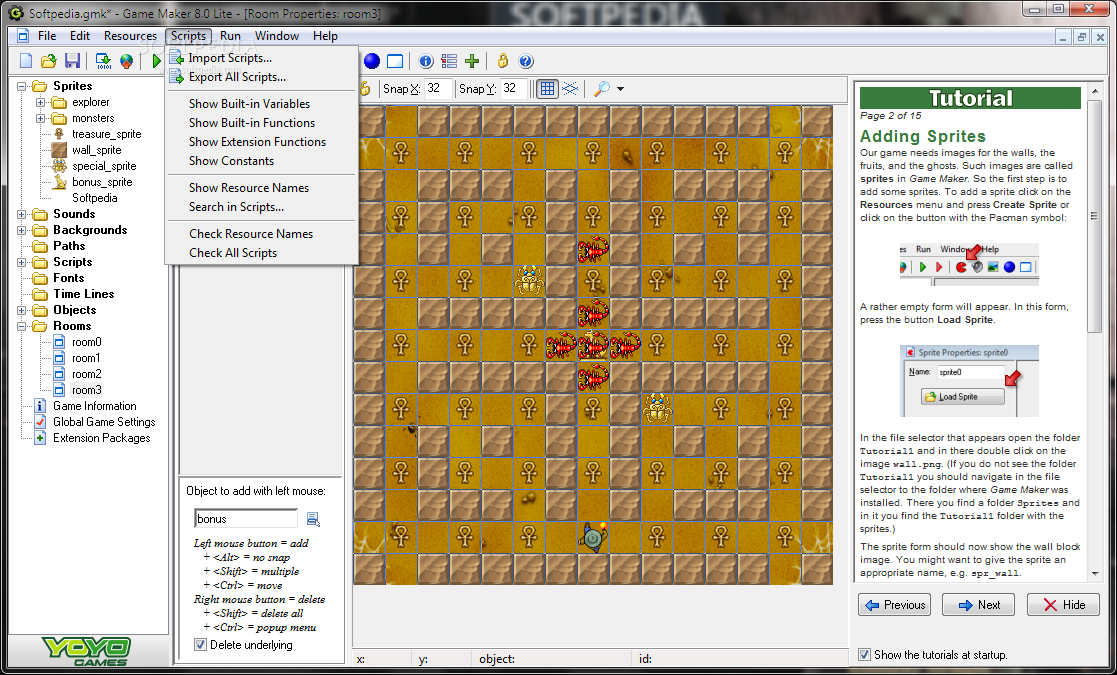
\includegraphics[width=8cm]{Pics/gamemaker1.png}
\end{center}
\caption{Game Maker in action}
\label{fig:game_maker_in_action}
\end{figure}

\subsubsection{Unity 3D}
Unity 3D is an asset-centric game-development system. This means that Unity tries to keep the game developer as much as possible into the visual editor, dragging new game objects into the scene hierarchy, modifying the game objects properties to customize their appearance or behavior along certain predefined ways. The editor also maintains a live preview of the game. Unity 3D supports high quality 3D rendering through support of normal maps, shadows, full-screen post processing, and more.

The underlying architecture is based on components. Components are properties of a game entity that allow a certain entity to follow certain rules. Components may be the ability to follow physics rules, to respond to input commands, and so on. When the developer selects an entity in the editor, he then attaches components to the entity so that it will perform the desired actions.

As in GameMaker, not everything for a moderately complex game can be expressed in a visual editor. Unity supports the execution of custom game scripts via Mono, the open-source implementation of the .NET Framework. Scripts may be written in UnityScript (a custom language inspired by JavaScript), C\#, or the Boo programming language \cite{CHAPTER_3_BOO}.

A screenshot of Unity is shown in Figure \ref{fig:unity_in_action}.

\begin{figure}
\begin{center}
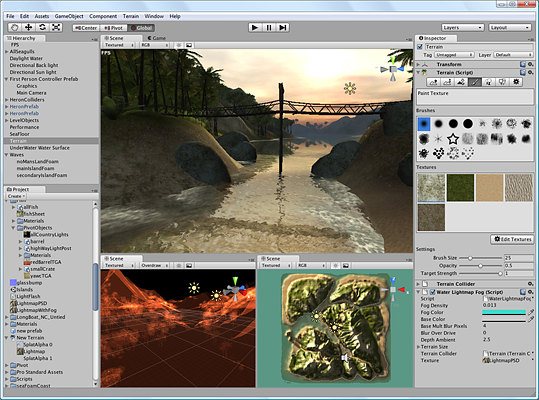
\includegraphics[width=8cm]{Pics/unity1.png}
\end{center}
\caption{Unity in action}
\label{fig:unity_in_action}
\end{figure}

\subsubsection{XNA}
Both GameMaker and Unity pragmatically include a scripting system so that game objects can be manipulated with user-written scripts. These scripts track some logical aspects of the game state, such as score, lives, re-spawning, AIs, etc., and may either be run in response to certain events, or during every tick of the simulation. This may seem in contrast with the visual nature of those editors, which offer many options to create games in a "mostly code-free" fashion. What this ultimately means is that game development is inextricably tied to coding, no matter how powerful visual environments are used. Visual environments can help \textit{reduce} the need to write code, but the number of useful game functions that may be defined is simply so large that expressing it without having to type them in a programming formalism is very hard. For example, consider the number of AI algorithms in existence: state machines, neural networks, fuzzy logic, planning system, genetic algorithms, etc. Furthermore, new algorithms are constantly under study and get published every year. This means that for a game system to support this large amount of algorithms, simply pre-programming all of them is not feasible: they are too many, and new ones are added all the time. 

In short, game development requires coding.

For this reason we also discuss the XNA framework. XNA is a code-centric tool for making games based on the .Net framework. XNA can be used from any .Net language: from C\#, to F\#, to VB.Net. It offers classes that cover most areas of game development. Such classes represent an efficient and easy to use implementation of those small building blocks that are found in virtually all games. XNA starts by supporting the game loop with the \texttt{Game} and \texttt{GameComponent} classes, which manage the creation of the game window, and the invocation of the tick functions of the game loop at the appropriate times. Input is supported by polling the mouse, keyboard, and XBox 360 gamepad. To ease building collision detection and physics, a series of bounding volume classes are supported such as boxes, spheres, planes, etc. that may be checked for intersection with each other. XNA also offers rendering facilities so that the developer can quickly add 2D rendering of alpha-blended sprites and 3D rendering of simple models. Rendering may also use shaders, render targets, and similar advanced features in conjunction with the simple drawing primitives: this makes it possible to create advanced visual effects. Audio is supported with music, positional 3D sounds, and even pre-mixed audio effects created with the XACT audio editor. Networking is, unfortunately, supported only on the XBox with a UDP library that also includes functionality for lobby, friends, invites, and all those features that support some of the more social aspects of multiplayer.

XNA does not offer any visual framework or helper, and instead requires coding all a game, often with a large amount of code.

The XNA "Racing Car Starter Kit" shows the potential of the framework in Figure \ref{fig:xna_in_action}.

\begin{figure}
\begin{center}
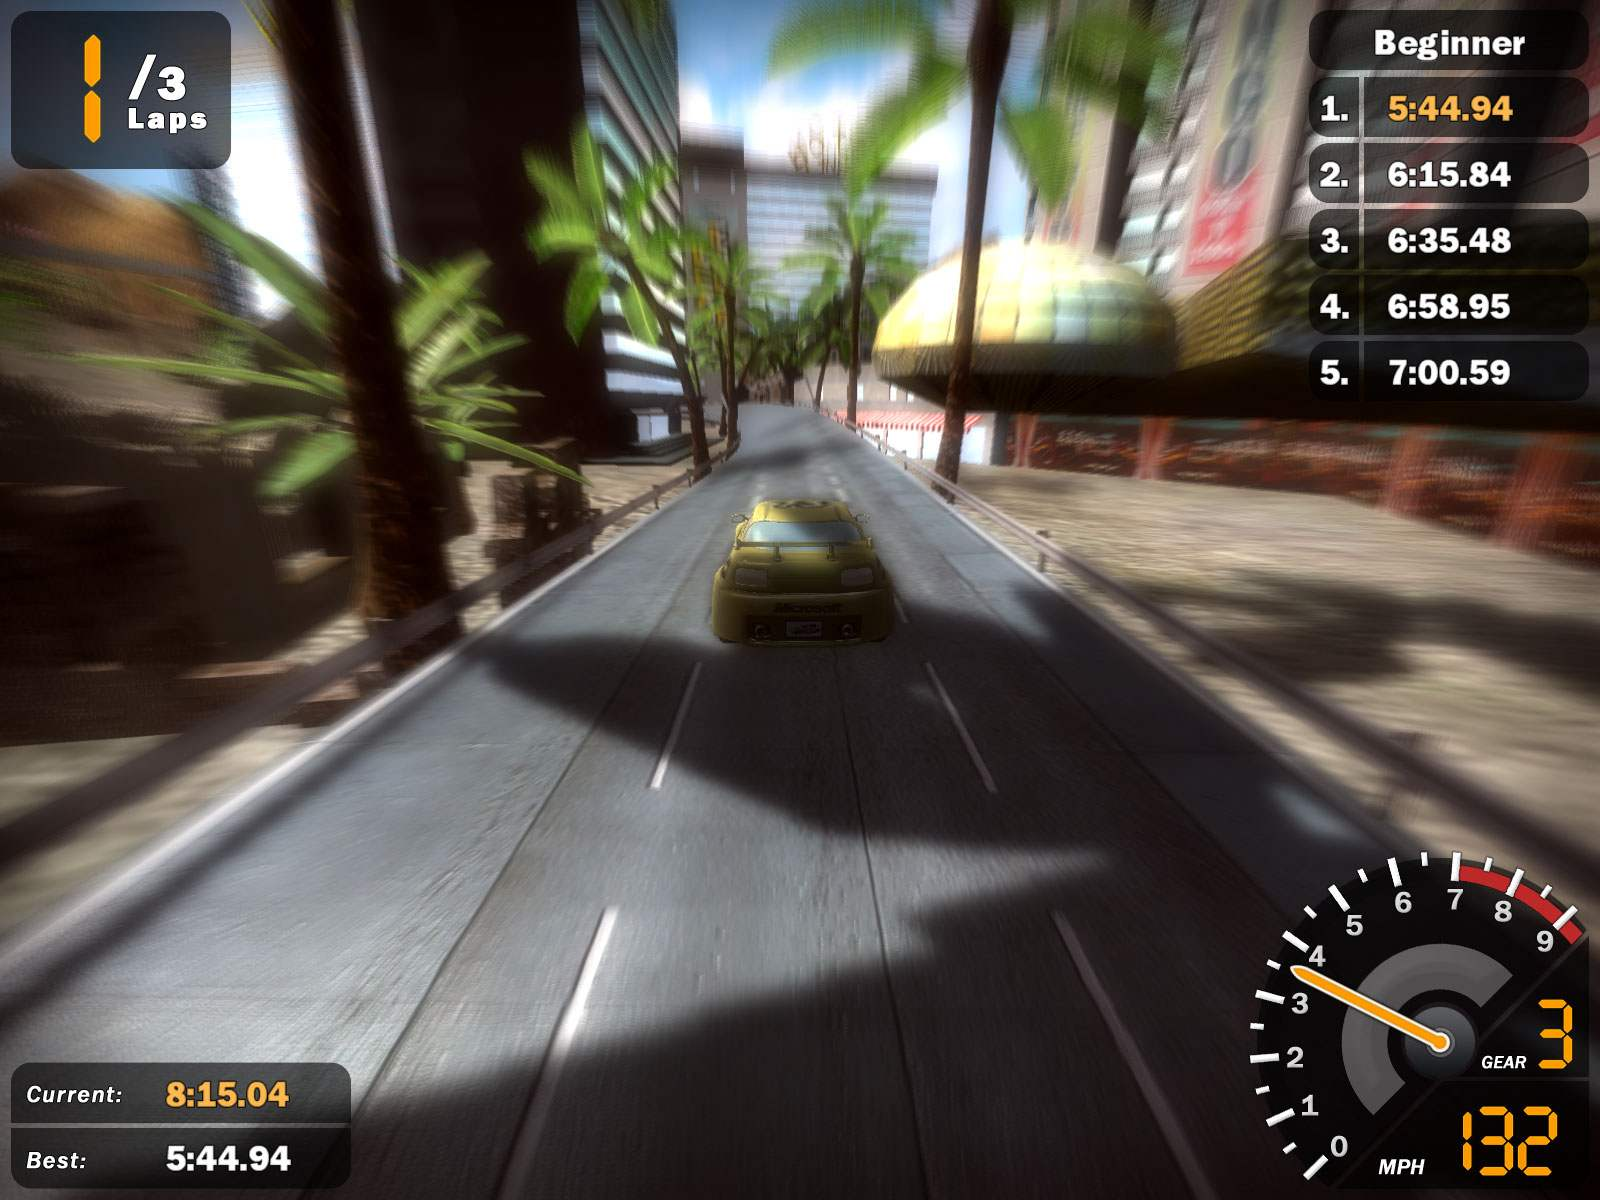
\includegraphics[width=8cm]{Pics/xna1.png}
\end{center}
\caption{XNA in action}
\label{fig:xna_in_action}
\end{figure}


\section{Languages for making games}

Game development can also be done with special-purpose programming languages. Game-development languages are not many, and the possible reasons are multiple: \textit{(i)} building a language is complex and requires specialized knowledge about compilers, parsers, and type-systems, all in addition to knowledge in the specific domain (in our case games) to which the language applies; \textit{(ii)} game development systems compensate their lack of expressive power through the integration of scripting languages; \textit{(iii)} the game development industry is very slow to adopt new programming languages when compared to the IT industry in general, and this has resulted in a very slow progression in the last decades from assembly to C and finally to C++; this is partly due to huge existing code-bases of C/C++ code that is still being used in production, and from the fact that a shift in language would require extensive retraining.

Outside the gaming industry some researchers have experimented with building languages for making games, while the industry mostly focused on libraries for C, C++ or, in later years, C\# as well. The languages built by researchers have all focused on specific aspects of game development, resulting in a very diverse, albeit slightly small, set of specialized languages. The game-specific languages that we will discuss in the following of this chapter are: \textit{(i)} \textit{Simula} \cite{CHAPTER_2_SIMULA67}, an old language built for simulations where many innovations in programming languages were born; \textit{(ii)} \textit{SGL} \cite{SGL}, a recent language from Cornell University which unified the definition of a game loop with a series of heavily optimized SQL-style queries on a global table that stores all the game entities; and \textit{(iii)} \textit{Inform 7} \cite{CHAPTER_2_INFORM}, a programming language which only focuses on a small group of games, that of textual adventures, but allows to write them in plain English instead of a traditional, structured and symbolic programming language.

\subsection{Simula 67}
The first language we discuss is the Simula language, in particular the Simula 67 version (there are two versions: Simula I, and Simula 67, the second being more advanced). Simula is quite an old language, and was one of the precursors of modern object-oriented languages. It was born in 1967, and it focused strongly on building simulations, as the name aptly suggests. In particular, Simula featured objects, inheritance, and a notion of cooperative multi-threading through \textit{coroutines}. Simula ships with a simulation package that allows building discrete event simulations. Simula is also a historically relevant language, in that its object system laid the groundwork for the implementation of objects that is now found in languages such as C++, Java, and C\#. Moreover, Simula made heavy use of coroutines, which are now widely used in modern programming languages to define generators to create collections interactively; coroutines are notably making a comeback in the C\# language in the form of the \texttt{async} and \texttt{await} keywords. Moreover, before \texttt{async} and \texttt{await}, Mono and Unity introduced a customized version of coroutines with the \texttt{yield} statement.

Let us now consider an example of the simulation capabilities of Simula. Sam, Sally, and Andy are shopping for clothes. They have to share one fitting room. Each one of them is browsing the store for about 12 minutes and then uses the fitting room exclusively for about three minutes, each following a normal distribution. A simulation of their fitting room experience is as follows:

\begin{lstlisting}
Simulation Begin 
  Class FittingRoom; Begin 
    Ref (Head) door; 
    Boolean inUse; 
    Procedure request; Begin 
      If inUse Then Begin 
        Wait (door); 
        door.First.Out; 
      End; 
      inUse:= True; 
    End; 
    Procedure leave; Begin 
      inUse:= False; 
      Activate door.First; 
    End; 
    door:- New Head; 
  End;

Procedure report (message); Text message; Begin 
  OutFix (Time, 2, 0); OutText (": " & message); OutImage; 
End;

Process Class Person (pname); Text pname; Begin 
  While True Do Begin 
    Hold (Normal (12, 4, u)); 
    report (pname & " is requesting the fitting room"); 
    fittingroom1.request; 
    report (pname & " has entered the fitting room"); 
    Hold (Normal (3, 1, u)); 
    fittingroom1.leave; 
    report (pname & " has left the fitting room"); 
  End; 
End;

Integer u; 
Ref (FittingRoom) fittingRoom1;

fittingRoom1:- New FittingRoom; 
Activate New Person ("Sam"); 
Activate New Person ("Sally"); 
Activate New Person ("Andy"); 
Hold (100); 
End;
\end{lstlisting}

The \texttt{Simulation} keyword at the beginning of the listing enables the use of simulations. The fitting room object uses a queue called \texttt{door} that arbitrates access to it. If someone requests the fitting room while it is in use, then they must wait in the queue with the \texttt{Wait (door)} statement. When the fitting room is emptied, the first person in the queue is activated with \texttt{Activate door.first} and removed from the queue \texttt{door.First.Out}. A person is modeled as a \texttt{Process} and its activity is described using the \texttt{Hold} statement that suspends the process to simulate browsing the store and being in the fitting room. The person process uses the \texttt{request} and \texttt{leave} methods to obtain and release access to the fitting room.

The main program initializes and activates the various entities of the simulation, which is then run for 100 minutes of simulated time before the program terminates.

Simula pioneered the use of many constructs for building simulations. Even today, programming languages have not managed to achieve the same level of expressive power for simulations that Simula programmers enjoyed. The example above, for instance, would be harder to write in a general-purpose programming language such as C++, given the lack of first-class support for cooperative multi-thread, queues, etc.


\subsection{Inform}
The Inform 7 language is the latest incarnation of Inform, a programming language and design system for interactive fiction originally created in 1993 by Graham Nelson. Inform 7 is a peculiar programming language, in that it addresses a "niche-within-a-niche" of the domain of computer programming. Inform exclusively allows the building of interactive text adventure games, that is those kind of games where the game world is presented to the user with a textual description, and the input that the user gives is, again, with textual commands. This makes Inform's scope \textit{extremely} specific.

The most advanced feature of the Inform programming language is that it allows the programmer to write a game in plain English, albeit with certain grammatical limitations. The language allows the description of the game as a series of objects with properties, together with a series of scenes that the user interacts with. The parsing facilities offered by Inform are indeed very powerful, and they are used to parse the user's input and the programmer's code both expressed in natural language. Inform features a simple object system that allows only for single inheritance and polymorphism; the language is also statically and strongly typed, in order to allow the programmer to reuse some code, but without adding complex notions such as abstraction, so that the concepts that come into play are always as simple as possible. This means that some traditional programming activities are supported by the language, but all constructs are declarative and highly readable.

A sample Inform 7 program could be:

\begin{lstlisting}
"Hello Deductible" by "I.F. Author"

The story headline is "An Interactive Example".

The Living Room is a room. "A comfortably furnished living room." The Kitchen is north of the Living Room. The Front Door is south of the Living Room. The Front Door is a door. The Front Door is closed and locked.

The insurance salesman is a man in the Living Room. "An insurance salesman in a tacky polyester suit. He seems eager to speak to you." Understand "man" as the insurance salesman.

A briefcase is carried by the insurance salesman. The description is "A slightly worn, black briefcase." Understand "case" as the briefcase.

The insurance paperwork is in the briefcase. The description is "Page after page of small legalese." Understand "papers" or "documents" or "forms" as the paperwork.

Instead of listening to the insurance salesman for the first time:

say "The salesman bores you with a discussion of life insurance policies. From his briefcase he pulls some paperwork which he hands to you."; move the insurance paperwork to the player.
\end{lstlisting}

Inform does not feature many of the constructs that would be necessary to build a complex, real-time simulation: there is no notion of a main loop, nor is the language designed to define real-time actions or describe rendering methods besides text. From the point of view of making games \textit{in general} it is woefully under-powered, but when it comes to interactive fiction it is, quite literally, a unique experience to use.

Multiple games have been built with Inform. \textit{Curses}, by Graham Nelson, was the first game ever written in the Inform programming language. \textit{So Far}, by Andrew Plotkin, won the first XYZZY Award for Best Game winner in 1996. \textit{Galatea}, by Emily Short, is considered to have the most complex interaction systems for a non-player character in an interactive fiction game. \textit{Mystery House Possessed}, again by Emily Short, was the first Inform 7 game released to be public. Emily Short's \textit{Floatpoint} won the Interactive Fiction Competition, and the 2006 XYZZY awards for Best Setting and Best NPCs.


\subsection{SGL}
The final language we discuss is the SGL language. SGL, as the name suggests, is a language that descends from the widely known SQL language for expressing declarative queries on databases. 

SGL is based on the idea of defining the game world as a large table of entities, where an entity is a row with a union of all the attributes possible for all entities; all the attributes that are irrelevant to a specific entity are then set to null values. The dynamics of the game, such as physics, damage, grouping, etc. are then defined in terms of a huge query that transforms all entities from one time-step of the simulation into another.

For example, an SGL game could define a unit in a virtual army as:

\begin{lstlisting}
class Unit {
  State:
    number unit_id;
    number player;
    number command;
    number pos_x, pos_y;
    number health;
    Set<number> squad;
  Effects:
    number move_x : AVG;
    number move_y : AVG;
    number damage : SUM;
    Set<number> joined : UNION;
    Set<number> left : UNION;
  Update:
    pos_x = pos_x + move_x;
    pos_y = pos_y + move_y;
    squad = squad UNION joined SETMINUS left;
    health = health - damage;
}	
\end{lstlisting}

The \textit{state} encodes a description of the entity with a set of attributes. The \textit{effects} define a series of queries (similar to Casanova rules) that are further specified as described below. The \textit{update} specifies how the state of the entity changes at every tick of the game loop.

Queries that move units towards enemy clusters may be defined with SQL-style aggregations such as:

\begin{lstlisting}
let enemies = (all u in Units where u.player != me.player);
let centroid_x = AVG(enemies.x_pos);
let centroid_y = AVG(enemies.y_pos);
let me.move_x = (me.pos_x - closest.pos_x)/norm;
let me.move_y = (me.pos_y - closest.pos_y)/norm;
\end{lstlisting}

SGL games retain most of the readability of SQL queries, that is, even though an SGL game will not be as simple and pleasant to read as an Inform code listing (few programming languages can boast such feature), it is still far simpler to read than equivalent low-level code. The high-level semantics at which SGL games are expressed allows the SGL engine to know more about what computations the game performs; SGL, for example, will be able to understand that we wish to compute a certain Cartesian product between certain lists, and it will be able to automatically create a support index to turn the evaluation of this product from the $O(n^2)$ complexity of the naïve implementation into the much lower $O(n \log n)$ of a balanced search tree. The complex algorithmic optimizations made by SGL are usually done by hand in traditional game development (often many times in the same game) by developers, and with lots of effort. In this sense SGL allows a developer to create a game without worrying about performance but obtaining the run-time performance that results from the use of hand-written, specialized, complex algorithms.

SGL also assumes the presence of other game engine modules such as a rendering module, an input module, and even pathfinding facilities. From this point of view SGL is not a fully-fledged game programming language, but it allows building efficiently the core module of a modern game.


\section{Motivating a new programming language}
Creating a new programming language may be seen as a fruitless endeavor. Specifically, there are many programming languages that have been created as part of research efforts. Very rarely such languages have seen widespread adoption, and virtually all of them have been confined to research labs.

It should be noticed that the purpose of such research has never been that of creating industrial-grade tools that are used by many. Rather, the purpose of programming languages research is to shed new light on the best practices by exploring \textit{unknown possibilities} \cite{CHAPTER_1_PL_RESEARCH}. Indeed, many defunct research languages actually paved the way for innovations in future languages \cite{CHAPTER_1_PL_INFLUENCE_ON_PL} and even tools and systems that are now wide-spread (for a recent example, see \cite{CHAPTER_1_PL_INFLUENCE_ON_CURRENT_LANGUAGES}). Also, programming language research has often automated lessons from the field of Software Engineering, as described in \cite{CHAPTER_1_PL_AND_SWENG}.
Sometimes there have even been decades of difference in terms of time between invention and adoption. One need only realize that research in programming languages has yielded benefits that range from sub-routines \cite{CHAPTER_1_PL_SUBROUTINES}, to data structures \cite{CHAPTER_1_PL_DATASTRUCTURES}, to objects \cite{CHAPTER_1_PL_OBJECTS}, to delegates and callbacks \cite{CHAPTER_1_PL_HOF}, to generics \cite{CHAPTER_1_PL_INFLUENCE_ON_PL}, to compile-time meta-programming \cite{CHAPTER_1_PL_GENERIC_PROGRAMMING}, to garbage collection \cite{CHAPTER_1_PL_GARBAGE_COLLECTION}, and so on.

The motivation for choosing to create a programming language rather than trying to engineer (yet another) game development system, is also grounded in the observation that there exist many game development systems. From top-of-the-line game engines such as ID's engines, CryTek, Aurora, etc. to simpler tools aimed at hobbyist or indie developers such as Unity, GameMaker, XNA, and others, most existing systems either fall short in generality (it is rare that an FPS engine works well for other genres, such as RTSes, and vice-versa), they fall short in expressive power, or the do not offer a significant advantage to developer besides a few handy facilities.

Additionally, as game development tools and systems are a heavily explored field, we argue that designing a language for making games is a welcome departure from traditional approaches, and it may lead to novel insights and understanding in the field.

it is a possible source of novel insight to study how the problem of game development can be tackled by language design.

In general, building a programming language offers relevant advantages over designing a system. Ever since the dawn of computer science, programming languages have flourished. Despite Church and Turing's insights that all programming languages are born equal, new programming languages keep on being invented, each with its own strengths and weaknesses. 

In the following we explore some of the strengths afforded to programming language designers. We do not claim that the list of items discussed below is complete, nor do we claim that it is our own invention and discovery. What follows is distilled from a survey of the literature, with particular focus on seminal works such as \cite{CHAPTER_1_PL_OBJECTS, CHAPTER_1_CODE_MANAGEMENT, CHAPTER_1_PL_INFLUENCE_ON_PL, CHAPTER_1_PL_TYPE_SYSTEMS_AND_MEMORY_ALIGNMENT, CHAPTER_1_PL_AND_SWENG, CHAPTER_1_TESTING_DOES_NOT_WORK}, as highlighted by our our own experience. From this, we observe that languages are primarily: \textit{(i)} syntactic abstraction mechanisms that reduce repetitive code; \textit{(ii)} thought shapers that induce a paradigm shift in how one should structure software; \textit{(iii)} simplifiers that boil down an existing paradigm to just its essential parts, often to increase understanding and insight; \textit{(iv)} law enforcers that make sure important invariants hold, to increase correctness, performance, or other properties. 

We now discuss how a programming language affects the \textit{(i)} flexibility, \textit{(ii)}  correctness, and \textit{(iii)} efficiency of the programs written in it. We describe why and how each of these three aspects is important for games and briefly note the relevance of each item with respect to game-development. We also explain how game development systems and languages fare in that regard.

\subsection{Flexibility}
Software is flexible when it is \textit{easy to understand, modify, and extend}. This is achieved through structuring the program well, but a programming language can help with the structuring.

Games are modified and tuned up to the very end of their development cycle, and sometimes even beyond \cite{CHAPTER_1_PATCHING_CYCLES}. This means that flexible architectures for making games are of importance for game developers.

Game development systems are usually designed with a series of predefined scenarios in mind, and depending on the system it may well be impossible to push it beyond its originally intended boundaries, even if it is sometimes needed. This makes such systems not truly flexible.

Flexibility depends on abstraction \cite{CHAPTER_1_CODE_MANAGEMENT,CHAPTER_1_PL_INFLUENCE_ON_PL}, which allows to reuse code and define general solutions that can be reused across similar problems that arise multiple times.

\subsubsection{Abstraction}
The ability to create hierarchies of libraries makes it possible for a developer to capitalize on the work done by others before him. Programming languages allow the definition of \textit{reusable units}: procedures and functions allow avoiding duplicating code, data abstraction allows to reuse "similar" but otherwise different data-types in the same context without rewriting the same operation many times, and entire modules can be abstracted with design patterns.

Games feature huge code bases \cite{CHAPTER_1_SIZE_OF_GAMES} that we argue could be greatly reduced in size if some forms of abstraction were used to avoid re-writing large similar parts. Game engines are a relevant example of this process in action.

Abstraction is impossible (or much harder to achieve) with systems where the user only has a GUI to perform actions. This happens because even though action sequences can be recorded, it is hard to make the recorded sequence \textit{parametric} so that with a simple change in some parameter then we obtain a different (but similar) sequence of actions.

\subsection{Correctness}
Software is always supposed to achieve a certain task under certain \textit{requirements of correctness}. Programming languages can help establish certain degrees of correctness by offering ways to specify and check important properties \cite{CHAPTER_1_PL_STATIC_ANALYSIS}.

In game development, correctness constraints could be specified so that, for example, the language ensures the correct dimensional analysis for physics quantities, the correct generation of state machines, etc.

Systems that are well-designed and well-tested often offer strong correctness guarantees, since they force the user to interact with the project only according to a predefined set of rules and by sanitizing his input so that only safe operations are performed.

Correctness depends on: \textit{(i)} memory safety to ensure that the program does not manipulate nonsensical values; \textit{(ii)} concurrency control to arbitrate accesses to shared resources; and \textit{(iii)} testing to find bugs, or exclude them to a certain degree.

\subsubsection{Memory Safety}
Accessing unallocated memory, jumping to data-addresses, or in general \textit{carelessly manipulating memory addresses} can result in catastrophic, hard to debug errors. By using a static type-system that ensures that all data manipulated and passed to procedures is of the correct type ensures that memory accesses are always properly aligned \cite{CHAPTER_1_PL_TYPE_SYSTEMS_AND_MEMORY_ALIGNMENT}. Static type systems have no run-time overhead, that is after the program is type-checked at compile time the produced assembly code has no trace of the types used during compilation. Garbage collection also helps ensuring such safety \cite{CHAPTER_1_PL_GARBAGE_COLLECTION}.

Games manage large numbers of objects with unpredictable, highly dynamic lifetimes. This makes a reliable memory system useful because thanks to it the developer does not have to manually track the life-cycle of an entity to deallocate its representation by hand; such a technique risks to maintain references to a deallocated entity, or to not deallocate some entities that are not references anymore and which thus occupy memory for no reason.

Game systems achieve correctness through extensive testing \cite{CHAPTER_1_PATCHING_CYCLES}, and often make use of unsafe memory manipulation techniques \cite{CHAPTER_1_POINTER_ARITHMETICS_IN_GAME}. As such, they only offer empirical guarantees (through extensive testing \cite{CHAPTER_1_TESTING_DOES_NOT_WORK}) about the memory safety of games, and moreover they never exclude the possibility of memory leaks or similar mishaps since running the game may encounter conditions which did not occur during testing.

\subsubsection{Concurrency Control}
Languages often operate on shared resources accessed by \textit{concurrent processes}.

This is particularly relevant in a game, where many entities operate concurrently on the game world \cite{CHAPTER_1_GAMES_ARE_CONCURRENT}, and they must be synchronized in order to guarantee that the logical invariants of the game are respected.

A system can have a predefined, monolithic system for managing concurrency, while a language can define a paradigm that (to various degrees) arbitrates access to shared resources \cite{CHAPTER_1_PL_AND_RESOURCE_SHARING}.

\subsubsection{Bug finding}
Most software development is spent on \textit{testing}, rather than writing code \cite{CHAPTER_1_TESTING_MORE_THAN_WRITING}. By forcing certain properties on a program (or on parts of it), such as the absence of side-effects in functions, it becomes easier to test a program in a bottom-up fashion. The absence of side-effects allows testing smaller pieces of the program in isolation first, and then testing their composition until most of the program is tested properly. In contrast, programs where many functions read and write on lots of global values requires testing one's program against all combinations of function call sequences and initial values of the shared state: such a task may be nigh impossible.

The number of possible configurations in a game world is very large, given that many entities in the game can move, change their internal statistics, etc. The very large space that must be tested in games allows them to benefit significantly from a bottom-up testing strategy in the absence of side effects, since this would reduce the number of tests to be performed while being assured that composing the smaller parts of the game that have been tested preserves correctness.

Game systems usually allow the definition and concurrent manipulation of global game variables, and in general suffer the issue where the insertion in the game of an apparently innocent and (locally) correct procedure may suddenly break something else (which may even appear to be unrelated).

\subsection{Efficiency}
Software efficiency is measured by the amount of resources it uses to accomplish its task. A variety of resources can be considered, from time and space to network bandwidth, power, and databases. When \textit{resources are constrained}, a language' constructs and compiler can be made aware of these resources and even of the possible optimization strategies \cite{CHAPTER_1_COMPILER_OPTIMIZATIONS}. A language can make it easier to express efficient algorithms by supporting efficient data structure declaration and traversal; for example, we can observe that building a balanced binary tree is simpler \footnote{Or at least much closer to its definition in mathematical notation, and relatively far from the technical details of a computer.} to do with union types (see Appendix \ref{chap:fsharp}) in the style of ML rather than with C structures and pointers. A compiler or interpreter such as those used for SQL can also heavily elaborate the input program and insert the appropriate optimizations so that the user does not have to do so by hand (and sometimes without even being aware of them) and still get an efficient program \cite{DATABASE_SYSTEM_IMPLEMENTATION}.

In game development CPU time is a crucial resource, since if the game runs slowly then the gaming experience will fail to be immersive and the game will have missed its mark. A language that is aware of the needs of a game can help by ensuring that any code written for the game will be optimized automatically, for example running certain portions of the game logic in parallel or optimizing Cartesian products with the use of spatial partitioning indices.

Game development systems usually provide a series of commonly used underlying services such as rendering, input management, and physics, which are highly optimized; they then rely on the game developer to not write code that will slow down the game excessively.


\section{Creating new languages for making games}
As a conclusion, we note that game development, even with the most advanced systems, still requires a significant amount of programming. Unfortunately, this is not done with special-purpose programming languages; such languages would yield significant benefits (as discussed in the previous section) to game developers, and such benefits are currently ignored completely by game development companies. Moreover, game development systems have shortcomings which are often just worked around by game developers, as outlined in the comparison of Table \ref{tab:systems vs languages}. Therefore, from the next chapter on we will introduce the Casanova language, designed exclusively for making games. Our objective is not that of designing and building \textit{the} ultimate game development language. Our aim is less ambitious: we will simply show the benefits of adopting \textit{a} game development language, as long as it is properly designed.

\begin{table} 
\center
\begin{tabular}{ | p{7cm} | p{7cm} |}

\hline
Systems & Languages \\
\hline

easier to use from the start & harder to use from the start \\ & \\

leverage existing technical knowledge & obtain new knowledge \\ & \\

write small amounts of code & write large amounts of code \\ & \\

leverage high quality components done by others & leverage high quality components done by others \\ & \\

obtain good results with little effort right away & obtain good results with little effort after the learning phase \\ & \\

games from a system look similar to one another & games can vary a lot between one another \\ & \\

expressive power is limited & expressive power is absolute \\ & \\

complex tasks that are not pre-built have no support or even awkward support & all complex tasks are supported \\

\hline

\end{tabular}
\caption{Systems vs languages}
\label{tab:systems vs languages}
\end{table}


\begin{comment}
One aspect that emerges from the analysis of game development systems and languages is that coding is an ubiquitous activity that cannot be marginalized or outright removed from game development. Nevertheless, smartly designed visual editors that access well-written libraries can save a good deal of development effort by allowing the developer to drag-and-drop to place objects and activate their properties; after this phase, scripts of code are written as needed, to realize more complex behaviors that are not supported by the underlying libraries. This means that even the best designed systems can benefit from powerful languages for game development. We argue that the use of game development languages that are built for general-purpose use is inappropriate, since the features of these languages often are incompatible with the needs of the game.

We believe that one final detail is worthy of notice. All visual editors require, at some point, the use of a programming language to express some of the most complex custom aspects of a game. This means that their difficulty curve is at most as high as that of their languages, even if novices that do not (yet) write code for their game may not notice it in the beginning, thus giving the impression of an easier to use system. As such, visual editors simply postpone as much as they can the difficulties of learning how to program for games, and they automate some common game programming activities, but they do not eliminate the need for coding.
\end{comment}
 

\chapter{Design of Casanova}
\footnotetext{This chapter is partially derived from the paper \cite{CASANOVA_ACG}.}
\label{chap:design}
In this chapter we describe the informal design of Casanova, that is how Casanova came to be in its current shape. We start by describing our realization of a fundamental design pattern that kept recurring in games, which we called \textit{rule-script-draw} (or RSD in short). We then state the reason why we decided to build a whole new language instead of trying to capture RSD in an object-oriented library, as is often down for design patterns. We then give our design goals, which is a statement of the overall objective that we prefix ourselves with for Casanova. We conclude the chapter with an informal presentation of the Casanova language.


\section{The RSD pattern}
RSD is a game development concept which captures the definition of a game completely. Through our direct experience in game development, and through a survey of the informal (such as blogs, websites, and discussion boards) and formal literature of game making, we have come to the realization that game development always touches upon some fundamental concepts. These are the three main components of games, and their interactions.

The game is made up of its game logic, and its drawing. The game logic is, in turn, made up of \textit{regular} aspects of the game, such as physics equations and other continuous parts of the numerical integration of the game, and \textit{irregular} aspects of the game, such as timers, AI, state machines and other discrete parts of the numerical integration of the game. Finally, many aspects of the logic are \textit{drawn} to the screen for the user to see. These three aspects are the cornerstones of the RSD pattern:

\begin{itemize}
\item \textit{rules}, the regular aspects of the game logic
\item \textit{scripts}, the irregular aspects of the game logic
\item \textit{drawing}, the drawing of the game to screen
\end{itemize}

Unfortunately, most games are built without explicit awareness of these components. This means that efforts to capture these so that building new games in them requires less time and expenditure of resources are not well focused if they do not consider such aspects. For example, frameworks such as XNA or DirectX UT offer (limited) support to rules and drawing, but no support whatsoever to scripts. More advanced systems such as Unity, on the other hand, offer further support for scripts through coroutines. 

Development of Casanova started as an effort towards capturing the RSD pattern. We started by trying to build a library in the usual spirit of design patterns, but ended realizing a language when we understood that a library would not be sufficiently pervasive to capture all we needed.
 
We observe that some work has been made towards identifying recurring patterns in game development, for example \cite{bjork2005patterns, stoy2006components}, but these efforts often take for granted some underlying basic patterns (such as RSD) that they rely upon, and offer highly articulated (and often complex) solutions. These patterns require large amounts of focus on the part of the developer, who is required to perform the functions of a ``human compiler''. We believe that complex design patterns such as those cited above are often an indication of language issues \cite{Sullivan02advancedprogramming}, and they reinforce our belief in the need for a specific game development language.


\section{Motivation for a new language}
RSD is a very abstract design pattern that is hard to represent because of its high-granularity. Capturing it with mainstream tools such as an object-oriented library proved hard. For example, defining how to evaluate rules over fields of data-structures requires induction over the fields themselves, and access to their type. Such meta-programming constructs are not readily available in commonly used programming languages such as C\# or C++, and when they are their use is unfortunately quite awkward (see Appendix \ref{chap:casanova_in_haskell_and_cpp}). Moreover, using tools such as inheritance also gave us trouble because of an excessive number of virtual calls, which disrupts performance in a way that results incompatible with game development.

For this reason, we decided to pursue the definition of a whole new language, in order to be free from the representation and performance constraints given by existing languages. We believe that such a language, in addition to faithfully representing the RSD pattern, must offer two fundamental features. On one hand, the language must be flexible enough so that a developer can use it effectively to build \textit{any} kind of game or simulation. The language should never lose expressive power, even when tackling scenarios that were not directly foreseen by its developers. On the other hand, the language must be optimized for the domain of games and simulations. It should not require the developer to specify too many details. Specifically, the language should require from the developer only the relevant details for the game. The language compiler and its run-time facilities should then fill in the blanks by adding all the additional boilerplate code that takes care of the various needs of the game. The developer should not focus his efforts on the game loop, reading input, hand-crafting state machines, and other menial tasks; this does not diminish the role of the developer at all: instead, it frees him to pursue other tasks that are more complex and interesting, such as building a better game logic, modeling AIs with stronger algorithms, applying procedural generation to levels and stories, and so on. There really are no boundaries to the complexity of a game or a simulation, so the more powerful the tools the more difficult goals may become achievable.


\section{Design Goals}
We sum up the targets that we have for the design of Casanova in the following table. These targets describe both the requirements of the RSD pattern, and also additional requirements about the expressive power and simplicity of the language.

\begin{tabular}{ | l | p{9cm} | }
\hline
1. & Allow a developer to build games without explicit limitations in terms of genre or creativity \\
\hline
2. & Support common game development tasks of handling the game logic, game AIs, state machines, drawing, and input \\
\hline
3. & Be concise, in particular when compared with traditional programming languages used for the same games \\
\hline
4. & Be efficient, supporting fast runtime execution of the game and common optimizations such as multi-threading or query optimizations \\
\hline
5. & Be simple to read, supporting syntactic idioms that are grounded in logic and mathematics rather than aping the syntax of widespread programming languages \\
\hline
6. & Contain as few features as possible, that is the language should be built on top of few orthogonal \cite{CHAPTER_4_ORTHOGONALITY_PL} constructs that each serve a clear purpose and that mix well together \\
\hline
\end{tabular} 

These goals, if fulfilled, will result in a simple, expressive, and efficient language that is suitable for creating games and simulations. We will refer to these goals in the final evaluation of the language.


\section{Informal design}

Casanova models a game by defining: \textit{(i)} the \textit{model of the world}, that is what entities and values we track to represent the game world; \textit{(ii)} the physical and logical \textit{rules} that the game entities obey; \textit{(iii)} the \textit{state machines} that handle irregular game logic that would be difficult to express in terms of game rules; \textit{(iv)} the \textit{visual appearance} of the game entities; and \textit{(v)} the \textit{initial state} of the world when the game is launched. 

As an example, let us consider a very simple pseudo-game that simulates a bunch of bouncing balls. We will use a pseudo-Casanova language before diving into the proper syntax. The model for our game world will simply define the world as:

\begin{lstlisting}
World = a series of balls
\end{lstlisting}

A ball would then be defined as:

\begin{lstlisting}
Ball = 
  current position of the ball
  current velocity of the ball
  a picture of a ball
\end{lstlisting}

We now define the logical and physical rules of the world and its entities, that is we specify how each entity updates its fields. The rules for the world state that:

\begin{lstlisting}
World rules = 
  when a ball exits the screen then it is not considered anymore in the state
\end{lstlisting}

The rules for the ball are slightly more complex, since we have to simulate some simple bouncing physics and we also have to update the sprite data:

\begin{lstlisting}
Ball rules =
  the position is the numerical integration of the velocity
  the velocity is the numerical integration of gravity, but when the position touches the ground then the velocity is turned upside-down
  the sprite position is the same as the ball position
\end{lstlisting}

With the information provided above we now have a simplistic simulation that runs by updating some bouncing balls which are then "forgotten" from the game state whenever they leave the screen. We wish the simulation to be made marginally more interesting, and to achieve this result we will spawn balls automatically so that there is an endless supply of moving things on the screen. We model this behavior with a script:

\begin{lstlisting}
wait between one and three seconds
add to the world a random ball
repeat
\end{lstlisting}

Finally, we define the initial state of the world, that is what happens when the world is first activated as the game is launched:

\begin{lstlisting}
Initial world = 
  an empty collection of balls
\end{lstlisting}

As we can see, the above description of the balls game is clear and simple, but we are not leaving behind any important details about what the game will do. Compared with a traditional game development library, though, there is no mention of the game loop, neither for updating the world nor for rendering, and drawing is implicit in the presence of an appearance inside the ball definition; also, the creation of new balls is defined as a simple, sequential process where the various operations are expressed in a top-down sequence instead of a traditional state machine. Also notice that we are not assuming the presence of prefabricated entities to have physics or timed operations, that is we have described everything ourselves.

In the following we will describe how the Casanova language is defined to make it possible to express the above logic in an equally simple and straightforward manner, and how this description is turned into an actual, executable specification for a fast-enough game.
 

\chapter{Syntax of Casanova}
\footnotetext{This chapter is partially derived from the paper \cite{CASANOVA_ACG}.}
\label{chap:syntax}
In this chapter we give the syntax of the Casanova language. The syntax of the language is an abstract definition of all the valid strings that are part of the language. The most common tool to give the syntax of a language is, of course, a formal grammar. Since Casanova is a statically typed language, the grammar is insufficient to capture all the valid programs. Some programs for which typing is incorrect would be accepted by the grammar, but would not be valid Casanova programs. For example, consider the following simple expression:

\begin{lstlisting}
if a < b then 0 else "zero"
\end{lstlisting}

The expression above can be generated by the grammar of Casanova, but it would be rejected by its type system since it is not possible to unify the types \texttt{int} and \texttt{string} of the two branches. To give the full syntax of Casanova we must also know the typing rules, which in fact we give together with the grammar.

\section{Grammar}
The grammar of Casanova states that a valid program starts with a series of mutually recursive \textit{type definitions}; mutual recursion means that the definition of a type may use any other type defined in the program, regardless of the fact that the referenced type definition happens after the definition of the current type. 

Type definitions also contain \textit{rules}, which are special methods that cannot be used by the developer explicitly, but only by the framework; rules are associated with exactly one attribute, and one attribute may be associated to at most one rule. Rules define declaratively what the value for an attribute will be at the next iteration of the game loop, and a rule can access the previous values of the game world and the entity of which it is performing a partial update. Rules cannot have side-effects beyond their implicit one, that is a rule is not allowed to write variables or modify anything. Its only side-effect comes from the fact that its result will become part of the game world at the next iteration of the game loop. 

The program then contains a definition of the \textit{initial value} of the game world. 

Finally, the program must have a \textit{main script} that defines the process that will handle the high-level game logic, plus a series of \textit{input scripts}. All scripts are defined through coroutines.

The grammar that describes the syntax of a Casanova program then is:

\begin{lstlisting}[texcl]
<p>          ::= <type-decls> <initial-world> <scripts>
<type-decls> ::= <type-decl> | <type-decl> <type-decls>
<type-decl>  ::= `type' <id> `=' <type-body>
<type-body>  ::= <record-body> | <union-body>

<record-body> ::= `{' <labels> `}' <rules>
<labels>      ::= <label> | <label>`;' <labels>
<label>       ::= <id> `:' <type-expr>

<type-expr>           ::= <id> | <tuple-type-expr> 
                        | <intrinsic-type-expr>
<tuple-type-expr>     ::= <type-expr> 
                        | <type-expr> `*' <tuple-type-expr>
<intrinsic-type-expr> ::= `Var<'<type-expr>`>' 
                        | `Ref<'<type-expr>`>' 
                        | `List<'<type-expr>`>' 
                        | `Coroutine<'<type-expr>`>' 
                        | float | int | Vector2 | ...
<rules>               ::= empty | <rule> <rules>
<rule>                ::= `rule' <rule-id> `=' <expr>
<rule-id>             ::= <id> | <id>`.'<rule-id>
<union-body>          ::= <id> | <id> `of' <type-expr> 
                        | <id> `|' <union-body> 
                        | <id> `of' <type-expr> `|' <union-body>

<type-init>           ::= <tuple-init> | <list-init> 
                        | <record-init> | <union-init> 
                        | <intrinsic-type-init>
<tuple-init>          ::= <expr> | <expr>, <tuple-init>
<list-init>           ::= `[' <expr-list> `]' | `[' <list-compr> `]'
<list-compr>          ::= `for' <id> `in' <expr> `do' <expr>
<expr-list>           ::= `' | <expr> `;' <expr-list>
<record-init>         ::= `{' <labels-init> `}'
<labels-init>         ::= <id> `=' <expr> | <id> `=' <expr> `;' <labels-init>
<union-init>          ::= <id> | <id> <tuple-init>
<intrinsic-type-init> ::= `ref' <expr> | `var' <expr> 
                        | `Vector2(' <expr> `,' <expr> `)' | ...
<type-dest>           ::= `let' <ids> `=' <expr> | <match-case> 
                        | <match-list> | <id> `.' <id>
<ids>                 ::= <id> | <id> `,' <ids>
<match-case>          ::= `match' <expr> `with' <patterns>
<patterns>            ::= <pattern> | <pattern> `|' <patterns>
<pattern>             ::= <id> | <ids> | <id> `(' <pattern-args> `)'
<pattern-args>        ::= <pattern-arg> | <pattern-arg> `,' <pattern-args>
<pattern-arg>         ::= <id> | <const>
<match-list>          ::= `[]' | <id> `::' <id>

<id-decl> ::= <id> | <id> `:' <type-expr>
<expr>    ::= <id> | <const> 
            | `let' <id> `=' <expr> `in' <expr> 
            | `if' <expr> `then' <expr> `else' <expr> 
            | <type-init> | <type-dest> 
            | <co-expr> | ...
<co-expr> ::= `co{' <co-expr> `}' | <expr> | `return' <expr> 
            | `let!' <id> `=' <expr> `in' <expr> 
            | `do!' <expr> `;' <expr> 
            | <expr> `||' <expr> | <expr> `&&' <expr> 
            | <expr> `=>' <expr> | `repeat' <expr> 
            | `yield'
<id>      ::= ... (* an alphanumeric string *)
<const>   ::= ... (* a constant value *)

<initial-world> ::= `let world =' <expr>
<scripts>       ::= <main-script> <input-script> 
<main-script>   ::= `let main =' <expr>
<input-script>  ::= `let input =' <expr>
\end{lstlisting}

We have omitted some of the grammatical structures which are best known from the literature (see, for one example, \cite{CHAPTER_1_PL_INFLUENCE_ON_PL}): \textit{(i)} the full list of supported intrinsic types (strings, matrices, 3D and 4D vectors, etc.); \textit{(ii)} the initialization syntax for the intrinsic types; and \textit{(iii)} expressions may assume a very large number of shapes, from arithmetic operations such as \textit{expr + expr}, to function calls, function definitions, library functions such as \texttt{List.length}, etc.

\section{Type System}
The type system for Casanova contains the standard functional type system of F\#; this means that we have the usual rules such as:

\begin{mathpar}

\inferrule
{\Gamma \vdash t_1:\texttt{U,}\ \Gamma,x:\texttt{U} \vdash t_2:\texttt{V}}
{\Gamma \vdash \texttt{let }x \texttt{=} t_1 \texttt{ in } t_2:V}

\inferrule
{\Gamma \vdash cond:\texttt{bool}, t_1:\texttt{U}, t_2:\texttt{U}}
{\Gamma \vdash \texttt{if }cond\texttt{ then }t_1\texttt{ else } t_2:U}

\inferrule
{\Gamma \vdash f:U \rightarrow V, t:U}
{\Gamma \vdash f t:V}

\inferrule
{\Gamma \vdash t:\{l_1:T_1;l_2:T_2;...l_n:T_n\}}
{\Gamma \vdash t.l_i:T_i}
\end{mathpar}

and so on. For a complete treatment of the rules of a programming language with this kind of this type system, there are many excellent sources such as \cite{CHAPTER_1_PL_INFLUENCE_ON_PL}.

The most unusual and novel aspects of Casanova's type system are two: rules, and coroutines. We are now going to explain them in detail. 

\subsection{Rules}
Rules are functions that take as input the game world, the current entity the rule belongs to, and the delta time since the last evaluation of this rule; the rule type has range equal to the type identified by its name, treated as a record label. A rule is well-defined if the following holds for all rules:

\begin{lstlisting}
type ID = { l1:T1; l2:T2; ... ln:Tn } 
  rule li = (ei:World * ID * float<s> -> Ti)
\end{lstlisting}

For example we could write:

\begin{lstlisting}
type Ball = { P:Vector2<m>; V:Vector2<m/s> } 
  rule P(world:World,self:Ball,dt:float<s>) =
    self.P + self.V * dt
\end{lstlisting}

We could also write the very same definition where the method body is defined as a function value as:

\begin{lstlisting}
type Ball = { P:Vector2<m>; V:Vector2<m/s> } 
  rule P = fun (world:World,self:Ball,dt:float<s>) ->
    self.P + self.V * dt
\end{lstlisting}

Rules may also refer to the fields inside the value of an attribute. For example, a rule may define how attribute \texttt{kj} of attribute \texttt{li} is updated as in the following:

\begin{lstlisting}
type ID = { l1:T1; ...; li:{k1:V1; k2:V2; ... km:Vm} ln:Tn } 
  rule li.kj = (eij:World * ID * float<s> -> Vj)
\end{lstlisting}

For example we could only update the \texttt{Y} field of the ball position as:

\begin{lstlisting}
type Ball = { P:Vector2<m>; VelY:float<m/s> } 
  rule P.Y(world:World,self:Ball,dt:float<s>) =
    self.P.Y + self.VelY * dt
\end{lstlisting}


Longer chains are handled in a similar fashion.

\subsection{Coroutines}
The second novel aspect of Casanova is that it uses a rare \footnote{rare in applied work on programming languages as compared to theoretical research} feature of type systems that assigns a type to mutable computations. Mutable computations are all those statements that have side-effects such as modifying the memory through an assignment, sending data across the network, drawing to the screen, etc. For this reason mutable computations are also referred to as \textit{effectful}. For example, in a traditional imperative language such as C, Java or others, assigning a variable is just a statement with type \texttt{void}. The same holds true for F\# as well, which types these effectful computations as \texttt{Unit}, which behaves essentially like \texttt{void}. In Casanova, on the other hand, effectful computations are all typed in terms of \textit{coroutines} in order to clearly delimit their usage. For example, assignment has type:

\begin{mathpar}
\inferrule
{\Gamma \vdash t_1:\texttt{var<T>},t_2:\texttt{T}}
{\Gamma \vdash t_1:=t_2:\texttt{Co<Unit>}}
\end{mathpar}

\noindent{where} we used the \texttt{Co} abbreviation for \texttt{Coroutine}. Reading a variable, on the other hand, does not cause any side-effects and so it is not typed in terms of coroutines:

\begin{mathpar}
\inferrule
{\Gamma \vdash t:\texttt{Var<T>}}
{\Gamma \vdash !t:\texttt{T}}
\end{mathpar}

The main point of coroutines is that they are the only place where the developer can put all the side-effects he needs, in a "safe place" where those side effects will not interact in undesired ways between each other. Containing side-effects enables us to safely perform optimizations that would otherwise be impossible because side-effects would break the invariants needed for such optimizations. Coroutines may only be invoked by other coroutines, excluding the \texttt{main} coroutine and the \texttt{input} coroutines which are run as appropriate by the Casanova runtime. Coroutines prevent a developer from performing dangerous mutation operations from inside the body of rules, and they force all imperative operations to happen either inside the main script or inside the input scripts (or else there will be a compiler error!).

Coroutines are not just ways to encapsulate stateful computations: coroutines are also, and mainly, a tool for controlling how the (possibly imperative) operations of a sequential process are mixed with the game loop. The simplest coroutine possible is the one which finishes its job by invoking \texttt{return} on its result. We sequentialize coroutines together with the \texttt{let!} and \texttt{do!} operators. Coroutines may also be combined together according to a series of operators which mirror the fact that coroutines can be seen as threads that can: be run in parallel together until they both finish ($\wedge$); be run concurrently until the first terminates, discarding the other ($\vee$); be run in cascade but only when the first terminates with a certain positive result ($\Rightarrow$); be repeated indefinitely ($\Uparrow$). A coroutine may also wait for a certain amount of seconds, or it may wait for a single tick of the simulation (also known as \textit{yield}-ing).
The typing rules that govern how coroutines may be combined together are listed in Figure \ref{fig:coroutine typing rules}.

\begin{figure}
\begin{mathpar}
\inferrule
{\Gamma \vdash x:\texttt{T}}
{\Gamma \vdash \texttt{return } x:\texttt{Co<T>}}

\inferrule
{\Gamma \vdash t1:\texttt{Co<U>} \Gamma,x:\texttt{U} \vdash t2:\texttt{Co<V>}}
{\Gamma \vdash \texttt{let! } x \texttt{=} t1 \texttt{ in } t2:\texttt{Co<V>}}

\inferrule
{\Gamma \vdash t1:\texttt{Co<Unit>},t2:\texttt{Co<V>}}
{\Gamma \vdash \texttt{do! } t1\texttt{; }t2:\texttt{Co<V>}}

\inferrule
{}
{\vdash \texttt{yield}:\texttt{Co<Unit>}}

\inferrule
{\Gamma \vdash t:\texttt{float<s>}}
{\Gamma \vdash \texttt{wait }t:\texttt{Co<Unit>}}

\inferrule
{\Gamma \vdash t_1:\texttt{Co<U>},t_2:\texttt{Co<V>}}
{\Gamma \vdash t_1\texttt{ \&\& }t_2:\texttt{Co<U*V>}}

\inferrule
{\Gamma \vdash t_1:\texttt{Co<U>},t_2:\texttt{Co<V>}}
{\Gamma \vdash t_1 \texttt{ || } t_2:\texttt{Co<Either<U,V>>}}

\inferrule
{\Gamma \vdash t_1:\texttt{Co<bool>},t_2:\texttt{Co<V>}}
{\Gamma \vdash t_1 \texttt{ => } t_2:\texttt{Co<V>}}

\inferrule
{\Gamma \vdash t_1:\texttt{Co<Option<U>>},t_2:\texttt{U}\rightarrow\texttt{Co<V>}}
{\Gamma \vdash t_1\texttt{ => }t_2:\texttt{Co<V>}}

\inferrule
{\Gamma \vdash t:\texttt{Co<Unit>}}
{\Gamma \vdash \texttt{repeat }t:\texttt{Co<Unit>}}

\inferrule
{\Gamma \vdash t_1:\texttt{Var<T>},t_2:\texttt{T}}
{\Gamma \vdash t_1:=t_2:\texttt{Co<Unit>}}
\end{mathpar}
\caption{Coroutine typing rules}
\label{fig:coroutine typing rules}
\end{figure}


\begin{comment}
[[[THIS SHOULD NOT APPEAR]]]

Designing a type system allows for more than simply defining how the various syntactic pieces fit correctly together in order to forbid meaningless programs. Type systems may also be used to validate more advanced correctness properties, such as correct use of system resources, security, and more. In our case, we wish to define an (optional) extension to the language that allows the language to reject all those scripts which may not terminate correctly. This extension is defined as optional for two reasons: the first is that it may turn out to be too restrictive, that is it may reject programs that in reality do terminate, and so the language must not rely on it and it must be switchable off; the second is that this extension to the type system does not in any way modify the way data is represented at run-time, and so it is very easy to erase the data used by this extension after program compilation.

This extension is built in order to forbid a certain scenario: that of a coroutine which loops forever without ever yielding. This means that we need to represent additional information inside the type of a coroutine, and that this information will trace whether or not a coroutine is a risky one (loops without yielding) or not. 

[[[DO JUST TWO COMBINATORS SUFFICE? WOULD IT NOT BE CLEANER WITH THREE?]]]

We start by defining two empty types, \texttt{NT} and \texttt{T}, which respectively represent scripts that may not terminate in a single tick of the update function and scripts that certainly terminate in a single tick of the update function. This means that \texttt{Co<T,U>} will certainly \texttt{yield} at some point, even if it may take a long time in doing so, while \texttt{Co<NT,U>} may keep performing computations indefinitely, thereby blocking the game loop. Notice that we are not tracking termination of the script, so we do not really know if a script will return a final value; we are only interested in coroutines that suspend themselves, even if they never return a result.

In the following we ignore the second parameter of coroutines and only focus on how the termination parameter is combined across different coroutines. So we will only write \texttt{Co<T>} or \texttt{Co<NT>}, and we will assume the previously seen typing rules for the other type parameters.

All the sequentialization or parallelization operators simply propagate uncertainty in termination, that is binding or running in parallel a coroutine that does not terminate with another that terminates will result in a coroutine that does not terminate:

\begin{lstlisting}
Bind:Co<NT> * Co<_> -> Co<NT>
Bind:Co<_> * Co<NT> -> Co<NT>
Bind:Co<T> * Co<T> -> Co<T>

yield:Co<T>
return:Co<T>

parallel:Co<NT> * Co<_> -> Co<NT>
parallel:Co<_> * Co<NT> -> Co<NT>
parallel:Co<T> * Co<T> -> Co<T>

concurrent:Co<NT> * Co<_> -> Co<NT>
concurrent :Co<_> * Co<NT> -> Co<NT>
concurrent :Co<T> * Co<T> -> Co<T>

guard:Co<T> -> Co<T>

repeat:Co<T> -> Co<T>
repeat:Co<NT> -> Co<NT>
\end{lstlisting}

The crux of the matter, on the other hand, lies in the typing rules for conditionals: conditionals, regardless of their condition, are assumed to not terminate if one of their branches does not; only if both branches certainly terminate do we allow them:

\begin{lstlisting}
if : bool -> Co<NT> -> Co<_> -> Co<NT>
if : bool -> Co<_> -> Co<NT> -> Co<NT>
if : bool -> Co<T> -> Co<T> -> Co<T>
\end{lstlisting}

Finally, we define how we may introduce a coroutine that does not terminate. This is actually simple: a coroutine that only contains a series of regular let-bindings and is followed by a \texttt{return} operation has type \texttt{Co<NT>}. The final result is that:

\begin{lstlisting}
repeat
  co{
    return ()
  }
\end{lstlisting}

will have type \texttt{Co<Unit, NT>}, while 

\begin{lstlisting}
repeat
  co{
    do! yield
    return ()
  }
\end{lstlisting}

will have type \texttt{Co<Unit, T>}. The possible extension to the Casanova compiler would then reject all coroutines of type \texttt<NT>, which represent a liability since they would put the game at risk of staying locked forever into a single iteration of the game loop.

The reason why this extension will either be optional or will just generate warnings rather than unrecoverable errors is that acceptable code such as:

\begin{lstlisting}
if false then 
 repeat co{ return () }
else
 repeat yield
\end{lstlisting} 

would still be rejected by the compiler, which does not check the conditions on \texttt{if} statements and instead assumes that both branches may be executed. Since acceptable code may be ruled out by the compiler, we still wish to leave the final choice to the developer.
\end{comment}
 

\chapter{Semantics of Casanova}
\footnotetext{This chapter is partially derived from the paper \cite{CASANOVA_EICS}.}
\label{chap:semantics}
In this chapter we describe the semantics of Casanova. We start by giving the intuition behind the way Casanova works. We then specify the formal semantics by defining translation functions that turn Casanova programs into equivalent F\# programs. 

\section{Informal Semantics}
Informally, the semantics of Casanova can be described in terms of how the world is updated during a tick of the game loop. The main difference between the semantics of Casanova and the way a game is traditionally built is that in Casanova there is no world that is updated in-place as we would get in an imperative system; rather, Casanova behaves as if an infinite stream of game worlds was created, one per frame, by applying all rules in parallel and then by running all active scripts in sequence until they all reach either a \texttt{yield} or \texttt{wait} statement. After updating the world, Casanova draws all drawable entities. In pseudo-code, we could say:
\begin{lstlisting}
let update world =
  let world'  = apply_rules world
  let world'' = tick_scripts world'
  do draw world''
  update world''
\end{lstlisting}

The \texttt{apply\_rules} function would recursively explore all entities and, for each rule, evaluate that rule and insert it into the next value of the world, which is then populated. Non-rule values would simply be copied over \footnote{notice though that \textit{copying} here may also refer to the much cheaper copy of references, and not values; also, if we have the guarantee of immutability on the various data structures of the game world, we can reuse old entities when possible since they are immutable and thus do not change}. The \texttt{tick\_scripts} function would run all active scripts, which are arranged in a dependency graph thanks to the \texttt{and}, \texttt{or}, and \texttt{guard} operators which chain them together. Each script is run, and it performs a mixture of control flow operations and assignments before pausing itself. Each variable assignment \texttt{:=} is set in a new instance of the game world where all rules have been applied already; this new instance of the game world then becomes the current game world for subsequent scripting operations. Finally, the world is traversed one last time and all its drawable entities are grouped together according to their drawing layer, and the layers in the game world are rendered in the order they are found in the world.

When an entity is stored in the game world twice, for example because it is stored both in the world directly and inside another entity that uses it for reference purposes, then it risks being updated twice. If entities reference each other circularly, then they may trigger an infinite loop of updates. To stop these updates, Casanova offers the \texttt{Ref} generic data-type, to signal that one of two instances is just a pointer to something that is updated elsewhere in the game world. The update of the game world will then not update references. References in Casanova can be seen in the same light as foreign keys in relational databases.

Drawing in Casanova simply requires an underlying layer of computation that understands 2D and 3D vectors; upon satisfying these very light requirements, any rendering engine or technology can be employed. For this reason the precise semantics of rendering are left nebulous in our work: they are highly interchangeable, there is no restriction on the library that is used for rendering, and this allows us to easily support multiple platforms.

The semantics of Casanova are defined this way to ensure fast run-time speed, and correctness (by stopping certain bugs from happening altogether).

\subsection{Performance}
Run-time performance is a fundamental concern addressed by Casanova. Rules offer us two important optimization opportunities: \textit{(i)} evaluating rules in parallel, in different threads; and \textit{(ii)} optimizing queries on lists that perform Cartesian products with some condition. While we will discuss the details of such optimizations in the following, for now it will suffice to say that, without forbidding unrestricted mutation of the game world, neither of these optimizations could be done safely, and implementing them automatically would risk side-effects or outright wrong results. Other optimizations include the frequency of updates of the rules and the scripts of the game world. For example, the frequency at which rules and scripts are updated can be customized; this means that certain operations that do not need to be performed at every frame, such as AI decisions, may be computed with lower frequency, while rules and scripts which govern visible animations must be updated at every frame in order to maintain the visual appearance of smoothness.

\subsection{Correctness} 
Correctness in Casanova depends from the way rules are evaluated and how their result is then written into the game world. If the game world were modified in-place after the evaluation of each rule, then it would represent a "dirty" game state that is neither in the previous time-step, nor in the next. Such a game world would risk breaking some of the logical invariants that the developer may take for granted when designing some rules or scripts. As a simple example, consider the case of collision detection between asteroids and projectiles in a shooter game where the game world is updated as soon as we find a collision between an asteroid and a projectile; in an imperative style we could write:

\begin{lstlisting}
for a in asteroids do
  if $\exists$ p $\in$ projectiles : p collides with a then
    remove a from asteroids
    add asteroid explosion a
    increment score by 1
for p in projectiles do
  if $\exists$ a $\in$ asteroids : p collides with a then
    remove p from projectiles
\end{lstlisting}

Let us say that we have three asteroids and two projectiles. An asteroid collides with a projectile. We would get the following evaluation steps:

\begin{lstlisting}
[a1;a2;a3], [p1;p2]
[a1;a3], [p1;p2] // remove a2 as it collides with p1
[a1;a3], [p1;p2] // p1 is not removed because a2 was removed
\end{lstlisting}

While this particular bug is simple to find, it is a particular instance of the following general problem: \textsl{updates that assume they are acting on a world with invariants temporarily broken by the evaluation of other local updates}.

Casanova deals with this problem by storing the result of all updates in temporary locations, in a manner that is similar to a big transaction. After all rules have been evaluated on the current value of the game world, then their results are all applied simultaneously.


\paragraph{Correctness and language constraints} 
Forbidding mutation and the high-level at which Casanova games are implemented have downsides as well. The two most evident downsides are data-types that reference themselves, and cooperative update operations that span multiple entities. This is motivated by the fact that guarantees of correctness have always been a central design goal in Casanova. In this light we chose to partially limit the expressive power of the language, in order to exclude dangerous constructs that do not always work correctly, but instead require discipline, effort, and attention on the part of the developer.

Recursive instances of recursive data-structures, such as a circular chain of entities or a cyclic graph of entities, cannot be represented directly. For example, consider the case where we wish to represent a (cyclic) graph of vertices; we cannot represent a vertex as:

\begin{lstlisting}
type Graph = { Vertices : List<Vertex> }
type Vertex = 
  { Content : T; 
    Neighbors : List<Ref<Vertex>> }
\end{lstlisting}

because vertices are immutable, and thus a vertex needs to be initialized \textit{after} all its neighbors have been created, but if there are cyclic relationships there is no initialization order that respects this requirement. The alternative lies in using maps that connect entities, thereby breaking the recursive relationship:

\begin{lstlisting}
type Graph = 
  { Vertices : List<Vertex>; 
    Edges : Map<Ref<Vertex>,List<Ref<Vertex>>> }
type Vertex = { Content : T }
\end{lstlisting}

Similarly, we have to re-think (with respect to their imperative implementation) certain cooperative update operations such as collision detection or battles. For example, consider the case of balls bouncing on the screen and with each other. When two or more balls collide together, then they need to be updated together and not separately; this means that the following world structure is not sufficient because a single ball may only update itself:

\begin{lstlisting}
type World = { Balls : List<Ball> }
\end{lstlisting}

The developer could, for example, represent balls as two separate kinds of balls: those that are flying, and those that are in a collision block:

\begin{lstlisting}
type World = { Balls : List<Ball>; 
               CollisionBlocks : List<CollisionBlock> }
type CollisionBlock = { Balls : List<CollidingBall> }
\end{lstlisting}

Note that a collision block updates all of its list at the same time, and the single \texttt{CollidingBall} performs no physical update since it would be unable to modify itself correctly without knowing the other balls colliding with it.

As a side note, it is important to notice that the way Casanova handles writing to the game world does not create issues with complex scenarios. In particular, networking, which requires unlimited read and write access to the game world, can be expressed in Casanova and can even be automated, as explained in Appendix \ref{chap:networking}.


\subsection{Bouncing Balls}
Now that the a first description of the language has been given, we can show a first example so that the remaining discussion may be reinforced by having seen Casanova in action. We go back to considering the bouncing ball games, but with a twist: when the user presses the space bar, then a ball is created. This way we can see user input in action as well.

The game entities and their rules implement removal of balls that exit the screen, update of each ball position and velocity according to a simple Euler integrator, and finally update of the sprite position with the current ball position, converting the units of measure to pixels:

\begin{lstlisting}
type World = { Balls : Var<List<Ball>> }
rule Balls(world:World,dt:float<s>) = 
  [for b in world.Balls do 
     if b.Position.X <= ScreenSize.X then 
       yield b]

type Ball = { Position : Vector2<m>; Velocity : Vector2<m/s>; Sprite : DrawableSprite }
rule Position(self:Ball,dt:float<s>) =
  if self.Position.Y >= 0.0<m> then 
    self.Position + self.Velocity * dt
  else 
    self.Position * Vector2(1.0,0.0)
rule Velocity(self:Ball,dt:float<s>) =
  if self.Position.Y >= 0.0<m> then 
    self.Velocity + Vector2<m/s^2>.UnitY * 9.81 * dt
  else 
    self.Velocity * Vector2(1.0,-0.8)
rule Sprite.Position(self:Ball) = 
  self.Position * Vector2<pixel/m>.One
\end{lstlisting}

The initial state of the game is then a simple empty world with no balls:

\begin{lstlisting}
let world = { Balls = [] }
\end{lstlisting}

The main script which creates new random balls is a simple repetition of waiting before creating a new ball:

\begin{lstlisting}
let create_random_ball() = { ... }

let main = 
  repeat
    co{
      do wait (random 1.0<s> 3.0<s>)
      do world.Balls := create_random_ball() :: world.Balls
    }
\end{lstlisting}

The input scripts are only two: one that waits for pressure (and then timed release) of the space bar, and another that waits for pressure of the escape key. Pressing space creates a new ball, while pressing escape closes the game:

\begin{lstlisting}
let input =
  [
    co{ return is_key_down(Keys.Escape) } => 
      co{ do exit() }
    co{
      do wait_condition(is_key_down(Keys.Space))
      do wait_condition(is_key_up(Keys.Space)) || wait 0.2<s>
      return true } =>
      world.Balls := create_random_ball() :: world.Balls
  ]
\end{lstlisting}

The scripts above are used to implement detection of key pressure. Key pressure is detected when the user presses a key, and then either releases it or holds it for more than a certain amount of time. Key pressure is needed to avoid firing an event all the frames of the game during which the key is held. The code that implements this is the following:

\begin{lstlisting}
do wait_condition(is_key_down(Keys.Space))
do wait_condition(not(is_key_down(Keys.Space))) || wait 0.2<s>
\end{lstlisting}

It is important to notice that to support this event with a traditional game development system, the developer would need to build by hand a state machine such as:

\begin{lstlisting}
type KeyPress = WaitPress | WaitRelease of float | Finished

let transition key_press dt =
  match key_press with
  | WaitPress -> 
    if is_key_down(Keys.Space) then 
      WaitRelease 0.0
    else
      WaitPress
  | WaitRelease t ->
    if is_key_up(Keys.Space) || t >= 0.2 then 
      Finished
    else
      WaitRelease (t+dt)
\end{lstlisting}

\section{Formal Semantics}
We now formalize the actual behavior of a Casanova program, so that we know exactly what to expect from a game written with the language. The formalization of the semantics of a language is one of its most important aspects, since it lays the foundations upon which the actual implementation is built. 

The formal semantics of a language can be described in many ways \cite{CHAPTER_5_FORMAL_SEMANTICS}. The simplest way to define a language semantics is in terms of a translation in a simpler language. Indeed, in the following we give a translation semantics from Casanova in terms of F\#. The advantage of this approach is that we do not have to worry about generating assembly code nor building a virtual machine, and we may take advantage of most of the readily available capabilities of the F\# compiler, such as optimizations, tail recursion, and portability through Mono.

We will give the semantics for: \textit{(i)} translating Casanova type definitions into F\# equivalent definitions; \textit{(ii)} defining the update function which implements \textit{rules}; \textit{(iii)} implementing \textit{scripts} through coroutines; and \textit{(iv)} defining the \textit{draw} function. Notice that the last three points discussed are the RSD pattern.

Even though the present discussion is heavily focused on translating semantics into F\#, it should be noted that the shape of the solution is the same that we used in alternative, experimental implementations into both the C++ and Haskell languages (see Appendix \ref{chap:casanova_in_haskell_and_cpp}).

\subsection{Types Translation}
Types are translated from Casanova into F\# in a straightforward fashion. We recursively traverse the type definitions that make up the world and its entities, and we encode them into a series of mutually recursive F\# type definitions with the same exact shape. The only difference is for the treatment of rules for records, which are encoded with two special data-types, which are \texttt{Rule<T>} for single values and \texttt{RuleList<T>} for list values.

The translation function is the following, and it is given in a syntax that is reminiscent of pattern matching in Haskell. The matching on types, though, is intended to be at compile-time, while the dynamic portion of the code (that which operates on values and not types) is executed at run-time:

\begin{lstlisting}
translate_types [] = ()
translate_types type::types = 
  translate_type type
  translate_types types

translate_type Primitive(type) = type
translate_type Var<type> = Var<translate_type type>
translate_type List<type> = List<translate_type type>
translate_type Union(cases) = Union([translate_case case | case in cases])
translate_type Tuple(types) = Tuple([translate_type type | type in types])
translate_type Record(labels,rules) = Record([translate_label label rules | label in labels])

translate_case UnionCase(case,types) = UnionCase(case, [translate_type type | type in types])
translate_label Label(name,type) rules = 
  if exists(rule.Name = name) in rules then
    if type = List<type'> then
      Label(name,RuleList<translate_type type'>)
    else
      Label(name,Rule<translate_type type'>)
\end{lstlisting}

Basically, translating types recursively turns all types into their F\# equivalent (primitive types in primitive types, tuples in tuples, and so on). Records, which can have rules, are turned into almost identical records, but all the fields with an associated rule are turned into the \texttt{Rule} or \texttt{RuleList} data type. For example, the following type, which represents a physical entity with a position vector \texttt{P} and a velocity vector \texttt{V}:

\begin{lstlisting}
type MyEntity = { P : Vector2<m>; V : Vector2<m/s> }
  rule P(self,dt) = self.P + self.V * dt
\end{lstlisting}

\noindent{would be transformed into a similar data-type that uses the \texttt{Rule} container for the position (since it has a rule associated with it), and where the field \texttt{P} is now looked up explicitly with the \texttt{(!)} operator, which acts as a dereference operator that looks up the current value of the rule. Also, the rule is now transformed into a static member which name ends in \texttt{Rule}:}

\begin{lstlisting}
type MyEntity = { P : Rule<Vector2<m>>; V : Vector2<m/s> }
  static member PRule(self,dt) = !self.P + self.V * dt
\end{lstlisting}

Notice that we are slightly abusing our notation, assuming that, when the translation function is invoked on a type declaration (the name of a type), then this is automatically looked up and replaced with the body of the type.

The rule data types are double-buffered containers. This means that each rule data is stored twice: one for the current value, and the other for the next value. During the update function, the current value is read-only, and the next value is write-only. The \texttt{Rule} data-type is defined as follows:

\begin{lstlisting}

type Rule<'T> = { 
  mutable current : 'T; 
  mutable next : 'T }

let (!) r = r.current
let (:=) r v' = r.next <- v'
\end{lstlisting}


\subsection{Rules}
Rules are triggered in the update function. The update function is defined, similarly to the type translation functions just presented, as a function that takes as input some types and which returns the corresponding F\# operations to perform in accordance to the type to be processed. Intuitively, it may be seen as a large \texttt{switch} operation that checks the input type and which then runs some operations on that type. This function is called \textit{polytypic}, that is its actual behavior changes depending on the type of its input. Since F\# lacks polytypic abilities (at least the compiler does, but we will emulate such behavior through reflection) we use an intermediate notation; we denote the type parameters that the function switches on by surrounding them with square brackets, and regular F\# parameters will always be the last ones (that is, we lay the groundwork for removing the polytypic behavior without needing the actual parameters, at compile time, through Currying \footnote{Currying is the process by which, given a function that takes two parameters, for example \texttt{fun x y -> x + y}, we can pass it one parameter but not the other; passing the parameter yields us a function where that parameter is set already, for example passing 10 to the function described before gives us back \texttt{fun y -> 10 + y}. In some sense, Currying is a form of specialization reminiscent of inheritance.}).

The update function will explore the game world, one field at a time: whenever a rule is encountered, it is evaluated; after all rules are evaluated, the frame counter is incremented so that rules all are committed to the game world at the same time. This way rules that are evaluated do not affect the evaluation of other rules in the same frame:

\begin{lstlisting}
update_world [World] (world:World) (dt:float<s>) = 
  update_entity [World] [World] world world dt
  frame_index <- frame_index + 1

update_entity [World] [Primitive(T)] 
              (world:World) (v:T) dt = ()
update_entity [World] [T1 * T2 * ... * Tn] 
              (world:World) (x1:T1, x2:T2, ..., xn:Tn) dt =
  update_entity [World] [T1] world x1 dt 
  update_entity [World] [T2] world x2 dt
  ...
  update_entity [World] [Tn] world xn dt
update_entity [World] [Var<T>] 
              (world:World) (v:Var<T>) dt = 
  update_entity [World] [T] (world:World) !v dt
update_entity [World] [Ref<T>] 
              (world:World) (v:Ref<T>) dt = ()
update_entity [World] [List<T>] 
              (world:World) (l:List<T>) dt =
  for x in l do update_entity [World] [T] world x dt
update_entity [World] [T=UnionCase(C1(T11 * ... * T1n1), 
                                   C2(T21 * ... * T2n2), ..., 
                                   Cn(Tn1 * ... * Tnnn)))] 
              (world:World) (c:T) dt =
  match c with
  | C1(x1,...,xn1) ->
    update_entity [World] [T11] world x1 dt
    update_entity [World] [T12] world x2 dt
    ...
    update_entity [World] [T1n1] world xn1 dt
  | C2(x1,...,xn2) ->
    update_entity [World] [T21] world x1 dt
    update_entity [World] [T22] world x2 dt
    ...
    update_entity [World] [T2n1] world xn2 dt
  ...
  | Cn(x1,...,xnn) ->
    update_entity [World] [Tn1] world x1 dt
    update_entity [World] [Tn2] world x2 dt
    ...
    update_entity [World] [Tnnn] world xnn dt
update_entity [World] [T=Record(l1:T1,l2:T2,...,ln:Tn,
                                r1=rb1,r2=rb2,...,rm=rbm)] 
              (world:World) (r:T) dt =
  update_entity [World] [T1] world r.l1 dt
  update_entity [World] [T2] world r.l2 dt
  ...
  update_entity [World] [Tn] world r.ln dt
  r.r1 := rb1(world, r, dt)
  r.r2 := rb2(world, r, dt)
  ...
  r.rm := rbm(world, r, dt)
\end{lstlisting}

The essence of the update function is thus to traverse the game state inductively, and then to apply all rules to their fields. After traversal is done, rule updates are committed. Notice a peculiarity about Casanova semantics: whenever the update function encounters a reference to a value, this reference is not explored further. References are used to break recursive relationships inside the game world, in order to avoid infinite loops during traversal. Also notice that rules with names such as \texttt{Label1.Label2. ... Labeln} may be defined. This allows for polymorphism in rules, because an entity may define (and override) rules for data-types it contains. For example, suppose we have an entity and that we wish to build other entities that contain the original one but which also modify the way it updates; we could then use nested rules to write:

\begin{lstlisting}
type E = { f : F; ... }

type E' = { e : E; ... }
rule e.f = ...

type E'' = { e : E; ... }
rule e.f = ...
\end{lstlisting}

This technique allows for rules that behave similarly to abstract methods in object-oriented programming, thereby having entities whose behavior varies depending on how the entity is extended. A common application of this system is to define how the attributes of drawable entities are updated. For example, consider a moving spaceship that must update its sprite position depending on its current physical position and the current camera settings:

\begin{lstlisting}
type Ship {
  Position : Vector2<m>
  ...
  Sprite   : DrawableSprite
}
...
rule Sprite.Position(world,self,dt) = world.Camera.Transform(self.Position)
\end{lstlisting}

\subsection{Scripts}
The semantics of Casanova scripts almost fully coincides with their implementation, as described in Chapter \ref{chap:implementation}. This happens because our scripts are defined in terms of monads, and monads are a convenient meta-programming technique to represent complex control flow constructs, stateful computations, and many other functionalities. Monads are described in depth in Appendix \ref{chap:monads}.

Casanova scripts represent imperative computations that may be suspended. For this reason, they are designed in order to support both stateful computations, thanks to the state monad, but also suspensions thanks to a variation of the continuation monad.

Recall the state monad as the one used for expressing imperative computations that may modify the state of the program (also known as \textit{effectful} computations), and that may also return an additional result. The state monad is defined as follows:

\begin{lstlisting}
State s a = s $\rightarrow$ (a,s)
\end{lstlisting}

This means that an instance of the state monad will take as input the current state, of type \texttt{s}, and it will return both a result, of type \texttt{a}, together with the new state.

Two instances of the state monad may be chained together by feeding the output of the first into the second so that the initial state is modified in the right sequence by the first and then the second:

\begin{lstlisting}
s1 >>= s2 =
  $\lambda$s $\rightarrow$
    let x,s' = s1 s
    s2 x s'
\end{lstlisting}

Note that the state monad defined this way runs all the chained operations together, one after the other, with a single application. To support interruptible computations, we modify the original definition so that after modifying the state after one step, the monad either performs a break and returns the new state together with the next steps to perform (the \textit{continuation}), or it returns the final result of the computation. The resulting monad is similar to the original state monad, except for a different return type:

\begin{lstlisting}
Script s a = s $\rightarrow$ Either (a,s) (s, State s a)
\end{lstlisting}

We bind scripts together by trying to run the first script. If it ends, then we feed its result to the second script, which is returned with the new state as the continuation. If the first script does not terminate, then we bind its continuation with the second script, and return their binding as the continuation together with the new state:

\begin{lstlisting}
s1 >>= s2 =
  $\lambda$s $\rightarrow$
    match s1 s with
    | Left(x,s') $\rightarrow$ Left(s',s2 x)
    | Right(s,s1') $\rightarrow$ Right(s,(s1' >>= s2))
\end{lstlisting}

A suspension statement, which we will call \texttt{yield}, is simply a statement which performs no operation on the state, but suspends once before returning \texttt{()} as a result:

\begin{lstlisting}
yield = $\lambda$s $\rightarrow$ Right(s, ($\lambda$s $\rightarrow$ (),s))
\end{lstlisting}

The semantics of all the scripts currently active in the system is simply to pass the current state of the game to each script, store its continuation (if there is any) in place of that script, and use the returned state as the current state of the game.


\subsection{Draw}
The draw function is defined in a very similar manner to the update function. Like the update function, the draw function explores the game state (stopping at primitive types and references) and draws all drawable entities found during the traversal. Drawing is not completely straightforward though: drawable entities are grouped into \textit{layers} which act as containers and which specify a set of rendering options such as the current shader, alpha blending, and so on. Layers are then rendered in the order they are found. Layers may be sprite layers, but also cameras for 3D entities, or even custom containers built in other libraries:

\begin{lstlisting}

draw_world [World] (world:World) = 
  mutable layers = []
  draw_entity [World] world
  for layer in layers do
    layer.Draw()
    layer.Clear()

draw_entity [Primitive(T)] 
            (v:T) (layers:List<Layer>) = ()
draw_entity [T1 * T2 * ... * Tn] 
            (x1:T1, x2:T2, ..., xn:Tn) (layers:List<Layer>) =
  draw_entity [T1] x1 layers
  draw_entity [T2] x2 layers
  ...
  draw_entity [Tn] xn layers
draw_entity [Var<T>] 
            (v:Var<T>) (layers:List<Layer>) = 
  draw_entity [T] !v layers
draw_entity [Ref<T>] 
            (v:Ref<T>) (layers:List<Layer>) = ()
draw_entity [List<T>] 
            (l:List<T>) (layers:List<Layer>) =
  for x in l do draw_entity [T] x layers
draw_entity [T=UnionCase(C1(T11 * ... * T1n1), 
                         C2(T21 * ... * T2n2), ..., 
                         Cn(Tn1 * ... * Tnnn)))] 
            (c:T) (layers:List<Layer>)  =
  match dt with
  | C1(x1,...,xn1) ->
    draw_entity [T11] x1 layers
    draw_entity [T12] x2 layers
    ...
    draw_entity [T1n1] xn1 layers
  | C2(x1,...,xn2) ->
    draw_entity [T21] x1 layers
    draw_entity [T22] x2 layers
    ...
    draw_entity [T2n1] xn2 layers
  ...
  | Cn(x1,...,xnn) ->
    draw_entity [Tn1] x1 layers
    draw_entity [Tn2] x2 layers
    ...
    draw_entity [Tnnn] xnn layers
draw_entity [T=Record(l1:T1,l2:T2,...,ln:Tn,rules)] 
            (r:T) (layers:List<Layer>) =
  draw_entity [T1] r.l1 layers
  draw_entity [T2] r.l2 layers
  ...
  draw_entity [Tn] r.ln layers
draw_entity [Drawable(T)] 
            (d:T) (layers:List<Layer>)= 
  d.Layer.Add(d)
draw_entity [Layer(T)] 
            (l:T) (layers:List<Layer>) =
  layers.Add(l)
\end{lstlisting}

As it can be noticed, we have built a certain flexibility in our draw semantics. Beyond the fact that rendering operations must be grouped into layers \footnote{In current GPU architectures, a layer would contain all rendering options such as the shader and the current GPU settings: from alpha blending to the current scissor rectangle to more exotic options such as the stencil buffer. A similar strategy is employed for example in DirectX where constant buffers and effect techniques reduce the number of parameters that are separately sent to the GPU \cite{CHAPTER_5_HLSL_TECHNIQUE, CHAPTER_5_HLSL_CONSTANT_BUFFER}.} and single drawables are anything that can be rendered with polygons and textures, nothing is set. This allows integrating Casanova with many different rendering engines, instead of marrying Casanova to a very specific mindset. Of course the difficult in integrating a rendering engine may range from trivial to substantial, depending on how close the underlying architecture of the engine is from that of Casanova rendering.



\chapter{Implementation of Casanova}
\footnotetext{This chapter is partially derived from the paper \cite{CASANOVA_SCRIPTS}.}
\label{chap:implementation}
Casanova is a member of the ML family of programming languages. In particular, it is related to the F\# variant of OCAML, given that the two languages are similar enough to each other, but F\# has access to a very large codebase of useful libraries for real-time rendering, audio playing, input management, and networking; among these, Casanova relies heavily on the MonoGame library. Casanova also takes advantage of F\# multi-platform support, and thus can run on anything that F\# can run on, thanks to the Mono run-time. F\# is a "pragmatic" functional programming language that belongs to the .Net framework. It is pragmatic in the sense that, together with functional idioms, it also allows inter-operation with all other .Net languages (most notably C\#) and their libraries, and it also allows mutation and imperative constructs with almost no limitations. F\# also supports some advanced meta-programming constructs that allow to extend it, for example monads (albeit renamed \textit{computational expressions} in the language documentation).

% todo: riordinare il capitolo:
% Language Choice:
% sottosezioni F\#, Haskell, C++, Python, C\#
% why we chose F\#
Casanova has a working implementation that can be accessed in two different ways: \textit{(i)} as an F\# library in any development environment that supports the language; \textit{(ii)} or through our specialized IDE. The current implementation relies on input and rendering primitives implemented as part of the MonoGame framework, which runs on both .Net under Microsoft operating systems, and Mono on all major operating systems from Windows to Android and to iOS. The implementation is already usable and fully open source \cite{CASANOVA_CODEPLEX}.

The implementation unfortunately cannot be expressed in idiomatic F\#. This happens because the update and draw functions are defined inductively on the type of their input parameters. This kind of expressivity (known as the ability to define \textit{polytypic} functions) is unfortunately quite rare. Two languages that support it are C++ with heavy use of partial specialization of templates, and Haskell with its type-classes. 

The main reasons for choosing a statically typed functional language like F\# are multiple: \textit{(i)} dynamic languages such as Python are slower than F\# by an order of magnitude, especially with highly dynamic code and coroutines; \textit{(ii)} dynamic languages offer less static type checking, and thus gives developers less help when one misuses the functionality from a different module, for example by passing a function the wrong arguments; \textit{(iii)} dynamic languages have less support for IDE assistance tools, for example autocompletion, refactoring, or similar. Unfortunately, the evidence we have is partially conjectural in nature, since only with a fully optimized implementation and appropriate user studies it would be possible to give a conclusive answer to the problem of choosing an underlying implementation platform. Still, partial benchmarks are available in Chapter \ref{chap:evaluation}.

In conclusion, we pick F\# because: \textit{(i)} it is a functional language and readily supports many of the constructs needed for Casanova; \textit{(ii)} it is less insular than Haskell or OCaML in terms of supported libraries and development environments; \textit{(iii)} it is far simpler than C++ in terms of low-level details the user must be aware of and can be used by beginners and advanced users alike; \textit{(iv)} it is faster than Python and other dynamically typed languages.

Casanova in F\# presents three essential differences from pure Casanova: \textit{(i)} rules require a specialized data-type for storage; \textit{(ii)} the update and draw functions that apply rules are defined through reflection instead of generating assembly code at compile-time; and \textit{(iii)} coroutines are implemented through F\# monads.

We now discuss these three aspects of the implementation in detail.

\section{Rule Containers}
Rules in Casanova modify a field according to a fixed logic stored in the rule itself. Since Casanova rules are implemented through double-buffering, but F\# fields are by default a single, immutable value of the given type, we use two specialized data-types for storing fields that are modified through rules. Single values upon which a rule is applied are defined as \texttt{Rule<'a>}, while \texttt{RuleList<'a>} contains lists that are modified through rules. The logic of rules is represented as a static method that has the same name of the field it acts upon, followed by the word \texttt{Rule}. Also, to signal F\# that we wish a specific data-type to be traversed by the Casanova engine, we must annotate it with the \texttt{CasanovaEntity} attribute. For example, the following Casanova type definition:

\begin{lstlisting}
type MyEntity = {
  I : int
  L : List<int>
} rule I(world, self, dt) = self.I + 1
  rule L(world, self, dt) = 
    [ for x in self.L do yield x + 1 ]
\end{lstlisting}

\noindent{would} be translated as:

\begin{lstlisting}
type [<CasanovaEntity>] MyEntity = {
  I : Rule<int>
  L : RuleList<int>
} static member IRule(world, self, dt) = !self.I + 1
  static member LRule(world, self, dt) = 
    [ for x in !self.L do yield x + 1 ]
\end{lstlisting}

Note that, since the fields of rules are now of type \texttt{Rule<'a>} (or \texttt{RuleList<'a>}) instead of simply \texttt{'a} (or \texttt{List<'a>}), we must dereference rules with the \texttt{(!)} operator \footnote{\texttt{(!)} is akin to the dereference operator \texttt{(*)} in C/C++, which extracts the value from its pointer or container; the only difference is that \texttt{(!)} also chooses, from inside a rule, the \textit{current} value} which returns the current value of the rule.

Initializing a rule value requires some care. There are three ways to initialize a rule value: \textit{(i)} with a single value type that is copied to both the current and next values of the rule; \textit{(ii)} with two, different reference values that are used for the current and next values; and \textit{(iii)} with a single collection which is copied into the current list while the next list is initialized to the empty list. It is important to notice that, if both the current and next values are used to store the same reference value, then a rule is no more than a convoluted way to represent that single reference value and does not exhibit the expected semantic properties anymore.

Rules are defined as double buffers that contain two versions of a value. For example, a possible implementation for a rule could be the following, which contains: \textit{(i)} an array of two values of type \texttt{'a} that are initialized in the constructor; \textit{(ii)} a series of properties that allow to get and set the current and next values; and \textit{(iii)} a swap method that exchanges the current and next value:

\begin{lstlisting}
type Rule<'a> =
  struct
    val mutable v1 : 'a
    val mutable v2 : 'a
    new (v1:'a,v2:'a) = { v1 = v1; v2 = v2 }
    member this.Value with get() = v1
    member this.SetValue v' = v2 <- v'
    member this.ImmediateValue = v2
    member this.Swap() =
      let x = v1
      v1 <- v2
      v2 <- x
  end
\end{lstlisting}


\section{Generating the Update and Draw Functions}
Drawable entities in Casanova are meant to be highly customizable; this, paired with the ability to import .Net or Mono libraries for functionalities such as physics and AI, makes Casanova highly extensible. Drawable entities are simply data-types marked with the \texttt{DrawableEntity} attribute and which have two methods: \texttt{Clear} and \texttt{Draw}. This simple definition allows us to change or extend the implementation of Casanova rendering without any further modification to the system or to existing games. Drawable entities are of two kinds: batches and primitives. Batches contain a list of primitives, which add themselves to their batch whenever they are drawn. When a batch is drawn, at the end of the draw method, then it renders all its primitives according to some ordering. Batching \cite{GPU_GEMS_2} can yield very high speedups when compared with straightforward rendering, for example through the use of instancing or other advanced techniques. Moreover, if a batch is, for example, a camera, then other optimizations such as visibility culling (frustum culling or occlusion culling) to remove primitives that are not visible on the screen can yield further speedups.

We now describe how rules are applied to the game world (i.e., the update function), and how drawables are rendered (i.e. the draw function). The first, naïve, implementation of the update and draw functions in F\# through reflection simply performs reflection at every tick of the game loop.

\subsection{Naïve traversal}
The backbone of all the traversal functions we present here is that the type of the world, and subsequently the type of all entities, are traversed by using reflection. When a type is traversed, then its components (its attributes, properties, union cases, etc.) are all traversed in turn. We use active patterns to perform pattern matching on all the types that the Casanova run-time understands. When we encounter types that contain other values, such as a list, a var, an option, etc. then we traverse its contents recursively. When we encounter a Casanova record, either in the form of a drawable entity or a user-defined entity, then we invoke the \texttt{on\_casanova\_record} function which performs some operation on the fields of that record. The operation will either be the evaluation and application of rules for the update function, or the invocation of the draw methods for the draw function. What follows is the traversal function that uses F\# active patterns \cite{APPENDIX_F_FSHARP_MSDN, CASANOVA_CODEPLEX} to hide the reflection operations under pattern-matching:

\begin{lstlisting}
let rec traverse_entity 
          (t_self : Type) 
          (world:'world) (self:obj) (dt:float<s>) 
          on_casanova_record =   
  match t_self with
  | RefType(arg) -> ()
  | VarType(arg) | RuleType(arg) ->
    do traverse_entity arg world !self dt on_casanova_record
  | ListType(list_arg) -> 
    for x in self do
      do traverse_entity list_arg world x dt 
                         on_casanova_record
  | UnionType(cases) ->
    let case, parameters = get_case self
    for parameter,parameter_type in parameters do
      do traverse_entity parameter_type world parameter dt 
                         on_casanova_record
  | CasanovaDrawable ->
    do on_casanova_record world self dt
  | CasanovaEntity() ->
    do on_casanova_record world self dt
    for field,field_type in get_record_fields self do
      do traverse_entity field_type world field dt 
                         on_casanova_record
  | _ -> ()
\end{lstlisting}

The execution of the code above results in lots of run-time inspections of the game entities types, and with a relatively low number of entities the cost of reflection ends up becoming higher than the cost of the actual operations of the game, to the point that the run-time of reflection overshadows the run-time of the game itself, which appears much slower than it should be. Every time we perform reflection operations such as pattern-matching the type of an entity, getting its properties, etc. we suffer a noticeable performance hit.

\subsection{Traversal with CPS caching}
The first optimization that we can apply is that of pre-computing, just once, all the operations that explore the types of the entities. To do so, we just need the type of the world, which we explore recursively; for each entity accessible from the world we add a new node to an anonymous function that is built and which takes in its closure the function pointers to the various class members to invoke to apply rules and to draw drawable entities. This amounts to a form of continuation passing style (CPS, see \cite{CHAPTER_6_CPS}) which builds a continuation that will then perform the actual exploration of the game world. This way the pre-traversal performs all the slower reflection operations, pre-computing their results and caching these values, \textit{without ever touching the actual game world or its entities}. The result of this operation is the update function, which gets the game world as input and passes it to the cached reflected operations, which are then invoked dynamically:

% todo: more detailed description

\begin{lstlisting}
let rec traverse_entity 
          (t_self:System.Type) 
          (k:Ref<'world -> obj -> 'b -> Unit>) 
          on_casanova_record = 
  match t_self with
  | RefType(arg) -> ()

  | VarType(arg) | RuleType(arg) ->
    let k_aux = ref (fun w s dt -> ())
    do traverse_entity arg k_aux on_casanova_record type_predicate
    let k_aux = !k_aux
    let k' = !k

    let value = t_self.GetProperty("Value")                
    let value_get = value.GetGetMethod()

    do k := fun world self dt ->
              k' world self dt
              let f = value_get.Invoke(self,[||])
              do k_aux world f dt
    
  | ListType(list_arg) -> 
    let k_aux = ref (fun w s dt -> ())
    do traverse_entity list_arg k_aux on_casanova_record type_predicate
    let k_aux = !k_aux
    let k' = !k
    do k := fun world self dt ->
              k' world self dt
              for x in  self do
                do k_aux world x dt
  | UnionType(cases)->
    let tag_reader = precompute_tag_reader(t_self)
    let union_readers = 
      [| for case in cases do yield pre_compute_reader(case) |]

    let parameter_traversals = 
      [|
        for case in cases do             
          yield
            [
              for parameter in case.Parameters do
                let k_aux = ref (fun w s dt -> ())
                do traverse_entity parameter k_aux on_casanova_record type_predicate
                yield !k_aux
            ]
      |]
    
    let k' = !k
    do k := fun world self dt ->
              k' world self dt
              let tag = tag_reader self
              let parameters = union_readers.[tag] self
              for p,k in Seq.zip parameters parameter_traversals.[tag] do
                k world p dt
    
  | CasanovaDrawable ->
    do on_casanova_record t_self k

  | CasanovaEntity(fields) ->
    do on_casanova_record t_self k
    for field in fields do
      let k_aux = ref (fun w s dt -> ())
      do traverse_entity f_type k_aux a type_predicate
      let k_aux = !k_aux
      let k' = !k
      do k := fun world self dt ->
                k' world self dt
                let f = field.Get(self)
                do k_aux world f dt
  | _ -> ()
\end{lstlisting}

Dynamic invocation of reflected operations is faster than naïvely re-computing them every frame, but it is still slower than directly invoking methods without reflection or other indirection mechanisms. For this reason we are currently building an approach that may be even faster. Instead of building the continuation with dynamic invocations, this new system builds a continuation by emitting directly the assembly operations that will traverse the game world. This final approach makes the Casanova run-time a kind of self-modifying program that directly outputs assembly code to obtain the highest possible run-time performance, beyond which only micro-optimizations could yield further improvements.

\paragraph{CPS Speedup}

\begin{table}[ht]
\centering
\begin{tabular}{ c | c | c | c }
   City no CPS & City CPS & RTS no CPS & RTS CPS \\
   \hline
   0.2 & 30 & 10 & 58 \\
\end{tabular}
\caption{Traversal FPS}
\label{table:traversal_fps}
\end{table}

As we can see from Table \ref{table:traversal_fps}, the average performance of these approaches in two test games (a city simulation and a space RTS) shows the expected differences in resulting framerate. Using the CPS version of the traversal yields a large performance increase, and in the case of the virtual city, where the game world contains a very large number of elements, it even reaches two orders of magnitude. These improvements are very important, since the obtained speedups would have only been spurious computational costs coming from insufficient optimization on the side of the Casanova runtime libraries and not on the game itself. Indeed, one of the central tenets of Casanova is ease of use, and this implies that the user will not have to worry too much about lower level matters concerning performance details (of course a proper selection of algorithms is something that the developer will still have to do).

\section{Scripts and coroutines}
In this section, we describe a statically typed game scripting language based on a monadic domain-specific language (DSL) built on top of F\#. Our DSL combines with the benefits of strong, static typing the flexibility of programming abstractions comparable to those offered by commonly used game-scripting languages such as LUA. In addition, our DSL language supports a  smooth integration between the execution model of the simulation engine, based on discrete-time updates of the game state, and the logic implemented by the scripts, which typically encode actions that span multiple update time-slots. As it happens in other scripting languages, this integration is achieved by equipping our DSL with coroutines, which we encode within the monadic operators for binding and return.

The advantages of this approach are multiple: \textit{(i)} our DSL offers greater flexibility over coroutines which are wired inside the virtual machine itself such as those in LUA and Python; \textit{(ii)} this flexibility makes it possible to tailor our scripting system precisely around the requirements of the game; \textit{(iii)} encapsulating coroutines inside a monad effectively makes them transparent to the developer; \textit{(iv)} the additional flexibility comes with very limited overhead: indeed, our scripts run faster than LUA's or Python, and at least as fast as C\# scripts, as detailed in Chapter \ref{chap:evaluation}.

Central to our present concerns is the \texttt{update} function of the game loop, which implements all the functionalities that modify the game state. As discussed earlier, most of these functionalities, typically the physics of the various entities (such as forces, collision detection, etc.) and the interaction with the input/output/other devices are coded as rules. On the other hand, higher-level aspects of the game, related to gameplay, are typically left outside the code of the update function, and can be modified quite often during the design of the high-level aspects of the game logic. Such aspects are commonly called \textit{scripts}, and they are encoded as coroutines.

The most important function of these scripts is to model the behaviors of the computer characters and of the other in-game objects. To illustrate a scenario where this comes into play, consider the following pseudo-code which describes the behavior of a prince in a role playing game:

\begin{lstlisting}
prince :
  princess = find_nearest_princess ()
  walk_to ( princess )
  save ( princess )
  take_to_castle ( princess )
\end{lstlisting}

The main problem in coding this behavior with a script is to achieve a smooth interaction between the discrete-time structure of the game animation implemented by the simulation engine, and the behavior implemented by the script, which spans multiple time slots of the simulation engine. Specifically, in order to guarantee a smooth user experience, each script must be interruptible, so that at each discrete step of the simulation engine the script performs a finite number of operations and then suspend itself: failing to do so would at best slow down the simulation steps, hence the resulting framerate of the game would decrease, thereby reducing the player immersion, and at worst it would just freeze the game in a single iteration of the game loop, thereby breaking the game outright.

The problem is traditionally addressed by coding -by hand- scripts as state machines (SMs), which execution gets interrupted at each state transition. However, while SMs represent a viable design choice for simple scripts, they are far less effective for modelling objects with complex behavior, as their structure grows easily out of control and becomes rather hard to maintain. Modern scripting languages adopt coroutines as a mechanism to build state machines implicitly, by way of their (the coroutines') built-in mechanisms to suspend and resume execution. With coroutines the code for a SM is written \textit{linearly}, one statement after another, but each action may suspend itself (an operation often called \texttt{yield}) many times before completing. The local state of the state machine is stored as part of the continuation of the coroutine. Some of the most used scripting languages, which are Lua, Python and C\#, all offer some suspension mechanisms similar to coroutines that game developers use for scripting; for a detailed discussion of couroutines in these languages, see [16, 12, 2].

Instead of using those suspension mechanism, which often result in ad-hoc solutions that scale poorly because of their inadequate generalization, we use monads. Monads can be used for many purposes. Indeed, monads allow us to overload the bind operator, in order to define exactly what happens when we bind an expression to a name, thereby earning the name of \textit{programmable semicolons}. We will use this capability of monads to implement a DSL for coroutines that allows to chain coroutines together with the binding operator. The monad we define will suspend itself at every bind and return its continuation as a lambda. The monadic type is:

\begin{lstlisting}
type Script <'a> = Unit -> Step <'a>
and Step <'a> = Done of 'a | Next of Script <'a>
\end{lstlisting}

Notice that the signature is very similar to that of the regular state monad, but rather than returning a result of type \texttt{'a} it returns either \texttt{Done of 'a} or the continuation \texttt{Next of Script<'a>}. The continuation stores, in its closure, the local state of a suspended script, plus the game world if needed; this way our scripts will be able to read, write or modify the main state of the game to interact with the processing performed by the game engine. Since the game world is mutable, given that its rules and variables may be assigned inside scripts, we do not use the classical signature of the state monad for an immutable state. The immutable version of the state monad would return the new state after every operation, but in our case all modifications of the game world will be directly in-place.

Returning a result in this monad is simple: we just wrap it in the \texttt{Done} constructor since obtaining this value requires no actual computation steps. Binding together two statements is more complex. We try executing the first statement;
if the result is \texttt{Done x}, then we perform the binding and we continue with the rest of the program with the result of the first statement plugged in it. If the result is \texttt{Next p'}, then we cannot yet invoke run on the second coroutine of the binding. This means that at the next execution step we will continue the execution of the first coroutine from where it stopped (that is \texttt{p'}).

\begin{lstlisting}
let return (x:'a) : Script <'a> = 
  fun () -> Done x

let rec bind (p:Script <'a>, k:'a->Script <'b>) =
  fun () ->
    match p () with
    | Done x -> k x ()
    | Next p' -> Next ( bind (p',k))
\end{lstlisting}

We now define the coroutine that forces a suspension, by wrapping \texttt{Done ()} into a \texttt{Next} contructor:

\begin{lstlisting}
let yield : Script <Unit> = 
  fun () -> Next (fun () -> Done ())
\end{lstlisting}

In the following we assume the standard F\# syntactic sugar. This convention means that \texttt{let! x = script1 in script2} will be translated into \texttt{bind(script1, fun x -> script2)} and \texttt{return x} will be translated into \texttt{return(x)}, but only inside blocks delimited by \texttt{co\{...\}}. For example the monadic code:

\begin{lstlisting}
m{
  do! s1
  let! x = s2
  if p x then
    return a
  else
    return b
}
\end{lstlisting}

\noindent{would} be translated into:

\begin{lstlisting}
m.Bind(s1, fun () ->
m.Bind(s2, fun x ->
  if p x then
    m.Return a
  else 
    m.Return b))
\end{lstlisting}

Let us now see a small, self-contained example of our scripting system in action. Coroutines can be used in many ways to achieve various results; what we are mostly interested in is using coroutines as a means to perform long and complex computations asynchronously inside the main loop of an application. We wish to build an application that computes a very large Fibonacci number, but does so while continuously writing on the console that it is still alive and
responsive. The coroutine version of the Fibonacci function is very similar to a regular implementation of the Fibonacci function, with the only difference being that we use monadic binding to recursively invoke the function itself. Each time we recurse,
the coroutine suspends:

\begin{lstlisting}
let rec fibonacci n : Script<int> =
  co {
    match n with
    | 0 -> return 0
    | 1 -> return 1
    | n ->
      do! yield
      let! n1 = fibonacci (n -1)
      let! n2 = fibonacci (n -2)
      return n1+n2
  }
\end{lstlisting}

An interesting aspect of monads is that, when they are defined properly, they support a series of operators in the form of higher-order functions that automate combining coroutines in different fashions. For example, we could define a \textit{lifting} operator that takes as input a function on values and transforms it into a function on coroutines that return those values:

\begin{lstlisting}
let (!) x op y =  
  co{
    let! x_res = x
    let! y_res = y
    return op x y
  }
\end{lstlisting}

The last portion of the Fibonacci function can now be re-written in the more concise (and usual) form of:

\begin{lstlisting}
return! ! fibonacci(n-1) (+) fibonacci(n-1)
\end{lstlisting}

Notice the use of the \texttt{return! t} operator, which by F\# convention is equivalent to \texttt{let! x = t in return x}. In general, lifting operations can be defined on all arieties of functions, in order to support unary, binary, ternary, and in general \textit{n}-ary functions. Moreover, this ability to embed other functionalities and existing libraries into a monad without modifying their code is one of the greatest strengths of monads.

Running the Fibonacci function now requires many steps of our scripting monad; for this reason we can safely invoke this function with the knowledge that it will run for a short time before returning either the final result with \texttt{Done}
or its continuation with \texttt{Next}. We can define the main loop of our application as follows:

\begin{lstlisting}
let main_loop () =
  let rec main_loop (f: Co<int>) =
    do printf "I am  alive .\n"
    match f () with
    | Done result ->
      do printf "The result is \%d\\n" result
    | Next f' ->
      main_loop f'
  do main_loop (fibonacci 1000000)
\end{lstlisting}

The main loop above can be seen as a simplification of the game loop we have seen previously. Of course, in a game, the application would perform its full update and draw operations instead of just printing a string on the screen. This said, adding the above pattern matching to each iteration of the main loop of the game is all that is required to integrate our scripting system with an existing game engine, which is clearly a trivial addition.

\subsection{A DSL for Scripting}
When we augment a monad with a series of additional operators that implement complex combinators, then those operators and the underlying monad can be considered as a DSL \cite{CHAPTER_6_MONADIC_DSL}. The script monad can be seen as the runtime core of our DSL by virtue of its binding and return functions that automate or simplify common operations for the DSL developers.

Our objective is to provide the foundation for other developers to add to our monad with their own specific DSLs, to implement additional monadic patterns that perform message-passing synchronization of scripts, game-level script helpers, networking scripts, etc. This goal comes from the realization that the best set of operators for a scripting DSL is strongly
dependent upon the kind of game to be scripted. In this Section we describe a general-purpose set of operators that make up a basic calculus of coroutines, but we would expect that other game developers would define additional operators that are a tighter fit to their games. The operators of our calculus of coroutines take as input one or more coroutines and return as output a new coroutine, and they are listed in Table \ref{table:scripting_combinators}.

\begin{table}[ht]
\caption{Scripting combinators}
\centering
\begin{tabular}{ | l | p{6cm} | } 
\hline
\texttt{parallel} (\texttt{s1} $\wedge$ \texttt{s2}) & executes two scripts in parallel and returns both results \\
\hline
\texttt{concurrent} (\texttt{s1} $\vee$ \texttt{s2}) & executes two scripts concurrently and returns the result of the first to terminate \\
\hline
\texttt{guard} (\texttt{s1} $\Rightarrow$ \texttt{s2}) & executes and returns the result of script \texttt{s2} only when script \texttt{s1} evaluates to true \\
\hline
\texttt{repeat} ($\uparrow$ \texttt{s}) & keeps executing a script over and over \\
\hline
\texttt{atomic} ($\downarrow$ \texttt{s}) & forces a script to run in a single tick of the discrete simulation engine \\
\hline
\end{tabular} 
\label{table:scripting_combinators}
\end{table}

We show here the implementation of these combinators with our monadic system:

\begin{lstlisting}
let rec (&&) (p:Co<'a>) (q:Co<'b>) : Co<'a * 'b> =
  match p(), q() with
  | Done x, Done y -> Done(x,y)
  | Next p', Next q' -> Next (p' && q')
  | Next p', Done y -> Next(p' && return y)
  | Done x, Next q' -> Next(return x && q')

let rec (||) (p:Co<'a>) (q:Co<'b>) : Co<Choice<'a,'b>> =
  match p(), q() with
  | Done x, _ -> Done(Choice1Of2 x)
  | _, Done y -> Done(Choice2Of2 y)
  | Next p', Next q' -> Next (p' || q')

let rec (=>) (p:Co<Option<'a>>) (q:'a->Co<'b>) : Co<'b> = 
  co{
    let! x = p
    match x with
    | Some v -> return! q v
    | None -> return! p => q
  }

let rec repeat (p:Co<Unit>) : Co<Unit> = 
  co{ 
    do! p
    return! repeat p
  }

let rec atomic (p:Co<'a>) : Co<'a> =  
  match p() with
  | Done x -> return x
  | Next p' -> atomic p'
\end{lstlisting}

We can now present another self-contained example that shows a producer and a consumer running in parallel; the two coroutines will share a single, mutable memory cell which they can read or write. This cell will have a function similar to that of to the game state in an actual game. We define some additional helper functions to access the state. A good software engineering rule of thumb is that, the more complex is the state, the less should coroutines directly access it, in order to keep the definition of scripts and the definition of the game state as loosely coupled as possible. When the state grows complex, we can define a series of additional accessor functions that help us manipulating the various aspects of the state:

\begin{lstlisting}
let set_buffer cell v =
  cell := Some v
let is_buffer_empty cell () = 
  !cell = None
let reset_buffer cell () =  
  cell := None
let get_buffer cell () =  
  match !cell with
  | Some v -> v
  | _ -> failwith "cannot get from empty buffer"
\end{lstlisting}

We now define the producer and the consumer in a parameterized fashion so that the actual production and consumption is done through other coroutines that depend on the application:

\begin{lstlisting}
let producer_consumer (produce_value:Co<'a>)
                      (consume_value:'a->Co<Unit>):Co<Unit> = 
  let cell = var None
  let set_buffer      = set_buffer cell
  let is_buffer_empty = is_buffer_empty cell
  let reset_buffer    = reset_buffer cell
  let get_buffer      = get_buffer cell
  
  let rec wait_buffer_predicate p = 
    co{
      if p(is_buffer_empty()) then return ()
      else  
        do! yield
        do! wait_empty_buffer
    }
  let wait_empty_buffer = wait_buffer_predicate id
  let wait_full_buffer = wait_buffer_predicate not
  
  let rec producer =
    co{
      do! wait_empty_buffer
      let! v = produce_value 
      do set_buffer v
      do! producer
    }

  let rec consumer =
    co{
      do! wait_full_buffer
      let v = get_buffer()
      do reset_buffer()
      do! consume_value v
      do! consumer
    }

  producer && consumer
\end{lstlisting}

The example above illustrates how to build two coroutines which separately access a shared state. The overall behavior of the whole program is then given by stepping through these coroutines in the main loop of the application, possibly interspersed with some other logic (for example, visualization, logging, etc.). Such a scenario is similar to a simplified game, since we can draw a parallel between: \textit{(i)} the game world and the shared state; \textit{(ii)} the main loop of the game and the main loop of the application; \textit{(iii)} the rules of the game and the additional logic that the main loop performs (which are not shown here as they are not central to our discussion on scripts); \textit{(iv)} the scripts of the game and the \texttt{producer} and \texttt{consumer} coroutines.

\subsection{Scripting in Games}
In the following we outline how we have built most of the game logic of the RTS game Galaxy Wars (released as open source software) with the scripting system just presented. In this game the players compete to conquer a series of star systems by sending fleets to reinforce their systems or to conquer the opponent's.

Thanks to our general combinators we can define a small set of recurring game patterns; by instantiating these game patterns one can build the actual game scripts with ease. These patterns may be adapted for the specific domain of a game, or new patterns may be created altogether in order to fit another game better. 

The first game pattern we see is the most general, and for this reason it is called \texttt{game\_pattern}. This pattern initializes the game in a single tick, then performs the main logic of the script (that which is active while the game is not over) and finally, after the main logic of the script has finished, it performs the ending operation before returning some result. The initialization is performed by the \texttt{init} script, which returns a result of a generic type \texttt{'a}; this result is the state of the script, and it contains data that may be helpful for tracking additional information that is useful to our scripts but which is not stored in the game state. The logic of the various game entities, such as their AI, is then performed, repeatedly, by the logic script. While the logic script is run, the \texttt{game\_over} script continuously checks to see if the game has been won or lost and thus must be terminated; when the termination condition is met, the
\texttt{ending} script is invoked. Such a script may show a recap of the game that has just ended, some animation sequence, etc. The game pattern is then implemented as follows:

\begin{lstlisting}
let game_pattern
  (init : Script <'a>)
  (game_over :'a -> Script <bool>)
  (logic :'a -> Script <Unit>)
  (ending :'a -> Script <'c>) : Co<'c> =
  co{
    let! x = init
    let! (Choice1Of2 y) = (game_over x => ending x) || repeat(logic x)
    return y
  }
\end{lstlisting}

The game pattern above is very general, but not all scripts always need all of its parameters. We can build less general game patterns by assuming standard (null) values for many of those parameters; for example, we may build a game pattern that has no initialization, logic or ending sequence; such a game pattern would implement the case of a game script whose sole responsibility is to check the termination conditions for a game (those that trigger the game over screen):

\begin{lstlisting}
let wait_game_over (is_game_over:Co<bool>) : Co<Unit> =
  let null = co{ return () }
  game_pattern
    null
    (fun () -> is_game_over)
    (fun () -> null)
    (fun () -> null)
\end{lstlisting}

Writing a script for the Galaxy Wars game then consisted of instantiating one game pattern with specialized scripts as its parameters; these scripts will alternate accesses to the state of the game with invocations of combinators from the calculus seen above.  

Let us now see a sample Galaxy Wars script. In the game, the state consists of a series of star systems, fleets, players, and various other data:

\begin{lstlisting}
type GameState = {
  StarSystems : List<StarSystem>
  Fleets : Var<List<Fleet>>
  Players : List<Player>
  ... 
}
\end{lstlisting}

The basic mode of the game uses our scripting system to determine the winner of the game; as long as there is more than one team standing, the script returns \texttt{None}. This script computes the union of the set of active fleet owners with the set of system owners; to save processing power, we do not compute this right away, but instead we wait for half a second (a player will most certainly not resurrect after being killed, but this way we perform the check twice per second instead of sixty times per second, and we obtain a small performance gain):

\begin{lstlisting}
let is_basic_game_over world =
  co{
    do! wait 0.5<s>
    let fleet_owners = 
      [ for f in !world.Fleets do yield f.Owner ] |> Set.ofList
    let star_system_owners = 
      [ for s in world.StarSystems do yield !s.Owner ] |> Set.ofList
    let alive_players =  
      Set.union fleet_owners star_system_owners
    let alive_teams =  
      alive_players |> Set.groupBy (fun p -> p.Team)
    if alive_teams.Count = 1 then 
      return Some(alive_teams.[0].Key)
    else 
      return None
  }
\end{lstlisting}

The main task of our script is to wait until the set of active teams has exactly one element; when this happens, that team is returned as the winner; we create the full game script by writing simply: 

\begin{lstlisting}
let basic_game_mode = wait_game_over (is_basic_game_over world)
\end{lstlisting}

The two short snippets above are all there is to the main game mode.

There are many variations of the game; from Invasion, to Timed mode based on score, to networked multiplayer. All of these variations have been implemented with the same simplicity of the scripts above, i.e. by instancing one game pattern with appropriate scripts which are built with a mix of combinators interspersed with accesses to the game state.

Another large subsystem where we have used our scripting system is \textit{input management}. Input is divided into a series of pairs of scripts. Each pair of scripts is separated by a guard: the first script performs an event detection, while the second performs an event response. Each pair of scripts is repeated forever, in parallel with all the other scripts. As an example, consider the following script that decides whether to launch or not ships against a target:

\begin{lstlisting}
co{
  if left_mouse_clicked() then
    let mouse_position = get_mouse_position ()
    match all_planets |> Seq.tryFind (close_enough mouse_position) with
    | Some clicked -> return Some clicked
    | None -> return None
  else
    return None
} => fun selected_planet -> co{ return world.SourcePlanet := Some p }

co{
  if right_mouse_clicked() && world.SourcePlanet <> None then
    let mouse_position = get_mouse_position ()
    match all_planets |> Seq.tryFind (close_enough mouse_position) with
    | Some clicked 
        when !clicked.Owner <> world.LocalPlayer -> 
          return Some(clicked,!world.SourcePlanet)
    | _ -> return None
  else
    return None
} => fun (source, target) -> co{ return mk_fleet world source target }
\end{lstlisting}


A distinct advantage of this technique is that it allows us to cleanly separate the code that reads the actual user input from the code that performs something meaningful on the game world with such input. By parameterizing the code above with respect to the input detection scripts, we could make it possible to support different controller types (game pad, touch panel, mouse, keyboard, etc.) without changing the event response scripts. Moreover, this input detection style (where the event detection script reads from the actual input devices and returns \textit{all the context} needed by the response script to perform its response) also allows us to easily transfer information about a client's local actions through the network and into the server, since all the host needs to know is which response to run and with which parameters, and then it can run the response as the client would have done.

The only small difference between the presentation given above and the actual implementation lies in the fact that we used \texttt{yield\_} with a trailing underscore instead of \texttt{yield}, since the latter is a reserved F\# keyword. For reasons of homogeneity, we also used a trailing underscore for all other coroutine combinators. Operators such as \texttt{(\&\&)} and \texttt{(||)}, have been renamed to \texttt{(.\&\&)} and \texttt{(.||)} respectively, in order to avoid overriding the binary \texttt{and} and \texttt{or} operators. Moreover, when performing the parallel or concurrent execution of two scripts that return \texttt{Unit}, to avoid obtaining the meaningless result of \texttt{Unit * Unit} or \texttt{Choice<Unit,Unit>}, we can use the automated ignore operators \texttt{(.\&\&>)} and \texttt{(.||>)} that simply return \texttt{Co<Unit>}.

The list of active coroutines is stored in a global, private list; another list contains the pending coroutines that have just been added with the \texttt{run\_script} function. At each tick of the game loop, coroutines are ticked with the following code:

\begin{lstlisting}
active_scripts <- 
  [ 
    for s in active_scripts do 
      match s() with
      | Done () -> ()
      | Yield s' -> yield s'
    for s in pending_scripts do
      yield s
  ]
pending_scripts <- []
\end{lstlisting}

The code above ticks all active coroutines, removes those that have terminated, and adds the pending coroutines so that, starting from the next frame, they will be run too. Note that there are three separate lists of coroutines: those that are updated every frame, those that are updated ten times per second, and finally those that are updated once per second, according to the same logic described in Chapter \ref{chap:semantics}.

\paragraph{Optimization}
A great deal of development effort in modern games is spent editing the game source, but, rather than adding new and useful features, the same code is tuned until it is efficient enough, by applying various optimizations such as visibility culling (to reduce the number of rendered models) and other techniques. One of the original design goals of Casanova is to save developers time and effort by automatically performing several of those optimizations that would otherwise have to be hand-written.

A lot of game optimization effort goes into \textit{optimizing quadratic queries}; many games feature lots of searches to compare all pairs from two collections: collision detection, visibility, interaction, etc. For example, we may wish to compute the auras that different magical units in an RPG apply to each other, or we may wish to find all the asteroids that collide with plasma projectiles: computing this query with naïve nested loops would have an $O(N^2)$ complexity. By using a spatial partitioning index on the involved entities (such as asteroids, projectiles, magical units, etc.), it becomes possible to solve this query in a much shorter time. If the index is a tree, such as a quad-tree, oc-tree, or k-d-tree, then each lookup in the tree will have cost $O(\log N)$. The resulting complexity for the optimized query becomes $O(N \log N)$. In case of a sparsely populated indexing tree, we could even use a hash table for spatial partitioning; accesses to the hash table, on average, are $O(1)$, and the complexity of the whole query then becomes as low as $O(N)$.

The Casanova translation semantics works as follows. Whenever we encounter a query that performs a Cartesian product with some predicate on the generated pairs, then: \textit{(i)} we add to the game state an index that makes resolution of a superset of this predicate faster; \textit{(ii)} at the beginning of the update function we clear and re-fill the index so that it is up-to-date with the current game state; \textit{(iii)} instead of naïvely computing the original query, we look up the index to reduce the number of elements to which we apply the original predicate. By default Casanova uses a hash table as an index for all query optimizations. The specifics of this technique are well known from the database literature, and can be found in \cite{DATABASE_SYSTEM_IMPLEMENTATION}.

Another important optimization that can speedup the Casanova implementation is that of \textit{avoiding the rule swapping routine} at the end of the update function. This is done by storing the current and next values of a rule inside an array of length 2, and by using a (private) global index to identify current and next. A simplified implementation of the container for rule values is:

\begin{lstlisting}
let private mutable rule_index = 0
let private current() = rule_index % 2
let private next() = (rule_index + 1) % 2

type Rule<'a> = { Values : 'a[] }
 member this.Current with get() = Values.[current()]
 member this.Next with set v' = Values.[next()] <- v'
\end{lstlisting}

With this implementation, swapping the various current and next values inside all the rules of the game simply requires incrementing the \texttt{rule\_index} reference. 

Collections inside rules can be optimized as well with a similar, simple modification. Instead of creating new collections at each tick of the update function, collection rules are optimized by pre-allocating two mutable collections (the F\# data-type is ResizeArray). When computing the new value of the collection rule, the \texttt{Next} collection is cleared and the values of the new collection are added to it. Let us consider a simple example:

\begin{lstlisting}
type R = {
  Xs : list<int>
  } with rule Xs(self,dt) = [x + 1 | x <- self.Xs]
\end{lstlisting}

Without optimization, the code above would generate a new list at each tick of the update function with the desired value. This would weigh heavily on the garbage collector, and would waste the space already allocated inside the next value which instead would be discarded. With our optimization, we do not allocate a new list of values at each frame but rather we reuse the space allocated for the same collection, and we allocate new space only when it is needed. Moreover, instead of allocating a list as the return value for the rule function, we return a sequence, which is a lazy list that only contains the iterator for the values and does not allocate the list itself. This is obtained in F\# by replacing the square brackets with the sequence comprehension delimiters \texttt{seq\{ ... \}}. We define the rule container for lists as:

\begin{lstlisting}
type RuleTable<'a> = { Values : ResizeArray<'a>[] }
 member this.Current with get() = Values.[current()]
 member this.Next with set (v':Seq<'a>) =
   let next = Values.[next()]
   do next.Clear()
   for x in v' do next.Add x
\end{lstlisting}

Another important optimization that becomes very useful when the game world is very large, is to \textit{avoid traversing sub-trees of the game state} for drawing or for the application of rules when the sub-tree does not contain anything to draw or update (that is, datatypes without drawable fields, without rules, or that only contain references that are thus ignored). This simply requires modifying all recursive steps of the update function with invocations to:

\begin{lstlisting}
update_entity_if_needed [World] [T] (world:World) (v:T) dt =
  if contains_updateables [T] then 
    update_entity [World] [T] world v dt
\end{lstlisting}

\noindent{instead} of to \texttt{update\_entity}. The \texttt{contains\_updateables} function simply traverses the game world in search for rules:

\begin{lstlisting}
contains_updateables [Primitive(T)] = false
contains_updateables [T1 * T2 * ... * Tn] =
  contains_updateables [T1] ||
  contains_updateables [T2] ||
  ...
  contains_updateables [Tn]
contains_updateables [Var<T>] = 
  contains_updateables [T]
contains_updateables [Ref<T>] = false
contains_updateables [List<T>] =
  contains_updateables [T]
contains_updateables [T=UnionCase(C1(T11 * ... * T1n1), C2(T21 * ... * T2n2), ..., Cn(Tn1 * ... * Tnnn)))] =
    contains_updateables [T11] ||
    contains_updateables [T12] ||
    ...
    contains_updateables [T1n1] ||
    contains_updateables [T21] ||
    contains_updateables [T22] ||
    ...
    contains_updateables [T2n1] ||
    ...
    contains_updateables [Tn1] ||
    contains_updateables [Tn2] ||
    ...
    contains_updateables [Tnnn]
contains_updateables [T=Record(l1:T1,l2:T2,...,ln:Tn,r1=rb1,r2=rb2,...,rm=rbm)] =
  contains_updateables [T1] ||
  contains_updateables [T2] ||
  ...
  contains_updateables [Tn]
\end{lstlisting}

Notice also that the \texttt{contains\_updateables} function does not depend on any dynamic value such as \texttt{world}, \texttt{v}, or \texttt{dt}. For this reason, it is memoized (that is, precomputed in a table \cite{CHAPTER_6_MEMOIZATION}), thereby speeding up the execution of the game further.

The same kind of optimization may be applied to drawing. There is no point in drawing an entity which does not (recursively) contain anything drawable: instead of traversing sub-trees that will not produce any visible results, we can save performance for more useful and interesting tasks. For this reason we use the following draw traversal function:

\begin{lstlisting}
draw_entity_if_needed [World] [T] (world:World) (v:T) =
  if contains_drawables [T] then 
    draw_entity [World] [T] world v
\end{lstlisting}

\noindent{where} the \texttt{contains\_drawables} is implemented almost exactly as its update counterpart. Again, the function may be memoized in order to achieve better run-time performance.

Another important optimization that is performed by Casanova is \textit{parallel execution}. Since at each iteration of the update function there are no rules that write the same memory location (given that each rule reads the \texttt{Current} value of the other rules but only writes its own \texttt{Next} value), rules may be evaluated (and their results written to the state) in parallel. It is important though to avoid spawning threads or other excessively expensive constructs for each rule, since doing so would result in a higher maintenance cost for creating the threads, running (too many of) them and allocating their stacks. Indeed, creating one thread for each rule is an overkill that in the end reduces performance, since threads are not beneficial at a granularity level of hundreds or even thousands of entities. A better solution is the use of a thread pool of preallocated threads, to which tasks are allocated; these tasks spawn entire blocks of entities at the world level, and, even though they may not be perfectly balanced, at least their cost is negligible to the point that we will certainly not waste performance in running them, and often we will obtain benefits. The same optimization can be applied to updating and drawing, which may be run in parallel.

The last optimizations regard the \textit{frequency of application} of rules, the main script, and input scripts. Since not all rules require the same update frequency, we allow the user to specify the frequency to which each rule will be updated by adding an annotation in the form of an F\# attribute. There are only three frequencies allowed for updating rules: \textit{(i)} the default of every frame, \texttt{RuleUpdateFrequency(EveryFrame)}; \textit{(ii)} interactive framerate, which is equivalent to 10 frames per second and which is applied by default to input scripts,  \texttt{RuleUpdateFrequency(InteractiveFramerate)}; and \textit{(iii)} low frequency, which is equivalent to once per second, \texttt{RuleUpdateFrequency( LowFrequency)}. These attributes may be applied either to the entire entity (and thus all its fields will inherit its update frequency) or to the single rules. 

Specifying a lower frequency than every frame, for example for less important update operations, will invoke such operations less. To compensate the lesser number of invocations, these operations will also be invoked with a higher \texttt{dt}. The end result will be less frequent updates which all cover longer time spans each: this will save performance, but without affecting the dynamics of the game world.

An example of such a rule would be a rule that updates the life of battling units; it is not important that battles happen at a frequency of 60 or more frames per seconds, and instead the life of the various units could go down (or up) about once per second. On the other hand, increasing the frequency, for example for input scripts, would yield a higher precision of the computation but with increased polling. Mouse movements could benefit from such a framerate, while key-presses could still be acceptable at the default of 10 polls per second. 


\chapter{Making games in Casanova}
\footnotetext{This chapter is partially derived from the paper \cite{CASANOVA_ICEC}.}
\label{chap:making_games}
In Chapters \ref{chap:design} and \ref{chap:semantics} we defined the language structure and its semantics. We can now move onto one of the fundamental questions of this thesis (see Chapter \ref{chap:introduction}): \textit{is Casanova suitable for making games?}.

Unfortunately, fully assessing with scientific rigor the quality of a programming language is very difficult. What we will do to answer such question is the following: we will identify a series of general, orthogonal, common tasks in game development (creating a player avatar, creating an active scenario, creating a monster with an AI, etc.) and we will show how to build them in Casanova; these tasks are inspired from different sample games that we have implemented in Casanova. We believe that showing how to build these pieces of games acts as a strong indicator of the feasibility of Casanova for making games. Moreover, by comparing these snippets across different languages, we get an assessment of how Casanova fares when compared with alternate frameworks.

First we will give an overview of a small game, the \textit{Game of Life}, to see all the components of Casanova in action. Then we will show the various game development tasks.

\section{Game of Life}
The \textit{Game of Life} \cite{GAME_OF_LIFE}, depicted in Figure \ref{fig:game_of_life}, is a good starting example because it allows us to see all of the relevant features of Casanova in a very simple scenario.

\begin{figure}
\begin{center}
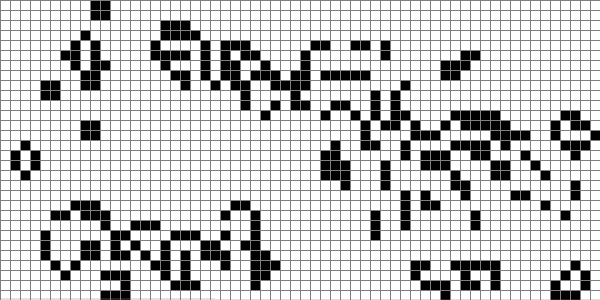
\includegraphics[width=8cm]{Pics/game_of_life.png}
\end{center}
\caption{The Game of Life}
\label{fig:game_of_life}
\end{figure}

\begin{figure}
\begin{center}
\includegraphics[width=8cm]{Pics/asteroids.png}
\end{center}
\caption{Asteroids shooter}
\label{fig:asteroids}
\end{figure}

\begin{figure}
\begin{center}
\includegraphics[width=8cm]{Pics/rpg.png}
\end{center}
\caption{RPG}
\label{fig:rpg}
\end{figure}

\begin{figure}
\begin{center}
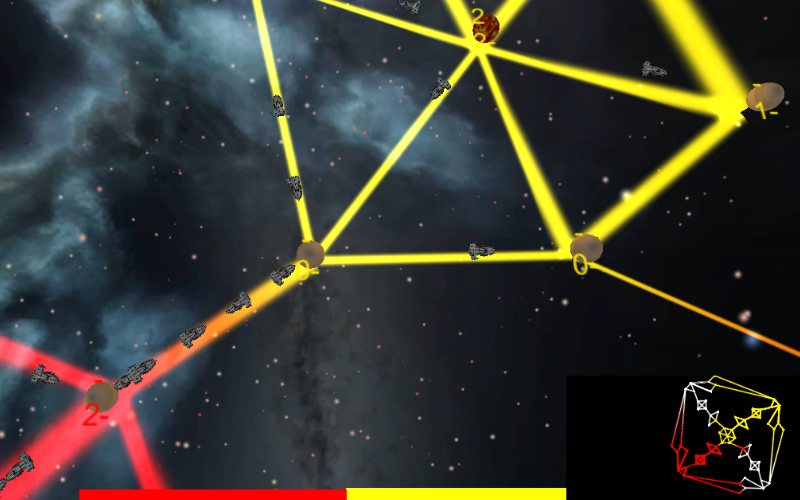
\includegraphics[width=8cm]{Pics/rts.png}
\end{center}
\caption{RTS}
\label{fig:rts}
\end{figure}

\begin{figure}
\begin{center}
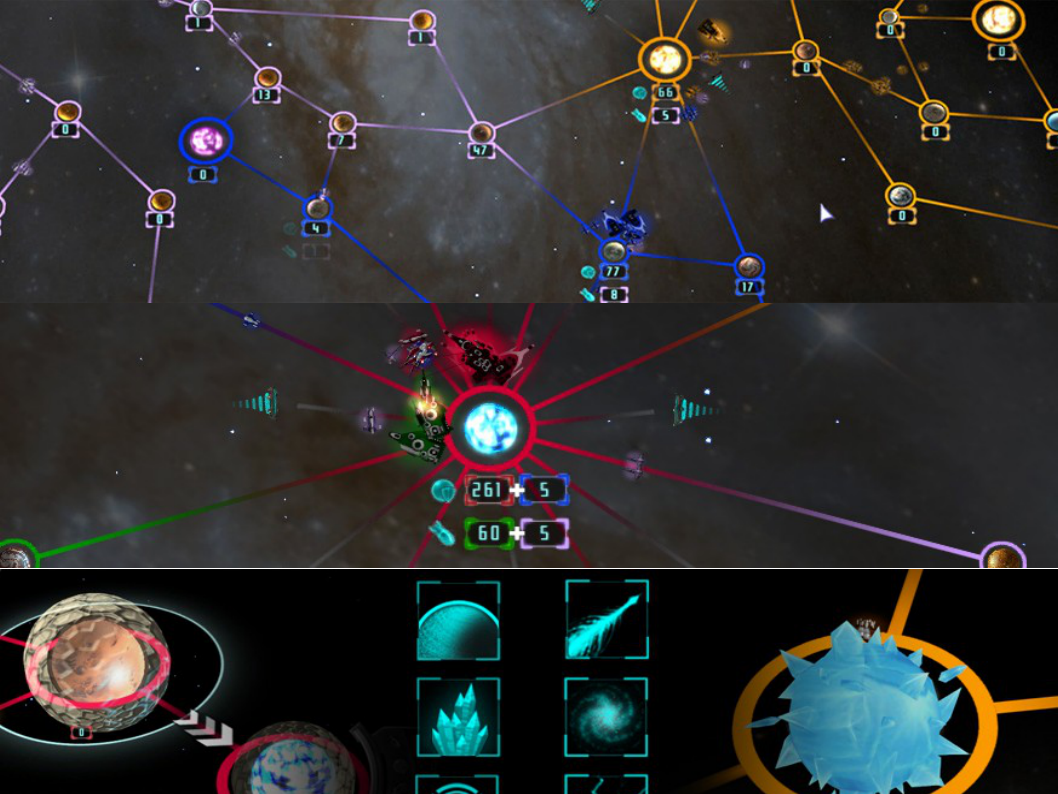
\includegraphics[width=8cm]{Pics/galaxy_wars.png}
\end{center}
\caption{Galaxy Wars}
\label{fig:galaxy_wars}
\end{figure}

The "game" is a zero-player game, meaning that its evolution is determined by its initial state, requiring no further input. One interacts with the Game of Life by creating an initial configuration and observing how it evolves.

The game is a zero-player game that takes an initial configuration of an orthogonal grid of square cells, and then evolves automatically. The player simply observes such evolution. Each cell is in one of two possible states: alive or dead. The state of a cell changes according to the state of its eight neighbors. At each iteration of the game, all cells transition in state according to the following simple rules: \textit{(i)} any live cell with fewer than two live neighbors dies; \textit{(ii)} any live cell with two or three live neighbors remains alive; \textit{(iii)} any live cell with more than three live neighbors dies; and \textit{(iv)} any dead cell with exactly three live neighbors becomes alive.

A Casanova game begins with the definition of a series of data structures, which are the world and its entities. The updates of an entity are contained in its rules, a series of methods that take the same name of the field they update at each tick; a rule is invoked automatically for each entity of the game, and it receives as input the current state of world, the current state of the entity being updated, and the time delta between the current frame and the previous frame. The result of computing a rule is stored in the game world only after all rules of all entities of the world have been computed successfully, that is, rules do not interfere with each other and can be computed in parallel. This avoids inconsistencies deriving from the state being only partially updated: the state is either at a time step or at the next, but no in-between representations are allowed. Entities may also have drawable fields such as text, sprites or 3D models; these fields are updated through rules as well, and at each tick all drawable entities are grouped into layers (layers specify blocks of drawable entities and the draw settings to use with them) which are then drawn. 

We start by defining the state of the game as a matrix of cells; the state also contains a boolean variable which will trigger the update of the cell matrix once per second. The world does not feature a sprite layer because for games that use only one sprite layer Casanova provides the developer with a predefined one that is called \texttt{default\_layer}:

\begin{lstlisting}
type World = { 
  Cells : List<List<Cell>> 
  UpdateNow : Var<bool> 
}
\end{lstlisting}

Each cell contains a value (which is 1 when the cell is alive and 0 when the cell is dead) and a list of its neighbors marked as \texttt{Ref}. The neighbors of a cell are just references to those cells, which are stored elsewhere in the game state. We inform Casanova of this fact by using \texttt{Ref}, thereby preventing Casanova from updating and drawing those cells every time they are reached from the game world. The value of the cell is updated every time an update is triggered (rather than at each tick), by summing the value of the neighbors and applying the rules mentioned above. The color of the cell sprite is updated to reflect its current value. 

\begin{lstlisting}
type Cell = { 
  NearCells : List<Ref<Cell>> 
  Value : int 
  Sprite : DrawableSprite }
  rule Value(world,self,dt) = 
    if state.UpdateNow then 
      let around = sum [for c in self.NearCells do yield c.Value] 
      match around with 
      | 3 -> 1 
      | 2 -> self.Value 
      | _ -> 0 
    else self.Value 
  rule Sprite.Color(world,self,dt) = 
    if self.Value = 0 then 
      Color.Black 
    else 
      Color.White
\end{lstlisting}

The initial state of the game creates the matrix of cells and initializes their neighbors. Each internal cell has exactly eight neighbors. The sprites layer and the cell sprite are also setup for each sprite. We omit only this listing as it is rather straightforward. The rules of the game are fired at every frame of the game that is roughly 60 times per second. Changing the entire matrix of cells this often would yield a chaotic result; for this reason we have defined the \texttt{UpdateNow} field in the game state, so that we can control when the rules are fired. The main script of the Game of Life simply waits for a second before toggling the \texttt{UpdateNow} value, and then it suspends itself until the next iteration of the update loop. When the script is resumed, it toggles \texttt{UpdateNow} again and finally it repeats. 

\begin{lstlisting}
let main world = 
  repeat co{ 
    do! wait 1.0<s> 
    world.UpdateNow := true 
    do! yield 
    world.UpdateNow := false } 
\end{lstlisting}

We could also add some basic interactivity by defining an input script which toggles updates when the user performs some input action.

\begin{lstlisting}
let input = [
    co{  
      do! wait_condition is_mouse_clicked
      do! wait_condition is_mouse_released
      return true } =>
     co{
       world.UpdateNow := true
       do! yield
       world.UpdateNow := false }
  ]
\end{lstlisting}

This way the game of life will tick at one step per second, no matter the framerate of the simulation, or when the user clicks the mouse. This is all there is to such a simple game.

\section{Making games with Casanova}
To assess the effectiveness of Casanova as a game development language we have undertaken two parallel development initiatives. The first initiative is \cite{CASANOVA_CODEPLEX}, where we have built a series of small samples that are easy to understand and manipulate; these samples are three different real-time games, chosen so as to see Casanova in action in different sub-domains of the real-time game genre, which we argue to be currently the most widespread. The second initiative is the game  \cite{GALAXY_WARS}, where we have used Casanova to build a much bigger game in order to test how well the language scales.

The small samples are an asteroid shooter game (Figure \ref{fig:asteroids}), an action/adventure game (Figure \ref{fig:rpg}), and a strategy game (Figure \ref{fig:rts}). We will not present the full samples themselves, which are available online. Instead, we will focus on a series of fundamental "development activities" that we believe to be nicely exemplified by our samples; these activities cover some of the most common and important pieces that can be customized, combined and extended into almost any game: \textit{(i)} defining a player avatar, handling his input and his shooting; \textit{(ii)} spawning obstacles randomly; \textit{(iii)} handling collisions between projectiles and obstacles; \textit{(iv)} representing the properties of a static map (cave) divided in rooms and cells; \textit{(v)} handling monsters and their AI (albeit a rudimentary one); \textit{(vi)} active entities such as bases or buildings that produce units; \textit{(vii)} selection-based input mechanisms. We show \textit{(i)}, \textit{(ii)}, and \textit{(iii)} from the asteroid shooter; \textit{(iv)} and \textit{(v)} are taken from the action/adventure game; finally, \textit{(vi)} and \textit{(vii)} are shown from the RTS game. 

By showing how to build these primitives in relative isolation from each other, we are effectively giving a library \footnote{Or rather a cookbook.} that allows to create games where a player avatar may interact with obstacles in arbitrary rooms, and where some objects are shot by the players, others simply store useful properties of the map, others move and have some AI, and others spawn units or manipulate the game world. From our experience, we note that many games can be built recombining such components. 

Since the games we present are simplified (it would be prohibitively difficult to build three large-scale games in this context) it is important to notice that these games represent just starting points that could be extended into full-blown games with more time and effort. An example of the extension process in action can be seen in \cite{GALAXY_WARS} (Figure \ref{fig:galaxy_wars}), an upcoming (commercial) strategy game that is derived from the RTS sample and that we built as an extended study of how to create non-trivial games with Casanova. Notice that the samples shown below simply are some of the most representative snippets, that is the omitted entities (for example asteroids and projectiles) are not significantly more complex than those shown in the following. 

Galaxy Wars is not the only project where Casanova has been used as a means rather than an end, even though it is the biggest. Casanova has also been used to build: \textit{(i)} two virtual city simulators that act as a testbed for AI techniques as part of a separate research effort; \textit{(ii)} an experimental AI for real-time planning; \textit{(iii)} a platform for building RTS games for both teaching and a Master Thesis; and \textit{(iv)} a serious game that teaches players cooperation in order to make a virtual organization survive. All of these examples can be accessed from the Casanova website \cite{CASANOVA_CODEPLEX}.


\section{Player avatar and shooting stuff}
The asteroid shooter game is a simple shooter game where asteroids fall from the top of the screen towards the bottom. The player aims the cannon and shoots the asteroids to prevent them from reaching the bottom of the screen. In this game we will describe how to define: \textit{(i)} the player avatar, his movement and shooting; \textit{(ii)} the spawning of obstacles such as asteroids; and \textit{(iii)} detection of collisions between asteroids and projectiles. The game world contains a list of projectiles, asteroids, the cannon, the current score, plus sprite layers for the main scene and the game UI \footnote{Compared to the Game of Life sample, here we need different sprite layers, and so we cannot rely on the default layer but instead we must declare our own.}. The game world removes asteroids and projectiles when they exit the screen or collide with each other, and it handles the current score (which is the number of destroyed asteroids). 

\begin{lstlisting}
type World = { 
  Sprites : SpriteLayer 
  UI : SpriteLayer

  StarsSprite : DrawableSprite 
  ScoreText : DrawableText

  Asteroids : Var<List<Asteroid>> 
  Projectiles : Var<List<Projectile>> 
  Cannon : Cannon 
  Score : int } 
  rule Asteroids(world,dt) = 
    [for a in state.Asteroids do 
       if a.Colliders.Length = 0 && a.Position.Y < 100.0<m> then
         yield a] 
  rule Projectiles(world,dt) = 
    [for p in state.Projectiles do 
       if p.Colliders.Length = 0 && p.Position.Y > 0.0<m> then
         yield p] 
  rule Score(world,dt) = 
    world.Score + 
      sum [for a in state.Asteroids do 
             if a.Colliders.Length > 0 then 
               yield 1]
  rule ScoreText.String(world,dt) = 
    "Current score = " + world.Score.ToString()
\end{lstlisting}  

% todo: split or expand
The player is represented by a cannon (similarly it might be represented by a moving ship) as an entity that contains a sprite, an angle, and a movement flag set from the input script that determines the variation of the angle and which is reset to 0 at every tick; the rotation of the sprite is taken from the current angle of the cannon:

\begin{lstlisting}
type Cannon = {  
  Sprite : DrawableSprite 
  Angle : float<rad> 
  Movement : Var<float> } 
  rule Angle(world,self,dt) = 
    self.Angle + self.Movement * dt
  rule Movement(world,self,dt) = 0.0
  rule Sprite.Rotation(world,self,dt) = self.Angle 
\end{lstlisting}

The input script that modifies the rotation of the cannon simply checks if the appropriate key is currently pressed, and if so the cannon movement value is set:

\begin{lstlisting}
co{ return is_key_down Keys.Left  } => co{ state.Cannon.Movement := 1.0 }; 
co{ return is_key_down Keys.Right } => co{ state.Cannon.Movement := -1.0 };
\end{lstlisting}


Similarly, projectiles are spawned whenever the space key is pressed; contrary to movement, though, after a projectile is spawned the script waits either the release of the space key or one-tenth of a second to ensure that projectiles are not shot with a frequency of one per frame as long as the user keeps pressing the space bar. 

% todo: split or expand
It is worth noticing that such a simple activity would require a timer-based event infrastructure that can be quite tedious to write in a traditional language; for example, a timer to wait after the spawning of a projectile would need to be stored, declared, and consulted manually at each tick. Instead of writing that, in Casanova we just write the following code that automatically handles the creation and management of invisible timer variables:

\begin{lstlisting}
co{ 
   do! wait_condition (is_key_down Keys.Space) 
   do! wait_condition (is_key_up Keys.Space)
         || wait 0.1<s>
   return true } =>
co{  
  state.Projectiles.Add 
    { Sprite = { Path = "projectile.jpg"; Layer = world.Sprites } 
      Position = Vector2(50.0<m>, 0.0<m>) 
      Velocity = Vector2(cos(state.CannonAngle),sin(state.CannonAngle))
      Colliders = [] } } 
\end{lstlisting}

Asteroids are generated with a simple recursive script that waits a random amount of time and then adds the asteroid to the game world before looping:

\begin{lstlisting}
  repeat co{ 
    wait (random(1.0<s>,3.0<s>)) 
    state.Asteroids.Add 
      { Sprite = { Path = "asteroid.jpg" Layer = world.Sprites }
        Position = vector2(random(0.0<m>,100.0<m>),0.0<m>) 
        Velocity = vector2(0.0<m/s>,random(5.0<m/s>,20.0<m/s>))
        Colliders = [] } } 
\end{lstlisting}

Collision detection is simple as well: both asteroids and projectiles compute the list of colliders against themselves; this list is then used in the query shown above in the definition of the game world to cull away asteroids that are hit by projectiles:

\begin{lstlisting}
type Asteroid = { 
  ...
  Colliders : List<Ref<Projectile>> } 
  ...
  rule Colliders(world,self,dt) = 
    [for x in world.Projectiles do
       if distance(self, x) < 10.0f then
         yield ref x] 
\end{lstlisting}

\section{Game map and monsters with AI}
The action/adventure game features a player-controlled character that moves between various rooms fighting monsters and drinking health-increasing potions. In the game we see how to handle: \textit{(iv)} a game world comprised of rooms and cells, where each room is divided into cells; and \textit{(v)} monsters who fight against the player with some AI. 

% todo: expand
The game state contains, among other entities (such as the player) and sprite layers (to draw the game entities and the UI) the current room the player is in. A room is defined as a series of cells and a list of monsters; monsters are removed from a room whenever they are killed when fighting against the player:

\begin{lstlisting}
type Room = { 
  Cells    : List<List<Cell>> 
  Monsters : list<Monster> } 
  rule Monsters(world,self,dt) = 
    [for m in self.Monsters do 
       if m.Health > 0 then
         yield m]
\end{lstlisting}

% todo: expand; we could instead have defined another type of cell, the portal cell, which contains ...
Each cell contains, most notably, a nullable reference to the room it leads to in case it is a portal, a list of neighboring cells, a boolean value that determines if the player is in the cell, plus a sprite for drawing it:

\begin{lstlisting}
type Cell = { 
  Position   : Vector2<m> 
  Sprite     : DrawableSprite 
  HasPlayer  : bool
  Door       : Option<Ref<Room>> 
  Neighbours : list<ref<Cell>> } 
  rule HasPlayer(world,self,dt) = 
    world.Player.Position = self 
\end{lstlisting}

% todo: expand; movement, fighting, appearance
Monsters are one the most important entities of the game. A monster contains fields to describe its position (the cell it’s currently in), its target (the cell it’s traveling to), the delta of its position between the current cell and the target cell, its sprite (for drawing it) and its current health. The monster rules update all of its fields; its health is updated when the player is in the same cell, the current cell is changed when the target cell is reached (and the target cell is set to null to stop the movement), and so on:

\begin{lstlisting}
type Monster = { 
  Position      : Var<Ref<Cell>> 
  Sprite        : DrawableSprite
  Health        : int
  Damage        : Var<int> 
  MoveTarget    : Var<Ref<Option<Cell>> 
  PositionDelta : Vector2 } 
  member Movement(world,self,dt,on_arrived,on_moving) = 
    match self.MoveTarget with 
    | Some target 
        when distance(self.Position + self.PositionDelta, 
                      target.Position) < 0.1 -> 
      on_arrived target 
    |Some target -> on_moving() 
    | None -> on_moving() 
  rule Health(world,self,dt) = 
    if self.Position.HasPlayer && world.UpdateNow then 
      self.Health - world.Player.Damage * random(1,4) 
    else self.Health 
  rule Position(world,self,dt) = 
    Movement(world,self,dt,id,
             fun () -> self.Position) 
  rule MoveTarget(world,self,dt) = 
    Movement(world,self,dt,fun () -> None,
             fun () -> self.MoveTarget)   
  rule PositionDelta(world,self,dt) = 
    Movement(world,self,dt, 
      fun () -> self.PositionDelta + 
                  dt * normalize(target.Position - 
                                 self.Position.Position), 
      fun () -> self.PositionDelta) 
  rule Sprite.Position(world,self,dt) = 
    self.Position + self.PositionDelta
\end{lstlisting}

% todo: expand, re-order
Two things in particular should be noted in the listing above. We used higher-order-functions \footnote{Higher-order-functions are those which take as some of their input parameters other functions.} to abstract away the boilerplate pattern of evaluating something when the monster is moving, and something else when the monster is still; we do so in the \texttt{Movement} method, which takes as input the \texttt{on\_arrived} and \texttt{on\_moving} functions and then invokes them as appropriate. We use the \texttt{Movement} method in the \texttt{Position}, \texttt{MoveTarget}, and \texttt{PositionDelta} rules, instead of repeating the almost identical code every time. Also, we make use of a global boolean variable, \texttt{world.UpdateNow}, which is ticked by a script and which is used as a guard to compute rules such as those for the monsters battles; this boolean is similar to the \texttt{UpdateNow} boolean that we have seen in the Game of Life. 

Monsters also have a rudimentary AI which chooses a destination cell for the monster to travel to, and which keeps doing so until the player is in the current room. This allows monsters to not weigh computationally when the player cannot interact with them, since he is in a different room. 

% todo: expand "let target_cell = ..."
\begin{lstlisting}
let monster_AI (monster : Monster) = 
  repeat co{ 
    if monster.Health > 0 then  
     if world.UpdateNow && random(0, 20) < 1 && 
        monster.MoveTarget = None then 
       let target_cell = ...
       do monster.MoveTarget := Some target_cell) } 
     || co{ wait_condition (fun () -> 
              world.CurrentRoom <> monster.Position.Room)
\end{lstlisting}

% todo: expand
Notice the use of the \texttt{(||)} operator which runs two scripts concurrently, that is until either of the scripts has completed; its use in this scenario allows us to stop the repeating script as soon as the current room changes: this disables the script for the monsters in the previous room, thereby avoiding to accumulate wasteful running scripts for rooms visited previously.

\section{Active map entities and selection-based input} 
The strategy game features a series of planets that produce ships, which can then be sent to conquer other planets. In this game we see: \textit{(vi)} active entities, such as planets, that represent complex components of the game scenario; and \textit{(vii)} complex selection-based input mechanisms based on the selection of game entities and the interaction with the selected entities.

% todo: expand
We represent the game world as a series of planets, ships, plus the currently selected planet; the game world also contains sprite layers for rendering the game entities and UI, plus a boolean that (in the same spirit of the \texttt{UpdateNow} field in the Game of Life) allows the game battles to tick at fixed time intervals rather than at each tick of the game:

\begin{lstlisting}
type World = { 
  Sprites      : SpriteLayer 
  UI           : SpriteLayer 
  Planets      : List<Planet> 
  Fleets       : Var<List<Fleet>> 
  TickBattles  : Var<bool> 
  SourcePlanet : Var<Option<Ref<Planet>>> } 
  rule Fleets(world,dt) = 
    [for f in self.Fleets do
       if f.Alive && (not(f.Arrived) || f.Fighting) then
         yield f]
\end{lstlisting}

Planets manage the battles in their orbit (to determine the owner of the planet) and ship production; in addition to their other fields, planets store the current owner, the number of allied ships stationed on the planet, and the percentage of production for the next ship; furthermore, a planet maintains a list of the fleets that are attacking or defending it:

\begin{lstlisting}
type Planet = { 
  Owner             : Player
  Armies            : Var<int<Ship>>
  FractionalArmies  : float<Ship>
  AttackingFleets   : List<Ref<Fleet>>
  ReinforcingFleets : List<Ref<Fleet>>
  ... } 
  rule Owner(world,self,dt) = 
    if self.Armies <= 0 && self.AttackingFleets.Length > 0 then
      self.AttackingFleets[0].Owner 
    else 
      self.Owner 
  rule Armies(world,self,dt) = 
    if self.Armies <= 0 then 
      sum [for a in self.AttackingFleets do
             if a.Owner = self.AtackingFleets[0].Owner then
               yield a.Armies] 
    else 
      let damages = sum[for f in self.AttackingFleets do 
                          yield random(1,3)] * state.TickBattles 
      let reinforcements = sum[for f in self.ReinforcingFleets do
                                 yield f.Armies] 
      self.Armies + int(self.FractionalArmies) - damages + reinforcements 
  rule FractionalArmies(world,self,dt) = 
    self.FractionalArmies + (dt * self.Production) - floor(self.FractionalArmies) 
  rule AttackingFleets(world,self,dt) = 
    [for f in state.Fleets do
       if f.Target = self && f.Owner <> self.Owner && f.Arrived then
         yield f] 
  rule ReinforcingFleets(world,self,dt) = 
    [for f in state.Fleets do
       if f.Target = self && f.Owner = self.Owner && f.Arrived then
         yield f]
\end{lstlisting}

% todo: expand
Input scripts manage the selection of a new planet by waiting for a left click of the mouse and then setting the \texttt{SourcePlanet} field of the game world:

\begin{lstlisting}
co{ do! wait_condition mouse_clicked_left
    do! wait_condition mouse_released_left
    let clicked = 
      [for p in world.Planets do 
         if distance(p.Position,mouse) < 10.0 && 
            p.Owner = Human then 
           yield p] 
    if clicked <> [] then
      return Some(clicked.[0])
    else 
      return None } =>
  fun p -> co{ return world.SourcePlanet := Some(p) }
\end{lstlisting}

% todo: expand
Similarly, when the user right clicks then if there is an active selection some ships are sent:

\begin{lstlisting}
co{ do! wait_condition (mouse_clicked_right && 
                        world.SourcePlanet <> None)
    do! wait_condition mouse_released_left
    let mouse = mouse_position() 
    let clicked = 
      [for p in world.Planets do
         if distance(p.Position,mouse) < 10.0 then
           yield p] 
    match clicked with
    | clicked::_ ->
      return Some(clicked.[0],world.SourcePlanet.Value) 
    | [] ->
      return None } => 
  fun (source,target) -> co{ return mk_fleet source target } 
\end{lstlisting}


\section{Recombining the samples}
The samples just shown are simple but significant snippets extracted from existing games. They represent fundamental activities in game development, since virtually all games feature at least some of these aspects; we have shown how to implement a user-controlled player that moves and shoots, we have shown how to create active obstacles with some intelligence that make the game interesting to play, and we have shown how to define static objects that are part of the scenario and that interact with the player. The samples above have indeed been recombined in the Galaxy Wars \cite{GALAXY_WARS} game, an Open Source commercial game developed in parallel with Casanova and used as a testbed for Casanova techniques. Galaxy Wars has been built as an extended study of how to create non-trivial games with Casanova. More projects, which mostly feature research simulations, have used Casanova as their framework: from virtual cities for AI research to teaching tools and even to serious games, Casanova is being put to the test extensively.

\section{Hand written optimizations}
The presented samples show no algorithmic optimizations in place, relying entirely on the runtime to provide sufficient performance. A note must be added on the fact that Casanova easily supports any algorithmic optimizations that a game developer may need to add. The least sophisticated way to add such an optimization would very simply be to use a variable to store some optimized data structure in the game world, and then using a script to update this structure in a loop. The resulting code would have the following structure:

\begin{lstlisting}
type World = {
  ...
  OptimizedStorage : Var<OptimizedStorage>
}

...

repeat
  co{ 
    do world.OptimizedStorage := update_optimized_storage world
    do! yield  
  }
\end{lstlisting}

This techniques simply replicates a traditional game loop inside Casanova itself, in order to maintain an updated data structure that stores optimized lookup tables or other similar helps to the computation. An advantage that Casanova offers at no additional cost is that if the update of the optimized data structures of the game world is expensive, then its computation may be easily split across multiple ticks, further improving the game performance:

\begin{lstlisting}
repeat
  co{
    let step1 = update_optimized_storage1 world
    do! yield
    let step2 = update_optimized_storage1 world step2
    do! yield
    ...
    do world.OptimizedStorage := update_optimized_storageN world stepN
    do! yield  
  }
\end{lstlisting}

Of course, rules may also be used to implement such a system without scripts and mutability. A significant difference between using rules rather than scripts is that for the results of rules to propagate to other rules then it takes multiple ticks, and so rules force the developer to implement the second snippet of the two shown above. If the optimized data structure must be computed entirely in one frame, and must be updated at every frame, then scripts are the most effective solution.
 

\chapter{Evaluation of Casanova}
\footnotetext{This chapter is partially derived from the papers \cite{CASANOVA_ICEC, CASANOVA_ACG, CASANOVA_SCRIPTS, CASANOVA_EICS}.}
\label{chap:evaluation}
We now present an RTS game we used as a case study, created with Casanova, and the benchmarks that test the action implementation. In the game players must conquer a star system made up of various planets. Each planet builds fleets which are used to fight the fleets of the other players and to conquer more planets. A planet is conquered when a fleet of a player is near it and no other enemy fleet is defending it.

\subsection{Case study}

Three actions are required in this game: The first action, called \texttt{Fight Action}, defines how a fleet fights enemy fleets in range. The fight action subtracts $0.5 \cdot dt$ \texttt{life} points from the in-range enemy fleet during every frame (action tick).

\begin{lstlisting}[language=Caml]
Fleet = {Position: Rule Vector2;FightAction: FightAction;Owner: Ref Player;Life: Var float32;Fight: FightAction }
\end{lstlisting}

The Fight Action is defined as follows:

\begin{lstlisting}[language=sql]
FightAction = TARGET Fleet; RESTRICTION Owner <> Owner; RADIUS 150.0; TRANSFER CONSTANT Life - 0.5;
\end{lstlisting}

The target is an entity of which the type is \textbf{Fleet}. The condition to execute the action is that the fleet must be an enemy (i.e., not the player). The \texttt{attack range} is 150 units of distance. 0.5 \texttt{life} points are subtracted for every attack.

The second action is called \texttt{BuildAction}. It allows a planet to create a ship. In order to build a ship, a planet must gather 10 mineral units. Each planet has a field called \texttt{GatherSpeed} which determines how fast it gathers minerals. Every tick the planet's mineral stash is increased by this amount. This action is a threshold action where the threshold value is the minerals of the planet. As soon as the threshold value is reached, we set the field \texttt{NewFleet} to TRUE (it is used by the engine to create a new fleet), and \texttt{Minerals} to 0 to reset the counter. The planet and its actions are:

\begin{lstlisting}[language=Caml]
Planet = {Position: Vector2;Owner: Rule Ref Player;NewFleet: Rule bool;BuildAction:BuildAction;EnemyOrbitingFleetsAction : EnemyOrbitingFleetsAction;GatherSpeed: float32;Minerals: Var float32 }
\end{lstlisting}

\begin{lstlisting}[language=sql]
BuildAction =
TARGET Self; TRANSFER CONSTANT Minerals + GatherSpeed; THRESHOLD Minerals 10.0; OUTPUT NewFleet := true; OUTPUT Minerals := 0.0
\end{lstlisting}

A Casanova rule is appointed to read the value of NewFleet and, when it is true, to spawn a new fleet.

The third action is required to check if a planet can be conquered by a fleet. A fleet can conquer a planet if there is no enemy fleet near it and if it is sufficiently close. Thus the action definition is the following:

\begin{lstlisting}[language=sql]
EnemyOrbitingFleetsAction =
TARGET Fleet; RESTRICTION Owner Not Eq Owner; RADIUS 25.0; INSERT Owner -> EnemyOrbitingFleets
\end{lstlisting}

The action will add an enemy fleet close enough to change the owner of the planet.

%Even the concept of drawing lasers can be implemented using the INSERT clause simply adding it to \texttt{FightAction} which inserts in a list all the targeted ships positions. In this way we can draw a laser from the source position to the target position. We omit this aspect for brevity.

\subsection{Evaluation}

We evaluated the performance of our approach with the case study, and two extra examples: an asteroid shooter, and an expanded version of the case study with more complex rules. All were implemented in Casanova. Table \ref{tab:code_length} shows a code length comparison between the REA implementation and standard Casanova rules for all three.

We note that in games with basic dynamics the code saving is low, due to the fact that there are few repeated patterns. The advantage of using REA becomes evident in a game with actions involving many types of targets, such as the expanded case study. Furthermore, we managed to drastically increase the performance of the game logic: as Figure \ref{fps_chart} shows, using REA (labeled ``with actions'') results in a speedup factor of 6 to 25, due to automated optimizations in the query evaluation. We also note that our implementation is flexible and general since it is possible to use actions to express a behaviour, such as a projectile collision, which is outside the domain of RTS games and traditional resource-based systems.

\begin{table}
\centering
\caption{CS (case study), Asteroid Shooter and Expanded CS code length}
\label{tab:code_length}
\begin{tabular}
{|l|c|c|c|c|c|c|}
\hline
& Game Entities & Rules & Actions & Total\\
\hline
\textit{CS with REA} & 41 & 71 & 19 & 131\\
\hline
\textit{CS without REA} & 40 & 90 & 0 & 130\\
\hline
\textit{Asteroid shooter with REA} & 33 & 33 & 6 & 72\\
\hline
\textit{Asteroid Shooter without REA} & 34 & 44 & 0 & 78\\
\hline
\textit{Extended CS with REA} & 135 & 138 & 40 & 313\\
\hline
\textit{Extended CS without REA} & 135 & 328 & 0 & 463\\
\hline
\end{tabular}
\end{table}
\begin{figure}
\centering
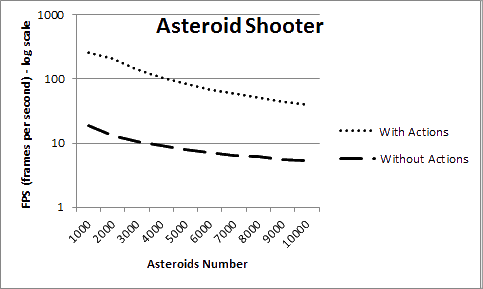
\includegraphics[scale=0.7]{Shooter.png}
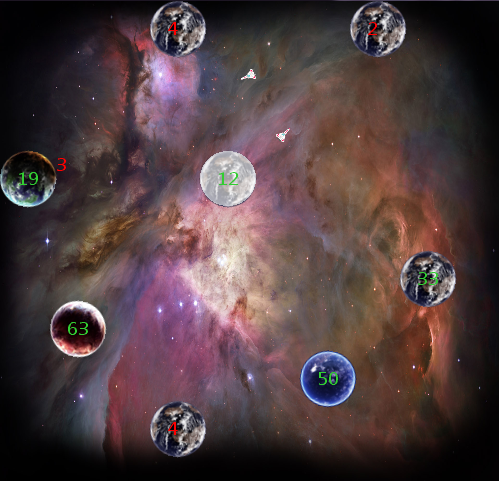
\includegraphics[scale=0.7]{RTS.png}
\caption{Frame rate as a function of numbers of entities.}
\label{fps_chart}
\end{figure}  

\chapter{Discussion}
\label{chap:discussion}
In this section we sum up the content of this work, with particular focus on: \textit{(i)} how Casanova answers the original questions of this thesis; \textit{(ii)} what are the limitations of Casanova that may be solved with small extensions; \textit{(iii)} what are the limitations of Casanova that may be solved with a major design effort or not at all.

\section{Original research questions}
The research questions studied by this work are listed in Chapter \ref{chap:introduction}, but we sum them up here again:

\begin{tabular}{ | l | p{6cm} | }
\hline
\textbf{requirements} & what are the general requirements common across development of most games? \\
\hline
\textbf{exploration} & what are the most representative game development systems and languages? \\
\hline
\textbf{design} & what is a general and simple to use programming language that fulfills the game development requirements? \\
\hline
\textbf{evaluation} & Does such a language work for making games in practice? How does such it compare to other game development systems? \\
\hline
\end{tabular}


We have identified a set of requirements by observing which are the most common tasks performed by game developers while making a game. These are tasks that allow the simulation of a virtual world that is updated in real-time, steered by the user input, while providing a real-time visual representation of the virtual world. We have identified these requirements through our experience with game development, by studying the architectures of multiple game development tools and libraries, and by a survey of the fundamental literature of game development which all mentions these constructs. Even though we believe to have identified a set of universal, core requirements of games, we are also certain that further important requirements exist that we are not considering. We also believe that the requirements we consider here are the first that should be tackled, since considering more exotic issues would require that these are solved first.

A preliminary study of the available game development systems yielded dozens of powerful systems, engines, and frameworks, plus various languages. As game development is a complex activity, so game development tools are large and difficult to learn. To narrow our focus we started by restricting ourselves to only those tools that are aimed at making the same kind of games that Casanova supports, namely serious, research, and indie games. Secondly, we picked the three systems that seem the most popular in terms of available books, tutorials, documentation, and sample projects.
Choosing game development languages on the other hand was simpler, since there are not many available. We picked three languages that exemplified that language design does not need to be a derivative effort that yields yet another imperative language with objects; we picked languages that show provocative new semantic and syntactic structures.

We designed Casanova around the identified requirements for games, by choosing the design philosophy of less-is-more. We tried to find the smallest set of orthogonal syntactic primitives that would allow the expression of the desired semantics. We built Casanova semantics in order to express game concepts of input, drawing, time flow, state machines, and few other primitives. We used our type system to support useful correctness enforcers such as dimensional analysis. We built an implementation that optimizes run-time by taking advantage of the semantics of the game, for example by adding multi-threading automatically where it is safe to do so.

We evaluated Casanova by showing how actual game snippets can be produced in it, and by identifying exemplar game development tasks such as defining an avatar, interacting and moving in a virtual environment with entities representing objects and monsters, and so on. We then proceeded to a comparison of Casanova with existing game development systems in order to assess complexity. We also offered some benchmarks that quantified certain indicators of performance and verbosity. These benchmarks compare coroutine systems across multiple scripting languages commonly used in games, in order to assess how well Casanova stacks against them in one of its most complex (and computationally intensive) sub-systems. Finally, we performed some user studies with students ranging from complete beginners in Computer Science, to advanced programmers learning the finer points of game development.

\section{Extension opportunities for Casanova}
We now discuss some of the aspects of Casanova that could be improved upon. We explain how rendering could be made more powerful, how we are building a standard library of components ready for reuse, how we are creating an IDE for supporting the Casanova language directly, and how we are extending the language in order to support general-purpose networking and AI facilities. We conclude with a note on the applicability of Casanova to AAA games.

\subsection{Rendering}
Rendering in Casanova is the weakest aspect of the current implementation and design. On one hand we believe that rendering is almost not an open problem anymore, and that much of the current research on rendering is actually focused on technical, engineering, and approximation efforts \cite{GPU_GEMS_1, GPU_GEMS_2, GPU_GEMS_3} rather than on fundamental understanding of photo-realistic lighting models \cite{CHAPTER_9_RENDERING_EQUATION}. Since we aim at solving fundamental issues with game development in general, we have chosen to create a first rendering system that allows testing of the rest of Casanova, with the objective to integrate some other rendering engine, possibly even Unity itself (or any other engine that supports .Net/Mono bindings), when the framework is sufficiently mature that the current drawing facilities become inadequate.

\subsection{Standard library}
Casanova also lacks a standard library. A standard library for a system such as Casanova would provide sets of entities that cooperate with each other in order to provide some pervasive game functionality like physics, or even whole game skeletons for different genres. Such a library would allow us to inject past experience in making certain games into Casanova, thereby further reducing the difficulty of game development with the framework; unfortunately, building such a library requires a substantial engineering effort, and is partially beyond the current scope of this work. Still, we are slowly increasing the size of the Casanova library of utilities by generalizing the various portions of the games we build when we see components that may be of broader utility.

\subsection{IDE}
The current IDE for Casanova is also a major source of future work. On one hand the implementation is lacking all the code-completion technologies that many programmers are used to, and which make coding much simpler as it allows to keep track of the source code structure automatically. Code completion also helps greatly when getting confidence with new and unknown libraries, since it makes it possible to interactively explore them without reading lots of documentation before hand. 
The lack of a proper compiler currently requires developers to write Casanova embedded in F\#. While this does not have many significant shortcomings, the language used this way loses in simplicity and power. One important disadvantage of the lack of a compiler though is that query optimizations are not active at the moment, because they require syntactic transformations that are hard to encode from F\#. Also, some small syntactic improvements (especially, but not limited to, the declaration and lookup of rules) would improve code readability. 

Further extensions that a proper language could support include a better code generator for state machines from coroutines. The current implementation instances multiple anonymous functions, namely one for each binding operation. This means that coroutines allocate memory that is often used for a very short time. Garbage collection of Casanova programs could then benefit from an optimization that uses, for example, pooling of the coroutine continuations to reduce generated garbage. Such a modification would yield a very small improvement on those implementations of the runtime that employ a modern, generational garbage collector \cite{CHAPTER_9_GENERATIONAL_GC}. The gains could be much bigger on platforms such as the XBox or tablet PCs where garbage collection uses a slower implementation \cite{CHAPTER_9_XBOX_GC_ISSUES}.

\subsection{Networking}
Networking is a major extension that is currently under construction for Casanova. A prototype implementation is  sketched in Appendix \ref{chap:networking}. Our goal is to build a system that is general, robust, and efficient. We are building such a system which, at its core, is a distributed synchronization mechanism that implements an eventually consistent serialization and deserialization of the game world from the host to the client. The eventual consistency arises from the fact that transferring the game world from the host is done many times per minute, and so information lost during one transfer will simply be expected in a future transfer. Also, the client will have to send the input events to the host in order for it to propagate the input responses to the remaining clients.

One major concern of our networking system is also performance and responsiveness. For this reason, we are building incremental transfers, data compression, and even local prediction techniques on the client side in order to minimize bandwidth and perceived delays.

\subsection{AI}
We are studying how to build a general system for AI, as described in Appendix \ref{chap:goap}. We believe that planning may be a good candidate technique for games in general, given that the simplest and most common technique for AI in games (finite state machines) is already supported with coroutines, and planning is the foundation for many reasoning systems, from path-finding to more complex decision-making. In particular, we are integrating a technique known as Goal-Oriented Action Planning \cite{APPENDIX_C_GOAP_BOOK} which allows agents to quickly find, thanks to heuristic search, action plans in order to satisfy all the preconditions that are required in order to satisfy a goal. The technique is already giving promising results in our systems, it easily incorporates path-finding, and it yields agents that seem deliberate and logical in their actions, which all contribute to reaching the final goal.

\subsection{AAA games}
An important issue with Casanova is that, for obvious constraints of time and resources, we have never developed a AAA game with it. It is understandable that AAA developers may have many reasons for not using Casanova. After all, a AAA studio has a team of programmers trained in traditional tools and languages, large libraries of existing code that should be leveraged as much as possible, and even a certain aversion to risking a big investment by using something that is not time-tested. This said, it is important to realize that Casanova helps development of games regardless of their scale. Whether they are tiny games built in a few hours, larger indie-games built in a few months, or huge AAA games that take years to develop, the same advantages of correctness, convenience, and expressive power would stand. For this reason we conclude that large development studios should at least consider the lesson of Casanova in order to take advantage of its most useful aspects within (or at least close to) the boundaries of their active development practices.


\section{Shortcomings of Casanova}
Casanova also has some shortcomings which determine what games it cannot be used to build. The main shortcomings that we have identified are: \textit{(i)} the inability to do low-level optimizations; \textit{(ii)} the required mindset shift for imperative programmers; \textit{(iii)} the rarely-seen ML syntax; and \textit{(iv)} the difficulty of expressing complex rendering tasks such as shaders.

\subsection{Low-level optimizations}
Most games, especially (but not limited to) larger titles, are sometimes faced with a need for optimization at a very low level, for example in order to run on less powerful hardware such as tablets or smartphones, or to support complex scenarios that require making use of all the available computational power.

Low-level optimizations may include control over memory allocations and deallocations, doubly-linked lists to quickly move an object from one group to another, and even re-writing some central portions of the inner loop in assembly. Unfortunately, these optimizations come at a cost: very little can be said (or controlled) about such portions of code, which would possibly break all the other semantic structures of the language. We argue that supporting low-level optimizations should be done only if we can at the same time retain all the properties of the system. Alternatively, we believe that better automated optimizations could further remove the need or desire to perform such optimizations. In the end though, Casanova is explicitly not aimed at AAA games, which are the only ones employing such aggressive optimizations techniques; for this reason Casanova emphasizes high-level abstraction at the expense of low-level optimization.

\subsection{Imperative mindset shift}
Casanova is a hybrid language that uses declarative/functional primitives for a large part of the game (namely, rules). The fact that rules may not affect any entity excluded the one they are operating on may cause some difficulties in programmers used to imperative operations that allow them to potentially modify any entity in the program from virtually any place in the code. This form of programming though may encounter difficulties in scaling with larger projects, since complex side-effects may get out of hand and break invariants that are otherwise assumed. Learning a declarative/functional way of thinking about programs can be a valuable skill in that it allows to cleanly split functionality in such a way that testing may be easier, and also that reasoning on the program may be easier as well. This said, programmers coming from an imperative background may require a larger initial effort than people with no background in programming at all, as we have discussed in Chapter \ref{chap:evaluation}.

\subsection{Unusual syntax}
Similarly to the issues with the declarative/functional style of programming, the syntax of Casanova is based on the lesser known syntax of ML and F\#. This syntax is widely used nowadays, but not as much as that of other imperative languages such as C, Java, C\#, or Python.
Building an alternate syntactic front-end would not change the underlying semantics or possibly even the backend implementation of our system, but it would still require substantial work in both design and implementation. Using a more common syntax, though, may reduce the perceived steepness of the learning curve of Casanova and thus remains a desirable feature.

\subsection{Advanced rendering}
Programming complex rendering operations is, as of now, delegated to the underlying rendering mechanisms of the graphics engine used by Casanova. We argue that it would be desirable to be able to express complex rendering operations in Casanova itself, for example by defining shaders, render target, etc. with separate syntactic abstractions. Unfortunately this would require a major design and implementation effort, and as such it must be relegated to our future intentions.

\subsection{Other languages}
As our implementation language, we picked F\#. The choice of F\# was motivated by its balance of performance, game development libraries, IDE support, and meta-programming through monads and reflection. Even though our experience in using our own libraries confirms F\# to be a good choice, there are multiple aspects that could not be translated from the Casanova language. 

Powerful languages such as C++ and Haskell are a good fit for a game development system such as Casanova. Interestingly, neither of them is capable of expressing Casanova constructs easily, and both require significant effort. Haskell would need an extension to the language (namely Generic Haskell \cite{APPENDIX_E_GENERIC_HASKELL}), while the degree of meta-programming used in C++ creates problems with the type inference of template parameters and often results in incomprehensible error messages. 

Haskell type-classes, in particular, allow us to code advanced meta-programming constructs, while still retaining some degree of assistance from the compiler in terms of meaningful error messages, partial compilation (to speed up compile-times for large programs), and other similar advantages. Of course, modern pragmatic languages such as C\#, F\#, Java, and the like allow the exploration of types at run-time with dynamic, unsafe operations known as \textit{reflection}. This allows these languages to retain high levels of expressivity for complex patterns (such as dependency injection), but with the penalty of lower run-times and no validation from the compiler (programs that use reflection may encounter unforeseen and catastrophic failures if used naïvely). Thanks to reflection and monads, Casanova is currently implemented as an embedding into F\#.

We make one final remark about the choice of F\# instead of a dynamic language that would not have required the "contorsions" of reflection to implement rules. For example, in Python, invoking rules would have been much simpler and would not have used reflection; moreover, Python (partially) supports coroutines and suspension mechanisms with its feature of generators.

\textit{These difficulties in adapting existing languages to Casanova suggests that Casanova is indeed a novel solution that offers significant features that are orthogonal to those present in existing languages.}

We leave as a challenge the successful implementation of Casanova inside other existing languages.
 

\chapter{Conclusions}
\label{chap:conclusions}
%% Changed by PS, April 4, 2014.

\section{Future work}
\label{sec:future_work}
The Casanova 2 language is capable of implementing usable and quite complex games. The language, while usable, is currently still in development as it misses a few features. In particular, support for multiplayer games is at this moment lacking. We believe that the existing mechanisms for handling time offered by Casanova 2 could be augmented with relatively little effort in order to greatly simplify the hard task of building multiplayer games. This is part of future work, that we are currently engaging in. We are also doing usability studies using students from various disciplines and backgrounds.

The high level view of the game that the Casanova 2 compiler provides can be exploited in order to improve the programmer experience. This means that we could use tools for code analysis (such as abstract interpretation \cite{nielson1999principles} or type system extensions) in order to better understand the game being built, and to help with correctness analysis, performance analysis, or even optimization.


%\subsection{User study}
%We wish to perform an in-depth user study for Casanova 2 to improve usability in the development process. We have already performed a partial (and quite promising) small user study which we will extend and complete.


%We have performed the following test: we gathered a group of students of game programming and a group of students of game design. We gave them a series of Casanova 2 samples, printed on paper. Each student had to guess the functionality of each sample, and sketch a screen-shot. Furthermore, each student also provided some additional feedback on the language.

%The samples were: (\textit{i}) a string of text moved around the screen with the keyboard, (\textit{ii}) a string of text that moves along a predefined path automatically, and (\textit{iii}) an asteroid shooter.

%Eleven (over a total of thirteen) students understood the samples completely, both drawing the screen-shots and explaining the dynamics of the game correctly. Two students were lost on the syntactic differences between Casanova 2 and the more familiar C-like syntax. The direct feedback was mostly centred around a series of common observations, which are reported in Table \ref{students_feedback}. For each observation, the table reports how many times we encountered it.

%\begin{table}[!t]
%% increase table row spacing, adjust to taste
%\renewcommand{\arraystretch}{1.3}
% if using array.sty, it might be a good idea to tweak the value of
% \extrarowheight as needed to properly center the text within the cells

%\caption{Feedback from students}
%\label{students_feedback}
%\centering

%% Some packages, such as MDW tools, offer better commands for making tables
%% than the plain LaTeX2e tabular which is used here.
%\begin{tabular}{|c||c|}
%\hline
%Syntax is unfamiliar at first & 3\\
%\hline
%Syntax is clear & 8\\
%\hline
%Indentation instead of parentheses is a downside & 2\\
%\hline
%List processing with queries is very effective & 1\\
%\hline
%Rules are a good abstraction for games & 2\\
%\hline
%\end{tabular}
%\end{table}

%We also built a significantly bigger sample, which we asked only three students to study. The sample is a checkpoint-based RTS (see Figure \ref{RTS game} for a screenshot). All students correctly identified the game mechanics, and provided some additional feedback. Most of this feedback overlaps with that obtained for the samples, but some new observations emerge. Arguably, some patterns become visible only with larger samples:
%\begin{itemize}
%\item \texttt{wait} and \texttt{when} are very powerful
%\item Multiple rules on the same field are very powerful
%\item Multiple rules on the same field may lead to behaviours that are complex to understand
%\end{itemize}


\section{Conclusions}
\label{sec:conclusions}

Casanova 2, a language specifically designed for building computer games, may offer a solution for the high development costs of games. The goal of Casanova 2 is to reduce the effort and complexities associated with building games. Casanova 2 manages the game world through entities and rules, and offers constructs (wait and yield) to deal with the run-time dynamics. As shown by the benchmarks in Section \ref{sec:evaluation}, we believe that we have taken a significant step towards reaching these goals. In fact, we achieved at the same time very good performance and simplicity, thereby empowering developers with limited resources.  

\backmatter

\bibliography{Chapters/references} 
\bibliographystyle{plain}
\printindex

\appendix
\chapter{Building a Menu System}
\label{chap:menu_system}
In this appendix we discuss how Casanova may be extended in order to support a menu system. Menus are ubiquitous in games, since they allow the player to perform choices about the way they wish to play the game. Menus often contain at least options such as starting a single player or multi-player game, creating a new game or continuing a saved one, and editing the game settings.

Menus in Casanova could be defined already with no modification, as described in the following. 
The game world only contains the current page of the menu:

\begin{lstlisting}
type World = {
  CurrentPage : Var<GamePage>
}
member this.ActualWorld =
  match this.CurrentPage with
  | Game(w) -> w
  | _ -> 
  	failwith "Cannot get game world from menu pages."

type GamePage = 
  | Page1 of MenuPage1
  | Page2 of MenuPage2
  | ...
  | PageN of MenuPageN
  | Game of ActualWorld
\end{lstlisting}

The various menu pages can set each other in the game world from their scripts, until the actual game is activated which runs the actual simulation. Since most of the game entities will then need to access the game world, we provide an unsafe property in the game world which assumes that the game is in session and which returns the actual game world for ease of access. This is unsafe, since accessing the game world from any menu page and not from the game page itself would result in an exception and then a crash of the game.

Similarly, we could declare the game world as:

\begin{lstlisting}
type World = {
  CurrentPage : GamePage
}
rule CurrentPage = ...
\end{lstlisting}

Where the \texttt{CurrentPage} rule checks if the current page needs to be changed without recurring to scripts. 

This system is sufficiently expressive to create menus of any kind, but it has two severe shortcoming: \textit{(i)} it requires matching on the game world to obtain the actual game world, for each rule of each entity that uses it; this is an expensive operations that should be avoided, and which may even cause bugs if the current page is not the game page; \textit{(ii)} it does not support pause menus that can suspend and resume the game without significant effort by the developer.

We can define a new system that supports arbitrarily nested menus and which makes it transparent to the developer the fact that some game pages are stacked (like the pause menu), and that when they are closed then the previous page must be restored.

Instead of defining directly the \texttt{start\_game} function that instances the game world, its scripts, and runs, we now define a series of "smaller games", one for each page of the menu and one for the game itself. The various pages can of course communicate between each other in order to jump from one page to the other or in and out of the game. Each page now has a \texttt{start\_page} function that acts almost exactly as the \texttt{start\_game} function, but with one major difference: it may take additional parameters that are specified by the other pages when they instance the current one. Each page also contains its own definition of the game world (for that page), its own scripts, and its own input management routines (which may be shared through a common library when sufficiently similar). Different files may be used to split the various pages in the project. For example, in a game where

\begin{lstlisting}
type Page1 = { ... }
let start_page1 = ...

type Page2 = { ... }
let start_page2 = ...

type Page3 = { ... }
let start_page3 = ...

...

type World = { ... }
let start_game = ...
\end{lstlisting}

We then define a series of mutually recursive scripts that represent the whole menu; these scripts are mutually recursive because each script needs to be able to invoke the others in order to navigate pages. Page navigation is done with new Casanova functions that implement most of the menu system. These functions all take as input a \texttt{start\_page}  function, and they are: \textit{(i)} \texttt{set\_page} to set the current page; \textit{(ii)} \texttt{push\_page} to add a new page to the stack of active pages, suspending the evaluation of the scripts of the previous page; \textit{(iii)} \texttt{pop\_page} to remove the current page and restore the previous one. By using currying on the \texttt{start\_page} functions, it becomes possible to make the various pages communicate with each other, for example passing to each page some parameters that specify different operations to perform, or even passing them whole scripts that recursively activate other pages.

As an example, consider the simplistic case of a game with a main menu which launches the game, which can be paused by the user. We define the \texttt{start\_page} functions so that they take as input the coroutines that perform the menu transitions, and nothing else since there is no further information that any menu page needs from the others. The main script of the game, which is run at the launch of the game, instantiates the main menu to which it passes the script that starts the game:

\begin{lstlisting}
let rec main_menu = 
  co{
    do set_page (start_main_menu game)
  }
  
and game = 
  co{
    do set_page (start_game main_menu pause_menu)
  }
  
and pause_menu = 
  co{
    do push_page start_pause
  }
\end{lstlisting}

Notice that the \texttt{start\_pause} function does not takes as input any scripts, since when the pause menu is closed it just invokes the \texttt{pop\_page} function which then restores the game page.

Pushing and restoring is performed easily enough by saving the world, the update function, the draw function, and the running scripts of the current page. 
One important detail to consider though is that all the timer functions must now be made aware of the fact that time was \textit{suspended} for a page, so the pushing back of a page also requires saving the current total time of that page, instead of relying on a global timer. If this is not done, then problems may arise if a page is restored after a long wait. For example, waiting operations would poll the current global timer of the program right after the page is resumed, but the amount of time elapsed between the last tick of those scripts and the current one would risk being too high and the waits would terminate right away and continue into their next statements. The game would thereby behave as if the pause was just a very long tick of the game loop, and not the freezing of the game that the user expects.
 

\chapter{Networking in Casanova}
\label{chap:networking}
In this appendix we describe the Casanova extension that allows supporting networked games. This appendix starts by identifying the problem of creating networked games, it then describes how games solve the problem, and finally it outlines our solution.

Note that in the following we assume a host-client architecture where an authoritative host maintains the most updated version of the game world, and clients rely on the host to send them the updated game world at regular intervals.


\section{Networking and games}
Networking in games is a difficult problem to solve \cite{APPENDIX_B_NETWORKING_DIFFICULTIES}. Multiplayer requires the ability to synchronize the players game states so that they all see the same game in action, within the following set of requirements: \textit{(i)} synchronization has to happen in real-time; \textit{(ii)} communication cannot be blocking and synchronous or the player will have the feeling that the game has frozen during blocking calls, for example to send local input to the game host; \textit{(iii)} reliable channels cannot be employed because they use too much bandwidth; \textit{(iv)} old information often needs to be discarded, because entities update so quickly that their status is transmitted multiple times.

We define the problem of networking in terms of a known problem called \textit{eventual consistency} \cite{APPENDIX_B_EVENTUAL_CONSISTENCY}. We are not interested in creating a game where at every instant of the game all distributed players see exactly the same thing. 
% todo: rewrite block
Rather, we wish for the game instances to all work correctly, with minimal errors, but also with apparently immediate responses and smooth working. From this point of view then, it is not crucial that synchronization is perfect, and local predictions are allowed and even desirable. We must leave room for imprecise synchronization with periodic corrections, instead of designing and inflexible and low-performance mechanism which ensures perfect synchronization.

Networking code also presents further problems. A general-purpose solution to creating multiplayer games has not, as of now, been presented. We argue this to be due to the fact that such a solution is heavily dependent on how the game world is actually represented, its layout, and its semantics. Without some degree of understanding of the game world structure it is very hard to create a networked game automatically. The best efforts in this direction are not related to games, and use reflection in order to wholly and reliably transfer a data structure across a network \cite{APPENDIX_B_SERIALIZATION}. These solutions are not feasible for games since they are low-performance, they use too much bandwidth in ensuring that all the data comes through, and they do not account for the fact that the same datum will be transmitted again very soon, or that it was transmitted some time before and thus parts of the previous transmission should be reused.

Our experience also shows that networking code also pollutes the game sources, hindering their readability. The game logic and rendering, which maintain useful properties about our entities, often need to be accompanied by data about the networking protocol. Networking related data will often contain at least: \textit{(i)} a unique ID to identify the entity across the various distributed instances of the game; \textit{(ii)} the amount of time since the last transfer of a value in order to decide when to send it in full again; \textit{(iii)} whether or not an entity has been received by the last transmission for the occasional reliable transmission such as very important game events. Over time, networking attributes become many, and even with careful encapsulation they end up adding noise to the rest of the game code, which loses maintainability and readability. 


\section{Common solutions}
The general architecture of networked games is the following \cite{APPENDIX_B_NETWORKING_DIFFICULTIES}: \textit{(i)} the host maintains the game state by locally updating it as if it were a single player game; \textit{(ii)} the client periodically receives updates so that its game state matches the host; \textit{(iii)} the client sends input commands to the host, which applies them to its local game world, and which will then send the resulting changes as part of the next updates.

The most common techniques that are used in games are related to the two main problems of lag compensation and bandwidth reduction \cite{APPENDIX_B_NETWORKING_DIFFICULTIES}.

Lag is described as the amount of time between a value changes on the host and the client being able to witness that change, and vice-versa. Lag is compensated with interpolation and extrapolation. Extrapolation amounts to predicting, for example with splines, where the host entities will be based on their local history. Interpolation on the other hand purposefully maintains the client behind so that the interpolation is done between values of the entities that the host confirmed as valid; this means that updates from the host are not incorporated all of a sudden, trading immediate synchronization for a smoother experience. Lag is also compensated by predicting the result of an action locally on the client. For example, when shooting an enemy, we could send the shot to the host which then sees if the shot impacts an enemy; verifying a hit that appeared on the client is then unlikely if the enemy was moving, since the delay between the actual shot and the check done by the host often implies that the target is not anymore where the client saw him when he shot. To avoid this, the client sends to the host not only the shots, but also the local hits, and the host simply verifies that the target is not too far away to avoid cases of excessive lag for the player who is shot, who in extreme cases may even feel as if he is being hit through cover.

Bandwidth in networked games is often a problem, since there may be a lot of entities (such as in an RTS game), or there may be few entities that move and change state very often (such as in a shooter, a racing game, etc.). Bandwidth can be reduced with a few techniques for data compression. Simplistic forms of compression involve for example sending normals as two floating-point values instead of just one, or sending integers as single bytes when we can be sure that the values are sufficiently small. Bandwidth can also be saved by incremental transfers. Since the world is synchronized in real-time, we can be certain that some information does not change entirely; we can thus skip re-sending data that does not change often enough, or that can be predicted accurately enough on the client. By sending the full world only at large intervals, and then synchronizing the difference between the last full version of the world and the current one, we could reduce bandwidth even more \footnote{This technique is very similar to video compression with I-frames (sending the whole game world) and P-frames (sending only the delta) \cite{APPENDIX_B_VIDEO_CODEC}.}.


\section{Networking in Casanova}
Our objective is that of automating, as much as possible, the generation of networking code for multiplayer games. For example, starting from an entity such as:

\begin{lstlisting}
type Ball = {
  Position : Vector2<m>
  Velocity : Vector2<m/s>
  Sprite   : DrawableSprite
} rule Position(self,dt) = self.Position + dt * self.Velocity
  rule Sprite.Position(self) = self.Position * 1.0<pixel/m>
\end{lstlisting}

We would like the system to automatically infer that: \textit{(i)} when the entity is created it needs all the information about the ball, such as initial position, velocity, and sprite properties; \textit{(ii)} the ball may be safely updated by the clients, with an occasional sanity check from the host that overrides the predicted local values with the most up-to-date values; \textit{(iii)} the sprite may be updated fully locally, that is the host does not need to send any value apart from the initial ones.

We \textit{absolutely do not wish} for our entities to change their definition, so we do not accept the addition of a new field or new rules only for rendering. We accept that some rules or fields may need to be marked with attributes and meta-data, so for example we could make the ball predict locally but also synchronize all of its attributes, excluded the sprite, by writing:

\begin{lstlisting}
[<Predict; SynchEvery(3.0s)>]
type Ball = {
  Position : Vector2<m>
  Velocity : Vector2<m/s>
  [<PredictOnly>]
  Sprite   : DrawableSprite
} rule Position(self,dt) = self.Position + dt * self.Velocity
  rule Sprite.Position(self) = self.Position * 1.0<pixel/m>
\end{lstlisting}

The above listing does not require these annotations, unless the developer wishes to change the default behavior which is the safest to assume (no prediction, synchronization every 0.1 seconds). With these annotations the developer may control all parameters regarding the transfer of values across instances of the game, without having to write them himself. 

The main scripts are not synchronized, because the host scripts modify its game world which is then synchronized to the various clients. The client scripts do not run locally, since they would risk creating undesired interference with the host script. The input scripts, on the other hand, need to run on both the host and the client. Each input pair of scripts is marked as either local, synchronized, or both. Local input scripts are run only on the local machine, the host or the client, without synchronization. The synchronized scripts are run locally on the host, but when their event detection script is triggered on the client then instead of running the response on the client itself the host is notified and it runs the response remotely; the results of the response will appear on the client through the synchronization of the game world. Finally, certain scripts will run their responses both on the host and on the client whenever they happen, in order for example to allow faster response times on the client.

We have built a prototype implementation that shows this approach in action. We use the Lidgren networking library \cite{APPENDIX_B_LIDGREN} to handle connections and low-level details such as sending primitive values (integers, floating point numbers, etc.) across these connections. The developer simply specifies which instance of the game is the host and which other instances are clients. Upon connection, the host starts sending the game world to the clients at regular intervals. The clients, on the other hand, receive the game world, run their local prediction scripts and rules, and send the input events to the host. 

\begin{figure}
\begin{center}
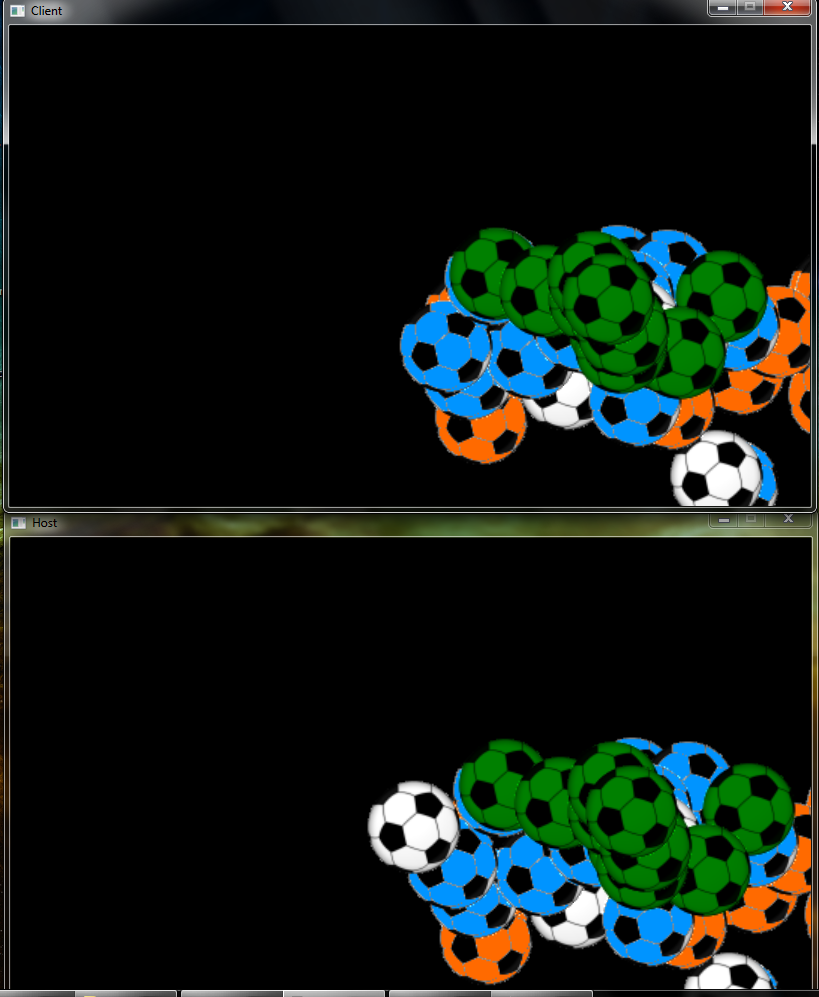
\includegraphics[width=8cm]{Pics/Networked_balls.png}
\end{center}
\caption{Networking sample}
\label{fig:networking_sample}
\end{figure}

The prototype is currently working. Figure \ref{fig:networking_sample} shows the bouncing balls sample in action, where we see that blue balls are generated by the client input, the red balls are generated by the host input, and the white balls are generated by the host script. % Figure [] shows the asteroid shooter sample where multiple ships cooperate in destroying falling asteroids.

%We have also studied some benchmarks on the two prototypes. The benchmarks show the bandwidth used by the samples with and without incremental transfers and local prediction, and they also show the average latency with and without lag compensation techniques.


\section{Future work}
Networking in Casanova is part of an appendix rather than the main work mainly because it is still incomplete. The implementation of the networking framework is still underway, and there is still not enough data to draw some conclusions and perform comparisons with other systems. Networking still requires an in-depth study of how to perform faster exploration of the game world with reflection (as discussed in Chapter \ref{chap:implementation}). Also, further optimizations such as updating some fields upon local update only, probabilistic updates from the host that take into account expected reliability of transmission to estimate which clients need what data, and a tracking server to move networked games on the Internet instead of limiting ourselves to local networks are being worked on.
 

\chapter{A General-purpose AI for Casanova}
\label{chap:goap}
A general AI for games is difficult to build. This difficulty stems from the fact that game AIs have different requirements, from very tight performance constraints, to the ability to deal with rapidly changing situations, and even to the need of looking smart and challenging while at the same time being beatable by the player. 

Current technology is such that most non-playing characters are little more than "animated wallflowers", with the inability to autonomously engage the player or achieve their own goals.

We believe that there is now the opportunity to create simulations of realistic agents showing complex and unpredictable (though always reasonable) behaviors through Goal Oriented Action Planning. We believe GOAP to be a general-purpose technique that enables agents that, while being smart enough to deal with in-game situations in unpredictable ways, can still be controlled by setting their goals as the designer wishes.

In the remainder of the appendix we show how we have used Goal Oriented Action Planning (GOAP) \cite{APPENDIX_C_GOAP_BOOK} to create agents that exhibit rational-looking planning. GOAP is a planning architecture designed for controlling autonomous characters in games, originally used in games for F.E.A.R. by Monolith Productions \cite{APPENDIX_C_GOAP_FEAR} but coming from the even older work STRIPS \cite{APPENDIX_C_STRIPS}. 

GOAP presents some important challenges when applied to more than a very small set of actions to be planned, given the combinatorial explosion of the search space of the main algorithm. Our main contribution is to show how the use of a layered system of GOAP planners (which we have aptly named LGOAP) can give rise to coherent plans that span long periods of game time, and which effectively plan dozens of actions for reaching the final goal. We also discuss how modifications can be added to this basic LGOAP in order to enable agents to learn from their environment, deal with incorrect assumptions, refine subsequent planning sessions and enable the emergence (and active planning) of cooperative behaviors.


\section{Activities}
\label{sec:activities}

The virtual world contains a series of objects. Objects are the backbone of the simulation, since they define the set of available actions for a user. An object is defined as a location, its available activities, and the agents that are using it at the moment.

The location of the object is, of course, where it is (at the moment: some objects may move, such as trains, bikes, groceries, etc.). The activities of an object are a series of actions that may be performed by an agent. For example, if a certain workplace only opens between 08:00 and 17:00 for its workers, but cleaners may clean it in the evening, then we may have the following activities:

\begin{lstlisting}
{ (work,(mon,08:00,9h),(tue,08:00,9h),...)
  (clean,(mon,18:00,2h),(tue,18:00,2h),...) }
\end{lstlisting}

Activities have preconditions and consequences. Preconditions are defined as a series of predicates that must be verified in order to perform the action; the agent will have to build plans such that each precondition is met before performing the desired action. Preconditions may be about the agent statistics, location, or certificates. Example preconditions for performing the work action at the office may be:

\begin{lstlisting}
health is good; works at office; is at office
\end{lstlisting}

Post-conditions represent changes to the agent statistics or certificates. For example, the work activity may leave the agent with more money, but also more stressed, hungry, and tired:

\begin{lstlisting}
money := money + 100,stress := stress + 0.1,
hunger := hunger - 0.2,sleep := sleep - 0.1
\end{lstlisting}


\section{Agent stats}
\label{sec:agent_stats}

An agent is modeled after the traditional BDI paradigm of beliefs, desires, and intentions \cite{APPENDIX_C_BDI}. The \textit{beliefs} of an agent mirror the agent's understanding of the consequences of an action, particularly with regard to expected costs and benefits. Scenarios that require learning can be built such that the agent plans are non-optimal because of wrong beliefs. An agent \textit{desires} to maximize his happiness and well-being, while minimizing the costs associated with doing so. Happiness is defined by the system designer, and can include anything ranging from prolonged survival, to performing certain actions, or reaching a goal. The agent's \textit{intentions} are represented by his planned sequence of future actions. Intentions may be dynamically adapted and revised in order to react to a changing scenarios.

In this section we mostly discuss the desires of the agent as represented by a series of internal statistics. Beliefs are discussed in Section \ref{sec:learning}, since beliefs are represented by the agent's learned responses of the environment. Intentions are discussed in Section \ref{sec:naive_goap}, since planning and then executing one's plan is the very definition of having intentions.

Formally, an agent is defined as a location, statistics, and certificates:

\begin{lstlisting}
<agent> ::= <location>,<stats>,<certs>
\end{lstlisting}

Location simply defines where the character is located in the virtual world, that is his current \texttt{x} and \texttt{y} coordinates. Statistics define a series of internal values that change as the character performs actions, and which represent a continuous description of the general status of the agent. A statistic is defined as a value, a series of thresholds, and a series of responses. The value is simply a number between 0 and 1 that represents for example how hungry the character is, with 0 meaning starved and 1 meaning full. Agents are not all the same, and have different thresholds of attention for each statistic, and also different costs and benefits obtained from performing certain activities. Thresholds are used to transform the continuous value of statistics into discrete predicates which are then used by the planner. For example, a user who gets hungry easily may define his thresholds to hunger as:

\begin{lstlisting}
{ 95% $\rightarrow$ good; 50% $\rightarrow$ ok; 25% $\rightarrow$ bad }
\end{lstlisting}

Responses represent how much more (or less) than the agents' standard responses an agent obtains benefits or incurs penalties when performing an activity. For example, an agent who dislikes working in general but who likes working as a teacher could have responses for the \texttt{stress} statistic such as:

\begin{lstlisting}
{ work $\rightarrow$ 200%; work.teach $\rightarrow$ 25% }
\end{lstlisting}

The above means that if the agent is merely performing some work, then he will suffer twice the stress of a regular character, but if he teaches then his stress will go as low as one-quarter of the default amount. Of course having a stress statistic and a work activity is just an example, since stats and activities are highly dependent on the simulation. 

Responses and thresholds may radically change how an agent plans. Plans will always be correct, in that if a plan exists such that it allows the agent to reach the goal then the planner will find it; the planner though will first explore those plans that are "liked" by the agent, and so thresholds and responses may change the solution found.

Finally, certificates are a series of tokens that represent ownership of virtual objects, such as weapons, a home, money, etc. Some activities require that the agent owns the appropriate certificate in order to be performed, and the planner will have to take care of planning the actions to obtain a given certificate before performing the actions that require it. For example, eating may require the ownership of food, working may require having a job, traveling to a distant star-system may require knowledge of the right warp coordinates, and so on.

Agents represent their social relationships as a series of additional statistics, one for every other agent to model a relationship with; an agent may also have certificates that represent special relationships such as \texttt{married to}, \texttt{boss of}, and so on which define discrete modifiers for certain social interactions.


\section{Naïve GOAP}
\label{sec:naive_goap}

We start with a description of the naïve version of the GOAP algorithm. The algorithm requires only a queue of partially explored action plans that are expanded by adding available actions to them until a plan that satisfies the original goals is found. An action is only added to the working queue when the previous actions in the queue verify its preconditions. Satisfactory plans are then added to the solutions queue, which is then used to extract the best plan at the end of the algorithm. The algorithm in pseudo-ML could be described as:

\begin{lstlisting}
compute_best_plan() =
  Q = [a | a <- empty_plan.next_available_actions()]
  S = []
  while Q <> [] do
    plan = Q.dequeue()
    if plan.satisfies_goal() then
      S.add plan
    else
      for a in plan.next_available_actions() do
        Q.enqueue(a::plan)
  if S = [] then
    return null
  else
    return S.dequeue()
\end{lstlisting}

The queue \texttt{S} stores solutions in decreasing order according to a metric that represents the (expected) distance from the final goals. If the actions monotonically decrease the distance from the goals, then we can sort solutions in \texttt{Q} according to distance from the goals, and the algorithm can simply return the first solution it encounters:

\begin{lstlisting}
compute_best_plan() =
  Q = [a | a <- empty_plan.next_available_actions()]
  while Q <> [] do
    plan = Q.dequeue()
    if plan.satisfies_goal() then
      return plan
    else
      for a in plan.next_available_actions() do
        Q.enqueue(a::plan)
  return null
\end{lstlisting}

In our case though, we do not have a definite goal except the maximization of stats. This means that a reasonable metric could simply be the cost-to-benefit ratio:

\begin{lstlisting}
plan.value() =
  benefit = mul [a.benefit() | a <- plan]
  cost    = mul [a.cost() | a <- plan]
  benefit / cost
\end{lstlisting}

The benefit of an action is computed as the weighted sum of all the stats that increase as a consequence of that action, while the cost is computed as the weighted sum of all the stats that decrease times the duration of the action. Notice that instead of multiplying costs and benefits, which would yield approximation errors, we use a log-sum to increase numerical precision.


\section{Heuristic pruning}
\label{sec:heuristic_pruning}

The complexity of the algorithm as described above is very high; if we have a maximum number $N$ of actions that we are planning for, or if we know that there is a satisfactory plan of $N$ actions, the complexity is $O(N^k)$ where $k$ is the number of available actions at each step. Planning for the long term may require dozens or even hundreds of actions, and the resulting search space would simply be too big to be explored in real-time.

Just like human beings do not consider absurd plans, though, plans that only accumulate actions with very high costs and no benefits at all after many actions do not really need to be considered. For this reason, before adding a new plan into the queue we check if it is reasonable according to a heuristic that removes plans that are either deadly or which have an excessive cost. Deadly plans are defined as those plans that take one or more statistics below the death threshold, for example because of starvation. Excessively costly plans are defined as those that take more than a certain number of actions \texttt{M} (to avoid pruning too early) and which value is smaller than a minimum value $\epsilon$:

\begin{lstlisting}
plan.reasonable() =
  cost    = mul [a.cost() | a <- plan]
  return not_dead(self.stats + cost) && 
        (plan.length <= M || plan.value() > $\epsilon$)
\end{lstlisting}

This way even though we risk pruning some plans that incur too many costs in the beginning, we greatly reduce the size of the plan space by removing plans that feature only travel or pointlessly long repetitions of costly actions. Also, we may explicitly prune plans that "run in circles", that is we may add a boredom stat to agents such that agents refuse to consider plans that require very long sequences of "uninteresting" actions. This trims loops and other useless plans on which the planner would waste a lot of exploration effort.


\section{Acting out plans}
\label{sec:enacting_plans}

After planning, we define how a character follows his plan. A plan is a sequence of actions, where each action has certain requirements. During planning we assumed the consequences of our actions to be predictable, so that we could put the actions in the right sequence to unlock the requirements for desirable future actions with past actions. Unfortunately planning cannot foresee perfectly what the responses of the world will be (unless the simulation is completely deterministic and there are no other agents), and so the same conditions that must be verified for planning are verified before (and in some cases during) the execution of every action. When an action preconditions are not met, then the planner is run again in order to create a new plan that takes into account the unexpected situation. Also, by storing the expected costs and benefits (or a likely range of values) of each action in the plan then we can compare this estimate with the actual results; when the actual results are outside the expected values, both too bad and too good, we trigger a new planning phase to avoid acting out plans that were too optimistic, and thus may lead to bad consequences, or too pessimistic and thus wasteful.


\section{Layered GOAP}
\label{sec:layered_goap}

The goals of our agents are long-term. To give our characters the ability to correctly plan for the long term we must be able to reduce the search space far more than what can be done with simple heuristics: the longer the plans, the harder it gets to efficiently find plans or (perhaps as importantly) to stop searching when no adequate plan is found. Moreover, aggressive pruning often forces the agent into local minima. To address the problem, we have built a framework that combines multiple layers of GOAP, which we have christened LGOAP (Layered GOAP); each layer restricts the search space for successive layers, but plans at a lower granularity. The system may use as many higher-level layers for planning up to (virtual) months or years ahead as needed. Each layer creates a plan roughly of the same size as more precise layers, but it covers a different time span. The last layer plans precise actions in detail, but only for a very short time-span (it may be a few hours in a simulation, or it may be a few minutes in a game where the scenario changes in real-time very quickly such as a fighting game or a shooter). Similar hierarchical approaches have been seen in computer graphics \cite{APPENDIX_C_CLIPMAPS}, path-finding \cite{APPENDIX_C_HIERARCHICAL_PATHFINDING}, and even AI itself \cite{APPENDIX_C_HIERARCHICAL_AI}.

This means that the full planner is defined as a series of layers. The first layer plans for the longest span of time, while successive layers recursively refine its plan until finally then $n$-th layer (the last one) finds the concrete plan. Each layer contains an instance of the GOAP algorithm and a time-span for which to build the plan. Layers successive to the first also have a series of constraints that come from the previous layer(s); constraints are a pair in the form of an overall goal for the plan, and a series of allowed action-sets to which the search is restricted for the various time slots. A goal is simply a series of weights that are used to compute the benefit and the cost of an action. An example four-layered architecture is shown in Figure \ref{fig:layers}; the first layer compute the steps until the final goal, but each step cannot be acted out directly and requires more planning; the second and third layers computes the steps that cover only part of the overall plan, but these steps are more specific and realize multiple steps of the overall plan; the final layer computes the actual sequence of actions that the agent performs, but these actions only cover a short time span. Fortunately, the short time span of the concrete planner are coherent with the overall plan thanks to the layered system.

\begin{figure}
\begin{center}
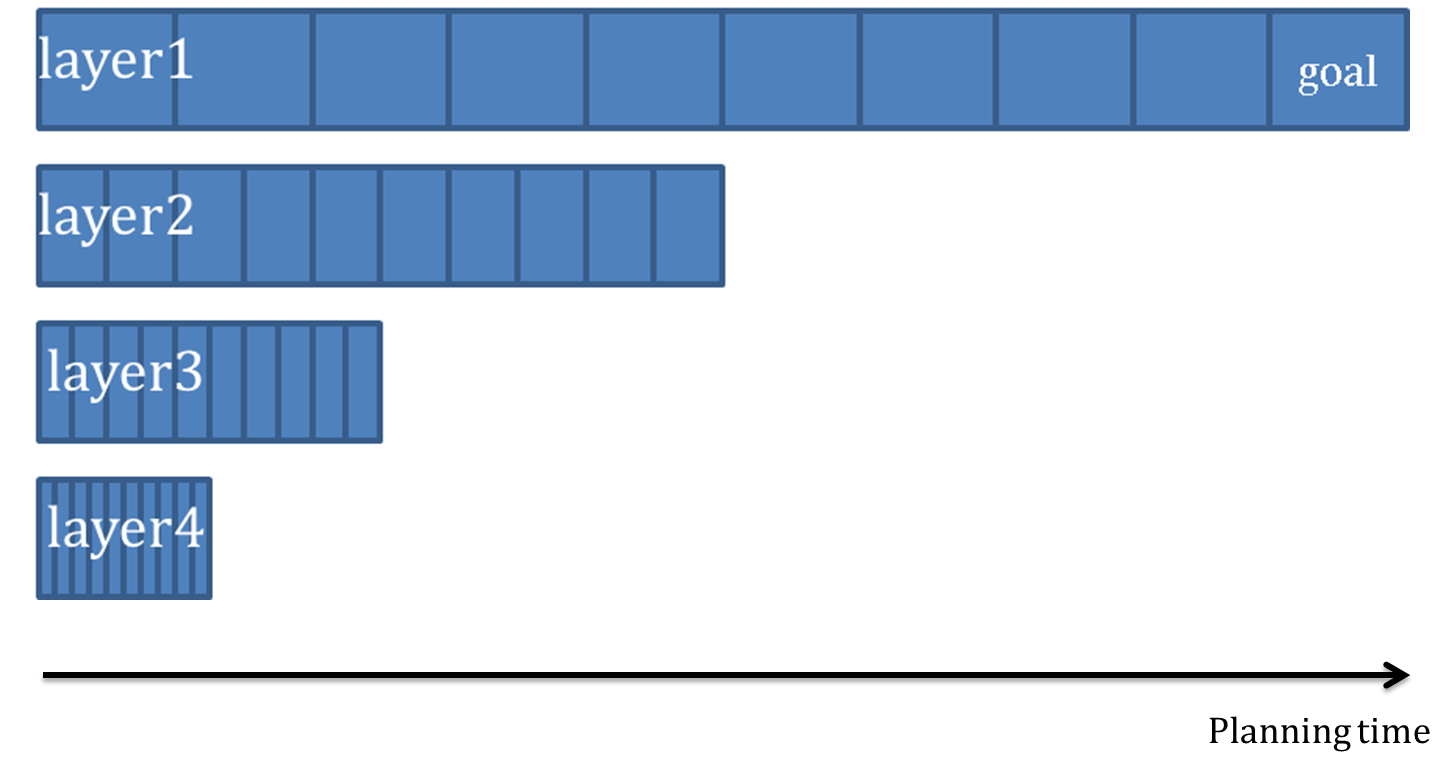
\includegraphics[scale=0.3]{Pics/layers.png}
\end{center}
\caption{Four layers planner}
\label{fig:layers}
\end{figure}  

Higher layers thus do not plan in detail; they simply plan a series of requirements that successive layers must take into account when performing their planning. Requirements steer the planning by modifying the weight of certain statistics, in order to make the planner more aware of certain statistics that change. For example, if the weights from a previous planner are:

\begin{lstlisting}
<money=0>,<food=0.1>,<stress=3.0>
\end{lstlisting}

Then an action plan that makes the character spend a lot of money but decrease his stress level a lot will be perfectly acceptable, since the higher-level planner has instructed successive layers to ignore the costs associated with decreasing the amount of money. We can refine our model further by specifying two different weights, one for the benefits and one for the costs.

This way we are still accepting plans that increase money or reduce hunger, but if we get a chance to decrease stress at the expense of either hunger or money then the plan will have a very high score. Weights are determined because the actions that the higher-level planner decides for can yield a wide range of benefits, but the planner will decide exactly what benefits are relevant and which actions are allowed only because they may be needed by the lower-level planners to create a working plan.

Higher-level planners also have the chance to restrict the set of available actions for successive plans. This restriction states the sets of allowed actions for each time slot, so that successive planners will have to restrict their search to combinations of these actions. For example it may be reasonable to have the following block of actions:

\begin{lstlisting}
walk,take-bus,drive,take-train,work,eat,chat
\end{lstlisting}

The lower-level planner can then combine them in a sequence where the user walks to the bus station, then takes the bus, then walks to work, then does his workday, and then leaves work:

\begin{lstlisting}
walk,take-bus,walk,work,chat,work,eat,
work,chat,work,walk,take-bus,walk
\end{lstlisting}

All these restrictions are actions that are designed by hand for the appropriate layer. When a planner cannot find a working plan that supports the requirements of the higher-level plan, then the higher-level layer re-plans by taking into account the new situation it has to plan from.


\section{Learning Expected Costs and Benefits}
\label{sec:learning}

The simulation is intended to be partially unpredictable, in order to provide unexpected situations to the agents. For example, the \texttt{take-train} activity may have probabilistic pre-conditions that represent the fact that the train may be late; also, the train may not take any more passengers if more than 100 people have boarded it already. The pre-conditions for taking the train may then be:

\begin{lstlisting}
money > 10,p > 0.99, passengers < 100
\end{lstlisting}

Surprises then \textit{emerge} from the simulation, for example traffic jams or trains and buses that are too full, thereby creating unpredictable situations that should be learned by the agents in order to obtain a more effective behavior.

To make agents resilient to change, we give them the ability to learn. Learning means that an agent stores a table of statistical models for actions in general, and for the same actions when performed with specific conditions (such as time or location). These statistical models store some distribution of the expected results of actions, in order to be able to better estimate the most likely range of the benefit and cost of an action for accurate planning. A very simple estimator for learning costs and benefits simply records the actual cost and benefit of an action and stores them in a rolling average and variance:

\begin{lstlisting}
avg' = $\alpha$ * x + (1.0 - $\alpha$) * avg
var' = $\alpha$ * (x - avg) * (x - avg') + (1.0 - $\alpha$) * var
\end{lstlisting}

More complex estimators could use a wealth of traditional statistical and machine learning techniques such as \cite{APPENDIX_C_REINFORCEMENT_LEARNING,APPENDIX_C_STATISTICAL_PATTERN_RECOGNITION}, etc.

With this new definition, agents can learn that an apparently valid action that often incurs in a penalty should be recorded as having a higher cost than expected, since it has a bigger chance of failing. For example, an agent who often arrives among the last agents to board a full train can learn that this specific train, only for him, does not yield the expected benefit. He may then plan to board a different train at a different time, or to use some other means of transportation. 

Similarly, we can define agents that model no-knowledge in terms of worst- (or best-) case scenarios, creating initial tentative plans that are then tried and refined while learning useful notions for re-planning.

The learning system means that while planning, each action yields a \textit{range} of expected results. This means that we have cost and benefit as the two ranges respectively $c_l, c_u$ for the cost and $b_l, b_u$ for the benefit. We have multiple ways to combine these ranges into a ratio: \textit{(i)} the pessimist algorithm simply takes the worst-case ratio of $\frac{b_l}{c_u}$ of the lowest benefit and the greatest cost; \textit{(ii)} the optimist algorithm takes the best-case ratio of $\frac{b_u}{c_l}$; \textit{(iii)} the average algorithm takes the average ratio of $\frac{b_{avg}}{c_{avg}}$, where $b_{avg} = \frac{b_u+b_l}{2}$ (and similarly for the cost); and \textit{(iv)} the distribution algorithm that maintains the joint distribution of costs and benefits in case we used some form of statistical learning technique, or to merge intervals in a new interval that uses \textit{(i)} and \textit{(ii)} as its bounds.


\subsection{Learning Whole Plans}
Our framework supports agents capable of forming habits by storing whole plans that they executed in the past. When a plan is built and performed, then we compare its expected benefits with the actual benefits. We discard plans that do not have a sufficiently high reliability, that is even if a plan performs great but in an unexpected way (that is within more than a $\delta$ value within the expected gains or losses) then we will not save this as a good plan; of course we still use our new knowledge as described above to steer the planner towards the actions of this plan, but the \textit{whole} plan is not considered successful. We maintain a working memory of old, successful plans with their associated resulting benefits. Before planning for a certain set of goals and limitations, we check the working memory to find the best known plan that realizes the goals and stays within the required limitations as dictated by the higher-level layers. If there is one or more plans that fill these needs, then we pick the best one and we skip the whole planning phase, otherwise we plan as usual. Since planning is done in real-time, this gives us agents that can create habits through which they get much faster planning whenever they can avoid re-thinking the same plan.

After an old plan is executed then we can compute a rolling average (or some other, more accurate estimation) of its reliability; this gives us a way to maintain the reliability of plans in a changing environments. It is important to pick a technique that does not suffer too much from the presence of a rare occurrence (which should be treated as statistical noise), but which is capable of adapting to trends in the game world events.


\subsection{Learning and Layers}
Higher-level plans need a way to specify the sets of actions allowed for a certain time block, in order to give freedom to the lower-level planners to combine these allowed actions sets into more specific sequences. The action-sets may be designed by those who build the concrete system, but doing so risks forcing the system to behave along some predefined "rails" when the action-sets are not expressive enough. If this happens, then the higher-level layers would be too much constrained, and they would not be able to reach good plans, but instead they would force the lower-level layers along their same constraints and sub-optimal strategies. Alternatively, we can let the system sort out the most useful action-sets by storing the actions that happen together most often. This amounts to an ulterior form of learning, since the agents will learn how to plan at a higher-level; moreover, this makes it possible to have characters who start by only planning for a few days at a time, but who gradually learn how to plan for a longer time-span.


\subsection{Implicit Social Interactions}
The learning system steers social interactions because as actions are performed, the learning abilities of an agent learn the \textit{social consequences} of the various actions. For example, an agent may learn that since another agent he likes is often present at work on Monday morning, then Monday mornings are learned to also give a boost to social interactions for no additional costs. This steers the planner towards going to work at that time slot even if it may be possible to do so at other times, because going to work in that time slot is also beneficial to social interactions. Social interactions may also make a character avoid performing actions in certain places and at certain times because doing so would be learned to be associated with meeting disliked agents that would then result in a cost for the social statistics.

To represent social relationships, a matrix of each pair of agents is maintained by the system. The matrix, which is sparse because many agents do not know each other, contains the relationship between two agents. The relationship between agents is an \textit{index} that goes from -1 (dislike), through 0 (neutral), to 1 (like). The relationship index is used to compute a multiplier for the social costs or benefits of an action. Characters automatically develop a social index by performing actions together and in vicinity. The initial social compatibility can be determined by a function on the agents personal attributes, which are their tolerance thresholds and their responses from their environment, or by different forms of defining an agent profile. Social compatibility may be defined as similarity or dissimilarity, and may even be defined by an initial randomization of likes and dislikes among agents.


\subsection{Explicit Social Interactions}
When characters like each other enough, that is more than a certain threshold, then they may choose to do some social activity together. The social activity is added to the higher-level planner at a slot that is compatible for both agents. Compatibility is measured as a positive weight for social interactions (that is in that slot it is desirable to have social interactions), and expected geographical distance. If the social interaction fails, then the relationship index is decreased; in case of a successful meeting, on the other hand, the relationship index is increased significantly.


\section{Assessment}
\label{sec:assessment}

To test our system, we devised a case study that offers a challenging environment for our agents. The system is still under construction and it is currently missing some important features, in particular learning and social actions. The most relevant part of our method though, layered planning, has been implemented and put to the test with satisfactory results.

In our game (depicted in Figure \ref{fig:case-study}) a pirate ship has to leave the pirate lair to raid the surrounding planets. These planets have different strengths and yield a different reward (loot). Not all planets can be reached right away: before traveling through some planets the ship needs to raid other planets that contain star charts required to reach the goal. The case to be solved is constructed in such a way that the ship will have to go back to the pirate lair to repair and upgrade as it progresses, and will have to refuel frequently at an ulterior location.

\begin{figure}
\begin{center}
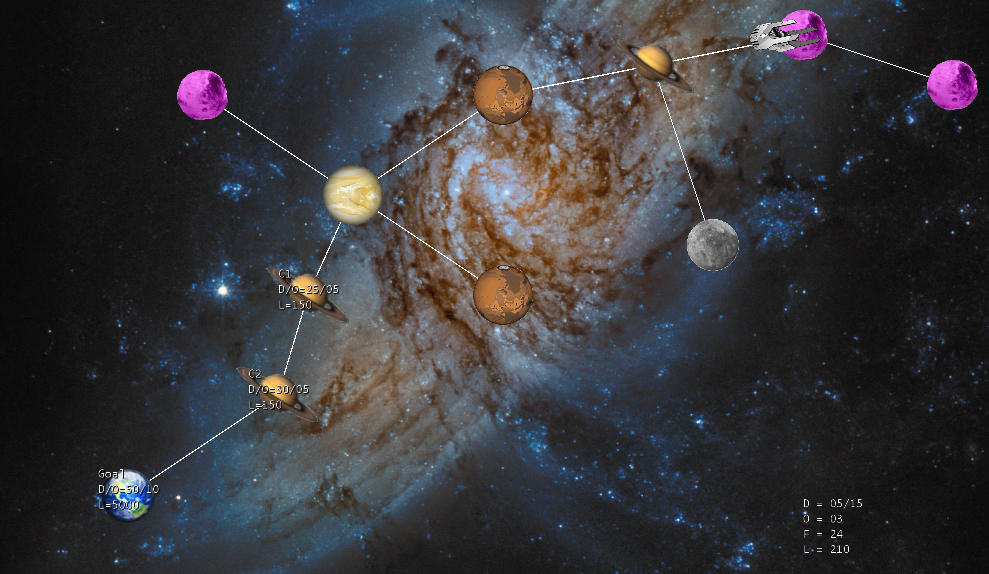
\includegraphics[scale=0.3]{Pics/Middle.png}
\end{center}
\caption{Case study}
\label{fig:case-study}
\end{figure}  

The actions available to our pirate ship are \texttt{move}, \texttt{raid}, \texttt{repair}, \texttt{upgrade}, and \texttt{refuel}. The number of actions for a plan that can reach the goal are approximately $100$, even for such a deceptively simple scenario, yielding a search space of approximately $100^5$ possible plans, given that at every step there are on average $5$ available actions that may be taken next. We have tested successfully more difficult scenarios that require even more overall actions because of the higher number of planets arranged in a much-larger grid, but we believe that the case presented here is already sufficiently challenging.

Each action has strict requirements, such as having enough fuel and the required star charts for moving to a planet, having enough loot to upgrade and so on. This still leaves many exploration options intact though, especially with regard to when to refuel, repair, and upgrade.

The current system uses two layers. The first layer plans the order in which to attack the most important planets (refueling stations and star chart owners), and the required upgrades that are needed in order to attack those planets when they are too powerful for the ship. The second layer realizes these plans to obtain these goals in the required order.

The performance of the planner is such that it is possible to perform planning in real-time. Plans are computed in less than one frame (at 60 frame per second) on a 1.8Ghz Intel Core Duo, given that plans compute few actions at a time thanks to the layering system.

The scenario offered in our case study is challenging because to reach the goal there is no single monotonically increasing stat or utility value that the ship can use to steer itself. Additionally most of the stats change in a chaotic fashion during the execution of a successful plan. Although keeping these stats high may appear desirable (for example health, fuel and loot) sometimes these must be sacrificed for long periods of time in order to reach well-defended, distant planets.
  
\begin{figure}
\begin{center}
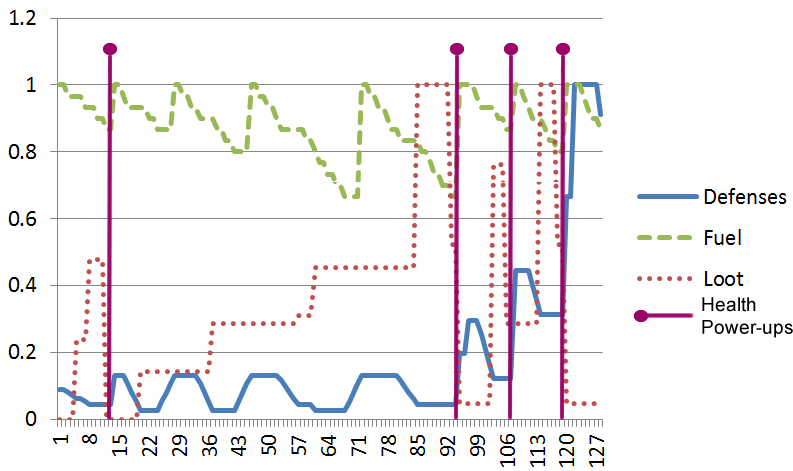
\includegraphics[scale=0.3]{Pics/graph1-stats.png}
\end{center}
\caption{Ship stats}
\label{fig:graph1-stats}
\end{figure}  

In Figure \ref{fig:graph1-stats}, it is possible to see the graph of the different stats associated with the spaceship during the simulation. The health ("Defenses") and fuel stats are continuously sacrificed to reach planets and do battle; defenses also gradually increase as the pirate ship performs upgrades ("Health power-ups"), as evidenced with the dotted vertical lines. Loot is accumulated but also spent in order to buy power ups. The first and third power ups are single, while the second and fourth are double and thus yield an even stronger increase in statistics.

\begin{figure}
\begin{center}
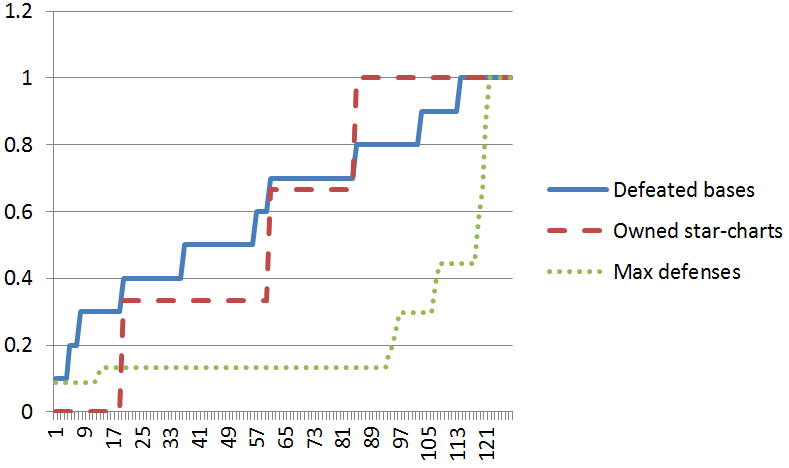
\includegraphics[scale=0.3]{Pics/graph2-goals.png}
\end{center}
\caption{Ship goals}
\label{fig:graph2-goals}
\end{figure}  
  
In Figure \ref{fig:graph2-goals}, it is possible to see the global goals, as achieved by the higher-level layer. This layer is the one responsible for planning long-term actions, and in fact we can see that the number of defeated bases, the number of owned star charts, and the defensive abilities of the ship are increased monotonically. Most notably, the success in achieving global goals is quite slow, and many actions could easily but wrongly be classified as useless by other AI systems since they do not yield a visible global advantages but they yield significant immediate disadvantages.

Finally, by lowering or increasing the agent thresholds we generate plans that are still valid (those that kill the ship are always rejected), but where the ship is ruthless and aggressive and accepts to remain damaged and under-fueled for long periods of time, or very conservative and repairing and refueling very often.

As a final loose note it is interesting to observe that the resulting behavioral pattern is very similar to that of a human player playing an RPG game, where the player alternates exploration/combat sessions with resting sessions at the closest town. The very same behavior automatically emerges from our system, thereby giving us added confidence in the quality of the technique, since we did not give any hints whatsoever that this was the desired result, instead letting the system deduce its usefulness.


\section{Missing and implemented}
\label{sec:discussion}

Our system will be extended with two major additions that we were unable to implement in time for this work: learning and adaptive planning and social interactions between agents. Learning would equip our agents with the ability to adjust their planning by including feedback from the execution of earlier plans, thereby creating an adaptive planning system able to deal with incomplete knowledge. Layers themselves could be learned, for example by finding common sequences of actions that occur often in lower-level layers that can then be grouped and considered a single action. Social interactions would make it possible for our agents to plan actions to perform together when it is advantageous to do so. Such interactions could also include coordinating group actions such as team fighting. Such a social framework could also make use of a layering system for handling groups of agents that must each behave reasonably but in a coordinated fashion. Additionally the ability to mix this planner with more traditional control structures for AIs, such as decision trees, neural networks, finite state machines, etc. would make it possible to have agents capable of more convincing local reactions to unexpected situations, such as a "fight-or-flight" reflex that does not leave the agent vulnerable to immediate dangers while planning for a full response.

Last bu not least, as soon as the planner reaches a definitive shape it will be added to Casanova in the form of a library, an extension to the language, or both.


\chapter{Casanova and Data-bases}
\footnotetext{This chapter is partially derived from the paper \cite{CASANOVA_SEBD}.}
\label{chap:casanova_and_dbs}
In this appendix we present a novel observation: many game development problems may be already solved in a field which, at a first glance, may appear utterly unrelated: databases. The field of databases already contains a large body of relevant research works which simply needs to be studied and adopted by game developers. Casanova indeed draws much inspiration from modern database systems and tries to apply some of their wisdom to game making. The language aims at offering a series of abstractions and optimizations that allow a developer to specify only certain core aspects of a game logic and visualization, without concerning himself too much with boilerplate code such as state traversal or query optimizations, exactly in the spirit of a modern relational DBMS.

Interestingly enough, Casanova is not alone in its effort. There is at least one other research effort of linking database research with game development; this work has yielded the SGL language \cite{SGL}, an experimental game development language which uses SQL queries to define the way the various entities of the game world are updated at each time-step of the simulation. SGL may be unsuitable for larger scale problems, since it offers no techniques to model the game world and entities, but the underlying optimizations and expressivity of the framework are undeniably powerful and require virtually no effort on the part of the game developer in order to obtain important speedups.


\section{The Game World}
The logical simulation of a game starts at the first step of the creation of a new database: modeling (or conceptual schema definition). A game consists, at its core, of a series of concepts and their relationships. These describe the semantics of a game world and represent a series of assertions about its nature. Specifically, these concepts describe the things of significance to the game, about which we are inclined to collect information, and characteristics of (attributes) and associations between pairs of those entities (relationships). Most entities are in the plural, and thus require being stored in tables or collections.

After defining the data model of the game world, game developers must define the dynamics of the game, that is how each game entity is updated at every tick of the game loop. The game dynamics are, at the core, a series of rules that define how each entity (or, better, each attribute of each entity) is updated during each tick. A major point of difference between games and databases lies in the frequency of the dynamics of the system: the game world is updated about once every sixtieth of a second to achieve a smooth simulation, instead of waiting for user-initiated events; indeed, a large number of changes in the game world are entirely automated and occur even without direct user interaction over time, for example because of physics or AI.

Some of the game dynamics simply require to update "small" values, such as a position and a velocity from a velocity and acceleration respectively. Other game dynamics require more sophistication. For example, rules may be used to populate lists or other composite data-structures according to complex, deeply nested computations.

Certain attributes of a Casanova game entities store "pointers" to other game entities. These attributes are marked as \texttt{ref}, thereby representing referential constraints (foreign keys) \cite{DATABASE_SYSTEM_IMPLEMENTATION} between different entities; with references we define attributes which contents are not to be updated during a tick.

Rules are treated as transactional operations \cite{APPENDIX_D_11} in order to ensure the consistency of the game world. This means that all rules are evaluated on the game world at a certain time-step and then all their results are written, at the same time, into the new game world. This way all rules behave in a predictable way and no rule ever "sees" the game world halfway between different ticks of the simulation. Moreover, this enables a very important optimization: evaluating rules in parallel with different threads so as to speed up the simulation, thus freeing computational power to animate more entities or use more complex algorithms.

Rules that recompute lists or collections also present an additional optimization opportunity on operations that compute a Cartesian product between two lists, which if it were naïvely computed would have quadratic complexity. By using optimization techniques such as a hash-join or similar the complexity becomes much lower. Our benchmarks \cite{APPENDIX_D_7} suggest improvements of an order of magnitude in the run-time efficiency of the entire simulation when applying query optimization techniques. Moreover, this process of optimization could be entirely optimized, whereas game developers still write such faster algorithms by hand every time they encounter the problem \cite{APPENDIX_D_HANDMADE_OPTIMIZATION_IN_GAMES}.

Rules and queries are not always the best abstraction to represent the way a game world evolves itself over time. For this reason we have added to Casanova a scripting system, which is decidedly akin to a system of triggers and stored procedures (where triggers may also be timers or user actions).


\section{Persistency, Saving Games \\ and Multiplayer Games}
A game world requires some persistency. Persistency comes into play both in single-player games and multi-player games. Single-player games require persistency because the overall playing experience of a game takes longer than a single play session, and so the game state requires serialization on persistent memory. This process, known as \textit{save and load} allows a player to suspend the current state of the game on disk, in order to be able to resume playing the game later without losing his progress.

A more complex case where the game world is persistent is that of multiplayer games. Multiplayer games have two different sets of problems to tackle: \textit{(i)} synchronizing the game world in real-time between different clients; and \textit{(ii)} reliably storing a persistent world and all the players’ data.

Synchronization of the game world between many clients and the game server (or host) must happen in real-time, but each client needs a responsive experience. For this reason most modern games employ client-side prediction and lag-compensation algorithms \cite{APPENDIX_B_LATENCY_COMPENSATION}, that is all operations that need to modify the host’ game world but which are initiated locally by a client always appear to succeed on the client but are instead sent to and then validated by the host. This amounts to a form of eventual consistency \cite{APPENDIX_B_EVENTUAL_CONSISTENCY}, given that temporary misalignment is tolerated between host and client, but we offer guarantees that \textit{eventually} such a misalignment will be fixed by the system.

The problem of storing a persistent, huge world for many players (massively multiplayer games such as EVE or World of Warcraft feature up to tens of thousands of concurrent active players) requires hybrid in-memory/on-disk databases with very quick access and supporting up to hundreds of thousands of concurrent accesses. To reduce the scope of these technical challenges the game world is sometimes segmented into different copies of the world, grouping players by geographical region, but other games such as EVE Online feature different techniques such as a hierarchical structure of distributed servers to avoid segmentation and offer a single persistent game world.


% todo: write from the wiki pieces
\begin{comment}
\section{Match-making}
In multiplayer video games, matchmaking is the process of connecting players together for online play sessions.

TrueSkill is a Bayesian ranking algorithm developed by Microsoft Research and used in the Xbox matchmaking system built to address some perceived flaws in the Elo rating system. It is an extension of the Glicko rating system to multiplayer games.[1][2]

TrueSkill maintains a belief on the skill of each player; every time a player plays a game, the system accordingly changes the perceived skill of the player and acquires more confidence about this perception.

Published formulas for Trueskill are not complete, and some needed functions are simply shown as graphs. Some of the math is spelled out in the paper.

A player's skill is represented as a normal distribution  characterized by a mean value of  (mu, representing perceived skill) and a variance of  (sigma, representing how much "confidence" the system has in the player's  value). As such  can be interpreted as the probability that the player's "true" skill is .

On Xbox Live, players start with  and ;  always increases after a win and always decreases after a loss. The extent of actual updates depends on each player's  and on how "surprising" the outcome is to the system. Unbalanced games, for example, result in either negligible updates when the favorite wins, or huge updates when the favorite loses surprisingly.

Factor graphs are used to "pack up" each team into  pairs on which the update formulas are run; the skill updates are then correctly distributed to each player.

Player ranks are displayed as the conservative estimate of their skill, . This is conservative, because the system is 99\% sure that the player's skill is actually higher than what is displayed as their rank.

The system can be used with arbitrary scales, but Microsoft uses a scale from 0 to 50 for Xbox Live. Hence, players start with a rank of . This means that a new player's defeat results in a large sigma loss, which partially or completely compensates their mu loss. This explains why people may gain ranks from losses.

Another challenge that multiplayer games face is that of making use of the huge amount of data that can be gathered from players’ behavior through data-mining techniques. A common instance of this is the match-making problem \cite{APPENDIX_D_13}: given the preferences of the players who are currently waiting to start a game, determine the ideal group of players who all have similar skills, low-latency between each other, similar preferences, etc. Some games even feature team-play, and so the best teams must be found automatically.


\section{Gameplay balancing}
In game design, balance is the concept and the practice of tuning a game's rules, usually with the goal of preventing any of its component systems from being ineffective or otherwise undesirable when compared to their peers. An unbalanced system represents wasted development resources at the very least, and at worst can undermine the game's entire ruleset by making important roles or tasks impossible to perform.[1]

Balancing and fairness

Balancing does not necessarily mean making a game fair. This is particularly true of action games: Jaime Griesemer, design lead at Bungie, said in a lecture to other designers that "every fight in Halo is unfair".[2] This potential for unfairness creates uncertainty, leading to the tension and excitement that action games seek to deliver.[3][4][1]

In these cases balancing is instead the management of unfair scenarios, with the ultimate goal of ensuring that all of the strategies which the game intends to support are viable.[2] The extent to which those strategies are equal to one another defines the character of the game in question.

Simulation games can be balanced unfairly in order to be true to life. A wargame may cast the player into the role of a general who was defeated by an overwhelming force, and it is common for the abilities of teams in sports games to mirror those of the real-world teams they represent regardless of the implications for players who pick them.

[edit]Difficulty level

Digital games often allow players to influence their balance by offering a choice of "difficulty levels".[5] These affect how challenging the game is to play.

In addition to altering the game's rules, difficulty levels can be used to alter what content is presented to the player. This usually takes the form of adding or removing challenging location or events, but some games also change their narrative to reward players who play them on higher difficulty levels (Max Payne 2) or end early as punishment for playing on easy (Castlevania).

Difficulty selection is not always presented bluntly, particularly in competitive games where all players are affected equally and the standard "easy/hard" terminology no longer applies. Sometimes veiled language is used (Mario Kart offers "CC select"), while at other times there may be an array of granular settings instead of an overarching difficulty option.

An alternative approach to difficulty levels is catering to players of all abilities at the same time, a technique that has been called "subjective difficulty".[6] This requires a game to provide multiple solutions or routes, each offering challenges appropriate to players of different skill levels (Super Mario Galaxy, Sonic Generations).

Difficulty can also be managed by a third party or the game itself; see the Gamemaster section below.

[edit]Pacing

Balancing goals shift dramatically when players are contending with the game's environment and/or non-player characters. Such player versus environment games are usually balanced to tread the fine line of regularly challenging players' abilities without ever producing insurmountable or unfair obstacles.[4] This turns balancing into the management of dramatic structure,[3] generally referred to by game designers as "pacing".

Pacing is also a consideration in competitive games, but the autonomy of players makes it harder to control.

Similarly, game developers often need to understand the preferences of their players or if there are certain conditions in the game that favor certain players, in order to maintain a fun, balanced and fair experience for everyone. Discriminating useful patterns from previous games logs requires the ability to wade through huge data bases to make sense of their information. This can be achieved with data-mining techniques for the study of trajectories of data or clusters of user preferences.
\end{comment}
 

\chapter{Casanova in Other Languages}
\label{chap:casanova_in_haskell_and_cpp}
In this appendix, we discuss the conceptual prototypes that we used to define the Casanova semantic model. The ideas presented here could also be adapted in order to bring Casanova to other systems that feature similar meta-programming capabilities.

We start by introducing Haskell type classes \cite{APPENDIX_E_HASKELL_TYPE_CLASSES}, which we used to understand how to explore data-types inductively to generate functions. We then outline how we could have used those for implementing Casanova, a project that we never finalized in practice because of the lack of (as perceived by us) high quality gaming libraries for Haskell. We then discuss C++ partial template specialization \cite{APPENDIX_E_PARTIAL_TEMPLATE_SPECIALIZATION}, a meta-programming feature that we have used to build a working prototype of Casanova in C++, together with a sample game for testing purposes.

At a first glance, it may appear peculiar that C++ templates and Haskell type classes are lumped together in the same appendix. Interestingly though, there is evidence \cite{APPENDIX_E_TYPE_CLASSES_VS_TEMPLATES} that the expressive power of Haskell type classes may be matched by that of C++ templates with partial specialization. The biggest difference between the two may be that C++ templates do not offer a way to name the predicates that a type parameter must satisfy in order to be used in a given class (concepts \cite{APPENDIX_E_CONCEPTS} were proposed but then removed from the latest standard of the language). From our point of view this means that C++ offers a less constrained version of the same functionality, with more freedom to express complex patterns \footnote{without resorting to complex type-system hacks such as some auxiliary type predicates as used in \cite{APPENDIX_E_HLISTS} (which is a brilliant piece of work notwithstanding)}, but also with more problems associated to unforeseen interactions between different libraries.


\section{Haskell and type classes}
Type classes are constraints that are added to type variables in parametric polymorphic types. Such constraints are in the form \texttt{C a}, where \texttt{C} is a type class and \texttt{a} is a type variable. The constraint is such that all the operations that \texttt{C} defines must be supported by any type \texttt{a} that is used to instantiate the polymorphic type. This amounts to a form of ad-hoc polymorphism \cite{APPENDIX_E_AD_HOC_POLYMORPHISM}.

A very simple usage of type classes, and historically one of their first uses in the Haskell programming language, was that of implementing overloaded arithmetic and equality operators without recurring to ad-hoc implementations such as the "eqtypes" of Standard ML. Type classes are now used in many different contexts beyond their original uses \cite{APPENDIX_E_USES_OF_TYPE_CLASSES}.

\subsection{Overview}
A type class is defined as a set of function or constant declarations, in the form of name and type pairs. The type class then represents a set of actual types that all support \textit{at least} those functions and constants.

For example, we know that the equality class requires that a certain type supports the \texttt{(==)} equality operator. We define such class as:

\begin{lstlisting}
class Eq a where
  (==) :: a -> a -> Bool
\end{lstlisting}

We could define integers as belonging to the equality type class by instancing the type class on the integer data-type and providing an implementation for the equality operator that explicitly uses the integer equality function:

\begin{lstlisting}
instance Eq Integer where 
  x == y  =  integerEq x y
\end{lstlisting}

Type classes may also be used inductively; for example, given the definition for a binary tree, we may define equality for a tree in terms of the equality of its elements:

\begin{lstlisting}
instance (Eq a) => Eq (Tree a) where 
  Leaf a         == Leaf b          =  a == b
  (Branch l1 r1) == (Branch l2 r2)  =  (l1==l2) && (r1==r2)
  _              == _               =  False
\end{lstlisting}

This ability to define type classes for parametric types in terms of the same classes applied to their parameters proves crucial in implementing Casanova.


\subsection{Advanced uses}
Type classes may operate on types of any kind \footnote{In type theory, a kind is the type of a type constructor. A kind system is essentially a simply typed lambda calculus "one level up", endowed with a primitive type, denoted \texttt{*} and called "type", which is the kind of any data type. \cite{CHAPTER_1_PL_INFLUENCE_ON_PL}}, not just \texttt{*}. For example, the monad type class works on types of kind \texttt{* -> *}, such as \texttt{List}, \texttt{Maybe}, etc. which all expect exactly one type parameter:

\begin{lstlisting}
class Monad m where
  (>>=) :: m a -> (a -> m b) -> m b
  return :: a -> m a
\end{lstlisting}

Type classes can also be used with multiple type parameters, in order to define relations on types. For example, consider the definition of an algebraic multiplication system, where we want to support the following multiplication operations between matrices, vectors, and numbers:

\begin{lstlisting}[language=Haskell]
(*) :: Matrix -> Matrix -> Matrix
(*) :: Matrix -> Vector -> Vector
(*) :: Matrix -> Int -> Matrix
(*) :: Int -> Matrix -> Matrix
...
\end{lstlisting}

We may define a type class for this scenario as follows:

\begin{lstlisting}[language=Haskell]
class Mult a b c where
  (*) :: a -> b -> c
 
instance Mult Matrix Matrix Matrix where
  {- ... -}
 
instance Mult Matrix Vector Vector where
  {- ... -}
\end{lstlisting}

Unfortunately we are missing an important aspect of the multiplication operator: the third parameter \textit{is determined} by the first two, without ambiguity. We can state this in Haskell by specifying the dependencies between the type parameters:

\begin{lstlisting}[language=Haskell]
class Mult a b c | a b -> c where
  (*) :: a -> b -> c
\end{lstlisting}

Similarly, type families \cite{APPENDIX_E_TYPE_FAMILIES} allow us to define type-level computations that are performed at compile time. This may be used by a Casanova implementation to define the decorated version of the user-provided type for the game world with additional attributes for rendering, networking, etc.


\subsection{Casanova in Haskell, a sketch}
%Comparing Approaches to Generic Programming in Haskell, Ralf Hinze, Johan Jeuring, and Andres Löh

Casanova requires us to apply functions such as \texttt{update} and \texttt{draw} generically to all data types. This requires a uniform representation of data types. Except for basic predefined types such as \texttt{Float}, \texttt{IO}, and \texttt{->}, every data type can be viewed as a labeled sum of possibly labeled products \cite{APPENDIX_E_STRUCTURE_REPRESENTATION}. We can thus define a series of data-types for this encoding that distinguish between sums and products of types with the possible addition of labels:

\begin{lstlisting}
data a :+: b = Inl a | Inr b
data a :*: b = a :*: b
data Unit = Unit
data Con a = Con a
data Label a = Label a
\end{lstlisting}

Notice that in Haskell a type constructor may be in operator form, so the above has defined two new parametric data types which are named \texttt{:+:} and \texttt{:*:}. We can now define arbitrary data-types in terms of the above definitions; for example, we may write lists or trees as:

\begin{lstlisting}
type List' a = Con Unit :+: Con (a :*: (List a))
type Tree' a = Con Unit :+: 
               Con a :+: 
               Con (Tree a :*: (a :*: Tree a))
\end{lstlisting}

The set of types that can be defined with explicit structure-representation is isomorphic \cite{APPENDIX_E_STRUCTURE_REPRESENTATION} to the set of types, as witnessed by a so-called embedding-projection pair that is capable of converting values of a type into values of its structure-representation type and vice-versa. The embedding projection functions are the inverse of each other.

For example, for the List data type we can define the conversion functions as:

\begin{lstlisting}
fromList :: List a -> List' a
fromList Nil = Inl (Con Unit)
fromList (Cons a as) = Inr (Con (a :*: (fromList as)))

toList :: List' a -> List a
toList (Inl (Con Unit)) = Nil
toList (Inr (Con (a :*: as))) = Cons a (to List as)
\end{lstlisting}

Variants of Haskell, such as the Generic Haskell compiler, can automatically generate the translation of a type to its structure-representation type, together with the corresponding embedding-projection pair \cite{APPENDIX_E_GENERIC_HASKELL}.

We can use instances on the structure-representation constructors to define, for example, the \texttt{update} function in Casanova so that the world is traversed one field at a time, treating separately Casanova references and rules. The world is represented by type parameter \texttt{w}, while entities are represented by type parameters that begin with \texttt{e}:

\begin{lstlisting}[language=Haskell]
update{|w :: *|} :: 
  (update{|e|}) => w -> e -> float -> e

update{|Unit|} w Unit dt = Unit
update{|Int|} w x dt = x
update{|Char|} w c dt = c
update{|Rule e|} w (Rule e r) dt = 
  Rule((r w (update{|e|} w e dt) dt) r)
update{|Ref e|} w (Ref e) dt = Ref e

update{|e1 :+: e2|} w (Inl e1) dt = 
  Inl(update{|e1|} w e1 dt)
update{|e1 :+: e2|} w (Inr e2) dt = 
  Inr(update{|e2|} w e2 dt)

encode{|e1 :*: e2|} w (e1 :*: e2) dt = 
  update{|e1|} w w1 dt :*: update{|e2|} w w2 dt

update{|Label l e|} w (Label e) dt = 
  update{|e|} w e dt
update{|Con c e|} w (Con e) = 
  update{|e|} w e dt
\end{lstlisting}

Notice that in the above, the \texttt{update} function takes as input the game world and the current entity to be updated. The concrete update function is chosen first by the type of the entity (this choice happens statically at compile time), and secondly by the value of the entity in those cases where it may have multiple shapes, thus most notably when \texttt{e} is a sum type. When we encounter a rule, then we apply the function associated with that rule to the world (which is recursively passed on to all leaves) and to the update version of the current rule value itself.

Similarly we can define the draw function, which we omit as it is almost identical, the main difference being that instead of applying rules it stores the list of active layers, to which it adds the various entities. The list of layers found in the game world is then drawn to screen.

Noticeably, Casanova scripts can be implemented in Haskell with the very same monadic structure that we have described in the main work. We omit this one as well, in this case not because of its triviality (we argue monadic coroutines to not be trivial at all), but because the monad presented in F\# can be easily translated into its Haskell equivalent.


\section{C++ and partial template specialization}
Partial template specialization is used to specialize only some arguments in a class template. Alternatively, partial specialization may refer to the ability to specialize a class for certain values or shapes of some type arguments. This is opposed to explicit specialization of all arguments at the same time.  The choice of which specialization of a class to consider is done through pattern matching on the known arguments, choosing the more specific specialization possible at every step.

Partial specialization is solved recursively; this means that templates may implement arbitrarily complex control flow structures such as conditionals, recursion, etc. Templates are so expressive that they form a Turing Complete programming language that is wholly executed at compile time \cite{APPENDIX_E_TEMPLATES_TURING_EQUIVALENCE}. Interestingly, the language they represent is a pure functional language with no side effects \cite{APPENDIX_E_TEMPLATES_ARE_PURE_FUNCTIONS}.

For example, we could define a simple class that, through partial specialization, computes at compile time the factorial of a number (specified at compile time):

\begin{lstlisting}[language=C++]
template <int N> struct 
Factorial {
  static const int value = N * Factorial<N - 1>::value;
};
 
// Base case via template specialization:
 
template <> struct 
Factorial<0> {
  static const int value = 1;
};
\end{lstlisting}

In general partial template specialization may be used to recursively explore types with pattern matching on their shape. The exploration results in methods, values, and even new data-types that are generated. All of this happens at compile-time and thus has no cost on run-time efficiency.


\subsection{Casanova rules}
Casanova in C++, at its core, makes heavy use of partial template specialization to explore recursively the data-types that make up the world. The exploration is done by three different classes through mutual recursion: \texttt{EntityUpdater}, \texttt{FieldsUpdater}, and \texttt{RuleApplier}. The entity updater recursively invokes itself on the entities contained inside the current entity. For example, when a pointer is encountered, then the entity updater dereferences the pointer and recurses on the pointed value:

\begin{lstlisting}[language=C++]
template<class W, class E>
struct EntityUpdater<W, ptr<E>>
{
  static void Update(W &w, ptr<E> &e, float dt) 
  {
    EntityUpdater<W,E>::Update(w, *e, dt);
  }
};
\end{lstlisting}

When the entity updater encounters a list or a tuple, then it recurses on all the values contained inside the list or the tuple:

\begin{lstlisting}[language=C++]
template<class W, class E>
struct EntityUpdater<W, list<E>>
{
  static void Update(W &w, list<E> &e, float dt) 
  {
    for(auto i = e.begin(); i != e.end(); ++i)
      EntityUpdater<W,E>::Update(w, *i, dt);
  }
};

template<class W, class E1, class E2>
struct EntityUpdater<W, tuple2<E1,E2>>
{
  static void Update(W &w, tuple2<E1,E2> &e, float dt) 
  {
    EntityUpdater<W,E1>::Update(w, e.item1, dt);
    EntityUpdater<W,E2>::Update(w, e.item2, dt);
  }
};
\end{lstlisting}

Upon encountering a type that must not be explored anymore, for example a primitive type or a reference, then the entity updater simply does not recur:

\begin{lstlisting}[language=C++]
template<class W, class E>
struct EntityUpdater<W,Reference<E>>
{
  static void Update(W &w, Reference<E> &e, float dt) {}
};

template<class W>
struct EntityUpdater<W, int> 
{ static void Update(W &w, int e, float dt) {} };
\end{lstlisting}

When the entity updater encounters a rule, then the current rule value is looked up and updated:

\begin{lstlisting}[language=C++]
template<class W, class E>
struct EntityUpdater<W,Rule<E>>
{
  static void Update(W &w, Rule<E> &e, float dt) 
  {
    EntityUpdater<W,E>::Update(w, *e, dt);
  }
};
\end{lstlisting}


Finally, if the entity updater cannot match the current entity with any of the cases above, then \texttt{e} is assumed to have a general case with a single field of the entity called \texttt{fields} which is in a structure-representation format similar to that described above. The fields of the entity are then updated with the fields updater class:

\begin{lstlisting}[language=C++]
template<class W, class E>
struct EntityUpdater
{
  static void Update(W &w, E &e, float dt) 
  {
    FieldsUpdater<W,E,decltype(e.fields)>::Update(w, e, e.fields, dt);
  }
};
\end{lstlisting}

It is the responsibility of the \texttt{FieldsUpdater} class to check if the fields of the entity have a rule associated, and if so to invoke the appropriate rule functions to apply the rules of the entity. Then the fields updater invokes the entity updater on the (now updated) fields. For example, the update for pairs is implemented as:

\begin{lstlisting}[language=C++]
template<class W, class E, class X, class Y>
struct FieldsUpdater<W,E,tuple2<X,Y>>
{
  static void Update(W &w, E &e, tuple2<X,Y> &f, float dt)
  {
    RuleApplier0<X,W,E,tuple2<X,Y>>::ApplyRule(w,e,f,dt);
    RuleApplier1<Y,W,E,tuple2<X,Y>>::ApplyRule(w,e,f,dt);
    EntityUpdater<W,X>::Update(w, f.item1, dt);
    EntityUpdater<W,Y>::Update(w, f.item2, dt);
  }
};
\end{lstlisting}

The rule applier simply checks the type of the field that it has to apply. If the field type is \texttt{Rule<X>} for some \texttt{X}, then the corresponding rule function is invoked, otherwise the fallback case is invoked which simply does nothing:

\begin{lstlisting}[language=C++]
template<class X, class S, class E, class Y>
struct RuleApplier0<Rule<X>,S,E,tuple2<Rule<X>,Y>> {
  static void ApplyRule(S &s, E &e, tuple2<Rule<X>,Y> &f, float dt) 
  {
    f.item1 = e.Rule0(s,e,dt);
  }
};

template<class X, class S, class E, class F>
struct RuleApplier0 {
  static void ApplyRule(S &s, E &e, F &f, float dt) {}
};
\end{lstlisting}

\subsection{Casanova scripts}
Coroutines are implemented with separate classes for each operator supported: from \texttt{return}, to \texttt{yield}, to \texttt{parallel} and so on. All such classes also implement an interface that represents a generic script so that different scripts may also be lumped together by casting them to a common base type; if static information is available though, script execution is inlined by the compiler, sometimes resulting in better run-time performance.

The common interface is name \texttt{IEventually} and represents a generic computation that may, eventually, return a result of type \texttt{A} after repeated invocations of its \texttt{Step} method. The computation may be restarted with the \texttt{Reset} method, which is used for example for defining loops in order to repeat the execution of the statements that make up the body of the loop:

\begin{lstlisting}[language=C++]
template<class A>
struct IEventually {
  virtual Option<A> Step() = 0;
  virtual void Reset() = 0;
};
\end{lstlisting}

We return a result with the \texttt{Result} class, which simply stores the result to return that is then given back with the \texttt{Step} method:

\begin{lstlisting}[language=C++]
template<class A>
struct Result : public IEventually<A> {
  typedef A Returned;

  A x;
  Result() {}
  Result(const A& x) : x(x) {}
  virtual Option<A> Step() { return Option<A>(x); }
  virtual void Reset() {}
};
\end{lstlisting}

Similarly, \texttt{Yield} returns a result of type unit, but requires exactly two separate invocations of the \texttt{Step} method to do so; the first step simply sets a boolean flag that is used to determine if the first step has been performed. When the step function is invoked for the second time, then the step function will signal completion to its caller:

\begin{lstlisting}[language=C++]
struct Yield : public IEventually<Unit> {
  typedef Unit Returned;

  bool done;
  Yield() : done(false) {}
  Option<Unit> Step() { 
    if (!done) { 
      done = true;
      return Option<Unit>(); 
    } else return Option<Unit>(Unit());
  }
  virtual void Reset() { done = false; }
};
\end{lstlisting}

Most of the work done by our coroutine system though is performed by the sequentialization operator, called \texttt{Combine} (a variation of \texttt{bind}). Combine takes as input two coroutines, \texttt{prog} of type \texttt{P} and \texttt{cont} of type \texttt{K}. When stepping, if \texttt{prog} is not finished then we invoke its step function; otherwise, we invoke the step function of \texttt{cont}:

\begin{lstlisting}[language=C++]
template<class A, class B, class P, class K>
struct Combine : public IEventually<B> {
  typedef B Returned;

  bool prog_done;
  P prog;
  K cont;
  Combine() {}
  Combine(const P& prog, const K& cont) : prog_done(false), prog(prog), cont(cont) {}

  virtual Option<Returned> Step() {
    if(prog_done)
      return cont.Step();
    else {
      auto res = prog.Step();
      if(res.HasValue)
      {
        prog_done = true;
        return Step();
      } else
        return Option<Returned>();
    }
  }

  virtual void Reset() 
  {
    prog_done = false;
    prog.Reset();
    cont.Reset();
  }
};
\end{lstlisting}

\subsection{Asteroids game}
The world definition for the asteroids game defines all entities in terms of a field, called \texttt{fields}, which contains a single value of one of the predefined types such as tuple, rule, list, etc. This field is essentially the structure-representation of the entity itself. We then define properties with readable names to access the fields in a more programmer-friendly manner. Rules are named incrementally \texttt{Rule0}, \texttt{Rule1}, etc. and are referred to the fields inside \texttt{field}. For example, the asteroid entity is defined as:

\begin{lstlisting}[language=C++]
struct Asteroid {
  tuple3<Rule<Vector2>, Vector2, Rule<ref<list<weak_ptr<Projectile>>>>> fields;
  ptr<DrawableModel<PositionRule, CameraRule>> appearance;

  static Vector3 ModelPosition( AsteroidsGameState& world, Asteroid &a, float dt );
  static ptr<IDrawableCamera> ModelCamera( AsteroidsGameState& world, Asteroid &a, float dt );

  const GetRuleProperty<Vector2>                         Position;
  const GetTupleField1<Rule<Vector2>, 
                 Vector2, 
                 Rule<ref<list<weak_ptr<Projectile>>>>>  Velocity;
  const GetRuleProperty<ref<list<weak_ptr<Projectile>>>> Colliders;

  static Vector2                     Rule0( AsteroidsGameState &s,  Asteroid &e, float dt);
  static list<weak_ptr<Projectile>>  Rule2( AsteroidsGameState &s,  Asteroid &e, float dt);

  Asteroid(Vector2 position, Vector2 velocity);
};
\end{lstlisting}

The main script is constructed (quite verbosely) in stages, since putting all the listing together created type-inference problems with the compiler; this happened because our prototype was built under an early version of the Microsoft C++ compiler for Visual Studio that did not support all the features of C++11, since the standard was (at the time) still under construction.

We define the asteroid creation script, and then the projectile creation script, and we run them together in parallel in the \texttt{entities\_creation} script. We then define the user input scripts and run them in parallel, and the input scripts plus the entities creation scripts, when run in parallel, finally become the main script for the game \footnote{Notice that, inline with the Haskell tradition \textit{and} to save from writing too many combine operations by hand, we have redefined the \texttt{>>=} operator so that it takes as input a coroutine and a lambda function that returns its continuation coroutine to which the first is bound.}:

\begin{lstlisting}[language=C++]
auto asteroids_creation = 
  repeat(
  wait_rand(0.1f, 1.0f) >>= *([=]() { 
  world->AddAsteroid(
    ptr<Asteroid>(
      new Asteroid(
        Vector2(((rand() % 800 - 400) / 25) * 25, 400), 
        Vector2(0,-50 - rand() % 50)))); }));

auto projectiles_creation = 
  repeat(
  wait_condition([=]() { return !KeyboardState::IsKeyDown(VK_SPACE); }) >>=
  wait_condition([=]() { return KeyboardState::IsKeyDown(VK_SPACE); }) >>= *[=]() { 
  world->AddProjectile(
    ptr<Projectile>(
      new Projectile(
      Vector2(world->Cannon()->X(), -200), 
        Vector2(0,200 + rand() % 20)))); });

auto entities_creation = parallel(asteroids_creation, projectiles_creation);

auto cannon_move_left = 
  repeat(
  wait_condition([=]() { return KeyboardState::IsKeyDown(VK_LEFT); }) >>= *[=]() { 
    world->Cannon()->MoveLeft(); });

auto cannon_move_right = 
  repeat(
  wait_condition([=]() { return KeyboardState::IsKeyDown(VK_RIGHT); }) >>= *[=]() { 
    world->Cannon()->MoveRight(); });

auto cannon_movement = parallel(cannon_move_left, cannon_move_right);

return parallel(
        entities_creation, 
        cannon_movement)));
\end{lstlisting}


\subsection{Remarks}
The implementation of Casanova in C++ works in practice, can be run and tested, and even achieves acceptable performance. It can be found in the \textit{C++} folder under the sources in the Casanova implementation \cite{CASANOVA_CODEPLEX}. 

This said, it is important to notice that the implementation is absolutely not intended as a high-quality implementation. We argue that easier, cleaner, and more idiomatic ways could be found that use template meta-programming to achieve the same goal we did. We remark that this implementation served us for the single purpose of answering the question "Can it be done?", rather than to offer code that could be used in practice. For this reason we have not implemented, among others, support for integer template parameters instead of hard-coded numbers for rules and tuples, we have not supported discriminated unions, etc.

Even though the library is merely intended as a proof of concept, it could also be used as a stepping stone for a better implementation which we plan to build in the future.


\chapter{A Brief Introduction to F\#}
\label{chap:fsharp}
Since game development is traditionally done with imperative programming languages belonging to the mainstream, that is C++, Java, C\#, Python, etc., we include here a brief introduction to the syntax and constructs underlying the Casanova language. This way we gently introduce unfamiliar readers with these underlying idioms. Casanova is based on a syntactic and semantic extension to the F\# language, so this introduction is valid both for Casanova basic concepts and F\# itself.

The F\# language \cite{APPENDIX_F_FSHARP_MSDN} is a pragmatic functional language that guides (rather than forces, as other functional languages do) the developer towards functional idioms while still allowing him to use imperative constructs. This guidance is provided by offering shorter and cleaner syntactic constructs for immutable values, inline functions, and functional-style data-types, while variables, classes, inheritance, and other constructs are accessible but with a more verbose syntax.

In Casanova we also rely heavily on an advanced feature of F\# that is known as \textit{monads} to define cooperative multi-threading and coroutines. This feature is explained by itself in Appendix \ref{chap:monads}.

\section{let and fun}
The main construct for defining values and functions in F\# is \texttt{let}. We can bind values to names by writing \texttt{let ID = EXPR}, where \texttt{EXPR} may be anything ranging from an integer, a list, a function, etc. F\# can also define expressions of function type with the syntax \texttt{fun ID -> EXPR}, and function expressions may be bound to identifiers to declare functions with the same \texttt{let} construct:

\begin{lstlisting}
let x = 5 // x is an integer
let y = "string" // y is a string
let l = [1..10] // l is a list of integers
let f = fun x -> x + 1 // f is a function from int to int
let z = f 10 // z is an integer, namely 11
\end{lstlisting}

There is also a shortcut for defining functions that shortens function declaration and binding by merging them with just one \texttt{let}:

\begin{lstlisting}
let g x = x + 1
\end{lstlisting}

F\# is a functional language. This means that functions may be passed as parameters to other functions just like any other parameter. For example, we could write a function that takes as input another one which is then integrated across an interval:

\begin{lstlisting}
let rec integrate f l u h = 
  if l >= u then 0.0
  else f(l) + integrate f (l+h) u h
\end{lstlisting}

Note in the above that the \texttt{integrate} function is considered to be a \textit{higher order function}, or HOF, because it takes as input a parameter of function type. Also, notice that the parameters of the integrate function are separated with spaces, instead of commas. This is known as \textit{Currying}, and it allows the passing of parameters one at a time. For example, we could define the unitary increment by only passing the \texttt{1} parameter to the \texttt{add} function:

\begin{lstlisting}
let add x y = x + y
let incr = add 1
\end{lstlisting}

Sometimes, when we wish for all the parameters of a function to be passed together, then we use the familiar tuple-notation:

\begin{lstlisting}
let add(x,y) = x + y
\end{lstlisting}

Scoping in F\# is achieved through indentation; for example, we could define a choice function with conditionals as:

\begin{lstlisting}
let choose x =
  if x = 0 then "zero"
  elif x = 1 then "one"
  elif x = 2 then "two"
  else 
    if x % 2 = 0 then "an even number"
    else "an odd number"
\end{lstlisting}

which performs a cascading series of checks to return a string from an integer.

Notice that, even though F\# does not require type annotations, it is not a dynamically typed language. Type annotations are inferenced by the compiler, so that the developer does not need to constantly tell the language obvious information on the types of symbols. This process is known as \textit{type inference}. Sometimes, for very complex programs, it may be needed to add type annotations, either because type inference fails or as a form of documentation. Type annotations take the form of \texttt{let ID : TYPEEXPR = EXPR}, and the compiler verifies that \textit{EXPR} is compatible with the declared type expression \texttt{TYPEEXPR}. For example, we could say:

\begin{lstlisting}
let x : int = 20
let f : int -> int = fun a -> a * 2
let g (b:int) : int = b + 1 
\end{lstlisting}

The compiler will check type annotations in order to ensure correctness. For example, the code below would result in a compiler error:

\begin{lstlisting}
let x : int = "20"
\end{lstlisting}

\section{Lists and sequences}
F\# offers first-class support to lists and sequences. Lists are declared by listing a series of values between square brackets. The list that contains the integers ranging from \texttt{1} to \texttt{3} is usually defined as:

\begin{lstlisting}
let l = [1;2;3]
let l = [1..3]
\end{lstlisting}

Lists in F\# may also be constructed with list comprehensions. List comprehensions allow us to define one or more loops that invoke the \texttt{yield} statement. Yielding adds a new value to the list. For example, we could create a list of even numbers as follows:

\begin{lstlisting}
let evens l u =  
  [ for x = l to u do  
      if x % 2 = 0 then
        yield x ]
\end{lstlisting}

List comprehensions are a great way to consume other lists; for example, we could create the Cartesian product between two lists as follows:

\begin{lstlisting}
let cartesian l1 l2 =  
  [ for x in l1 do   
      for y in l2 do
        yield x,y ]
\end{lstlisting}


Similar to lists are sequences; sequences are declared and used in the very same way as lists (writing \texttt{seq\{ ... \}} instead of \texttt{[]}), but with the important difference that they are lazy and thus their elements are not stored anywhere all together. For example, consider the following code:

\begin{lstlisting}
let cartesian_seq l1 l2 =  
  seq{ for x in l1 do   
         for y in l2 do
           yield x,y }
\end{lstlisting}

Invoking \texttt{printf "\%A" (cartesian l1 l2)} has the same complexity as invoking \texttt{printf "\%A" (cartesian\_seq l1 l2)}, but the first version also allocates all the elements before printing them, while the second version does not and thus, for very long input lists, it is faster, starts printing sooner, and uses less memory.

Lists and sequences may also be manipulated with the functions of the \texttt{List} and \texttt{Seq} modules respectively. These modules contain functions that transform, filter, zip, test predicates on, etc. the elements of input lists. For example, we may check if a list contains a value with the \texttt{exists} function:

\begin{lstlisting}
[1..10] |> List.exists (fun x -> x >= 5) // evaluates to true
[1..10] |> List.exists (fun x -> x > 15) // evaluates to false
\end{lstlisting}

We refer to the official F\# documentation for the comprehensive set of such operators \cite{APPENDIX_F_FSHARP_MSDN}.


\section{Basic type definitions}
F\# allows the developer to group data together in tuples and lists. It commonly happens, though, that the data manipulated by a program is more structured than what can be captured by lists, tuples, and primitive types alone. For example, if we treat a 2D vector as a pair of floating point numbers, it may happen that a distracted developer swaps the two components of the pair, thereby using the y instead of the x and vice-versa. This can give way to very hard to find bugs. These problems are solved by correctly naming the portions of our data structures so that code becomes easier to read. Such a data structure is known as a \textit{record}, and is a simple but crucial data structure for organizing the thought around a piece of functionality. We declare a record as a type name and a series of labels, each with its own type: \texttt{type ID = { ID1 : TYPEEXPR; ID2 : TYPEEXPR; ... IDn : TYPEEXPR }}. For example, we could define a record to store a ball as:

\begin{lstlisting}
type Ball = {
    Position : Vector2;
    Velocity : Vector2;
    Sprite   : DrawableSprite;
  }
\end{lstlisting}

We define an expression of record type as \texttt{{ ID1 = expr1; ID2 = expr2; ... IDn = exprn}}. For example, we can create a ball as:

\begin{lstlisting}
let my_ball = 
  {
    Position = my_position
    Velocity = my_velocity
    Sprite   = my_sprite
  }
\end{lstlisting}

We then access the items of a record with the dot operator, for example by writing \texttt{my\_ball.Position} to access a ball position.

Records are little more than organized tuples where the items of a tuple are named. Sometimes it may be needed to define a datatype which can assume different shapes according to the information it represents. As an example, consider a building in an RTS which may either be a factory, an energy plant, or a research center. We model this in F\# as a \textit{discriminated union}, that is a single data type that may assume the value specified by one of its constructors. Discriminated unions are declared as \texttt{type ID = Cons1 of TYPEEXPR | Cons2 of TYPEEXPR | ... | ConsN of TYPEEXPR}. We could define our building data type as:

\begin{lstlisting}
type Building = 
    Factory of UnitKind
  | ResearchCenter of Research
  | PowerPlant of int
\end{lstlisting}

Where \texttt{UnitKind} and \texttt{Research} are custom data-types that further specify what units or what research a building produces. We create an expression of a discriminated union type by writing the name of its constructor followed by the parameters for that constructor. For example, assuming that \texttt{Soldier} is a proper value of the \texttt{UnitKind} data-type, we could instance a building as:

\begin{lstlisting}
let my_building = Factory(Soldier)
\end{lstlisting}

We use discriminated unions by pattern matching them to see their shape. Pattern matching is done with the \texttt{match EXPR with} construct, which is similar to a \texttt{switch} statement but which applies to more than just elementary data types. For example, we could define a function which determines the energy output of a building as follows:

\begin{lstlisting}
let energy_yield building = 
  match building with
  | Factory u -> -10
  | ResearchCenter r -> -2
  | PowerPlant y -> y
\end{lstlisting}


\section{Variables}
F\# allows the definition of values with the \texttt{mutable} keyword, that is we could define an integer \textit{variable} and modify it with the \texttt{<-} operator as follows:

\begin{lstlisting}
let mutable x = 100 // x has type integer
x <- 10 // x has now value 10
\end{lstlisting}

Record (and class) fields may also be made mutable by writing them as:

\begin{lstlisting}
type Record = {
    l1 : T1
    mutable l2 : T2
  }
\end{lstlisting}

Mutable values are somewhat limited. For example, if we pass a mutable value to a function then the function will receive it as a regular, non-modifiable value. Also, mutable values are allocated locally (on the stack or inside the data structure where they are declared) and never as pointers or references. This means that mutable values will not be captured by closure inside a function, or that when we create a list of mutable values then the list will simply copy their contents inside its various elements, which then are not mutable anymore. To be able to pass variables around and still let them retain their mutability, we can encapsulate them inside the specialized \texttt{Ref} datatype, which contains a single mutable value that is looked up with the \texttt{!} operator and assigned with the \texttt{:=} operator as in the following example:

\begin{lstlisting}
let x = ref 100 // x is a Ref<int> now, not just an integer
print "%d" !x // print the value of x, that is 100
x := 10 // x is now assigned to 10
\end{lstlisting}

Note that Casanova references are not variables, but rather pointers to other portions of the game world, and the same function of F\# references is performed by variables that use the \texttt{Var} data-type.

\section{Units of measure}
One last, important, feature of F\# is \textit{units of measure}. Datatypes may be designed so as to be taggable with a unit of measure that is then used to validate arithmetic operations with dimensional analysis. This comes useful in games, since many quantities represent physics-related data such as meters, meters per seconds, etc., and it also comes in handy to distinguish between the current value of an indicator (for example the health of a character) versus values that represent changes over time (for example the damage of a weapon expressed in health per second). Units of measure can be used on any type supporting them, and they are based on the same syntax used for generic type parameters:

\begin{lstlisting}
let x = 10.0<m> // x is in meters
let v = -2.0<m/s> // v is in meters per second
let dt = 0.1<s> // dt is in seconds
let x' = x + v * dt // x' is in meters
let y = x + v // COMPILER ERROR: cannot add meters and meters per second
\end{lstlisting}

Units of measure may be very useful, especially (but not exclusively) when working with physical quantities. For example, the Casanova library contains a definition of vectors that uses units of measure that make it impossible to perform physically meaningless operations such as adding a vector in meters to a vector in seconds.

New units of measure may be defined in F\# as new datatypes with no definition:

\begin{lstlisting}
[<Measure>]
type mm
\end{lstlisting}

The same attribute used for defining units of measure can be used to define regular datatypes with a unit of measure; for example, we could give a definition of 2D vectors with a unit of measure as:

\begin{lstlisting}
type Vector2<[<Measure>] 'u> = { X : float<'u>; Y : float<'u> }
\end{lstlisting}

Units of measure must be converted with explicit conversion operations; for example, we could convert a value in meters into one in kilometers as:

\begin{lstlisting}
let m_to_km x = x * 0.001<km/m>
\end{lstlisting}

where type inference would actually infer that the input value \texttt{x} is a floating point number in meters.


\chapter{A Brief Introduction to Monads}
\label{chap:monads}
In this Appendix we present the meta-programming technique known as \textit{monads} \cite{APPENDIX_G_NOTIONS_OF_COMPUTATION_AND_MONADS}. Monads are used to express different ways of interpreting computations, and their adoption is fueled by their expressive power. Monads are so flexible as to be able to represent very different computational constructs, ranging from list comprehensions, to exception handling, to I/O, to concurrent computations, etc. \cite{APPENDIX_G_IMPERATIVE_FP, APPENDIX_G_ESSENCE_OF_FP, APPENDIX_G_COMPREHENDING_MONADS}. It may be useful to notice that even though the term "monad" derives from category theory, the usage of monads in computer science is slightly different and is more closely related to the concept of \textit{strong monad} in category theory \cite{APPENDIX_G_CATEGORY_THEORY}. As a side-note, the use of monads has been pioneered in functional programming languages, but imperative programming languages are starting to use them, as is the case with C\# LINQ \cite{CHAPTER_1_PL_INFLUENCE_ON_CURRENT_LANGUAGES} and \texttt{async/await} \cite{APPENDIX_G_CSHARP_ASYNC}.

Monads are data structures that represent computations instead of just data; in addition to the monad type, a programmer also defines operations that chain (or "bind") instances of that type together. Since monads represent computations, chaining monad instances creates \textit{pipelines} of data processing. Each chaining action is decorated with additional rules provided by the monad, so that the programmer may be saved from the effort of having to write boilerplate code by those processing rules that are inserted automatically in the pipeline. The granularity of monadic chaining operations is such that monads are sometimes described in terms of a "programmable semicolon", that is monads redefine the semantics of a programming language \textit{statement} \cite{APPENDIX_G_CATEGORY_THEORY}.

Purely functional programming languages such as Haskell have pioneered the use of monads to define sequenced operations such as IO, stateful memory with variables, flow control with exceptions, or concurrency. Monads are also used in languages that already feature the above mentioned constructs, in order to simplify handling complex operations such as parsing \cite{APPENDIX_G_MONADIC_PARSERS}, nondeterminism, continuations, list processing, and more. In both cases, monads are used to extend a language without significant changes to the original semantics of the language. Moreover, since monads can add operations that are centered on the program's domain logic, they can be seen as a form of aspect-oriented programming \cite{APPENDIX_G_MONADS_AND_ASPECTS}.

Formally, a monad is defined as a type-constructor \texttt{M<'a>}, a chaining operation \texttt{bind : M<'a> * ('a -> M<'b>) -> M<'b>}, and an initialization operation (that creates instances of a monad) \texttt{return : 'a -> M<'a>}. In most contexts, and in Casanova coroutines as well, a monad can be seen as an action that will (eventually) return a value of type \texttt{'a}. The return operation takes a values from a plain type \texttt{'a} and inserts it into a monadic container of type \texttt{M<'a>}. The bind operation chains a monadic value where the final action is chosen based on the result of the previous actions.

\paragraph{Monad sample}
We now consider a few standard, basic monads: \textit{maybe}, \textit{list}, and \textit{state}.

The first sample is the \textit{maybe monad}, which encapsulates operations that manipulate option types. This automates checking for null values and chaining operations that may return null results in case of an error or an unhandled case. The maybe monad is defined simply as \texttt{type Maybe<'a> = Just of 'a | None}. Creating a value of the maybe monad invokes the \texttt{Just} constructor as follows:

\begin{lstlisting}
let return x = Just x
\end{lstlisting}

Chaining two operations together checks if the first one has returned a null result. In this case, then the chain cannot proceed and the monad will just propagate the null value; otherwise, the chain will pass the result of the first computation into the second and return the seconds' result:

\begin{lstlisting}
let bind(p:Maybe<'a>, k:'a->Maybe<'b>):Maybe<'b> =
  match p with
  | None -> None
  | Some x -> k x
\end{lstlisting}

In the following, we will be using the \texttt{let!} notation of F\#, that simply translates into an invocation of the bind operator:

\begin{lstlisting}
let! x = p in q  $\equiv$ bind(p, fun x -> q)
\end{lstlisting}

With the \texttt{let!} notation, instead of writing long chains of nested invocations to the bind and return operators, we can simply use a sequence of monadic bindings. Such a sequence will often look as if the language supported the monadic construct as a first class construct, but without necessitating a whole extension to the language syntax and semantics.

Thanks to the maybe monad we can define chains of operations that may fail at any time, without having to explicitly check for failure because the monad automatically does so for us. For example, suppose we wish to find an allied ship that is under attack, and to send one of our ships to the rescue: we need to check if indeed there are allied ships in distress, and if we have ships available to send. With the maybe monad, we do not perform any check, and we just write:

\begin{lstlisting}
maybe{
  let! under_attack = allied_ships |> Seq.tryFind is_under_attack
  let! closest_friendly = own_ships |> Seq.tryMinBy (distance under_attack)
  do closest_friendly.Target := under_attack.Attackers |> Seq.head
}
\end{lstlisting}

where \texttt{Seq.tryFind} has signature \texttt{('a -> bool) -> Seq<'a> -> Option<'a>}, that is it returns the first item that respects a given predicate, or if no such item exists then it returns \texttt{None}.

Another common monad is the \textit{list monad}, which relevance is increased by the fact that it acts as the foundation for list comprehensions and sequence generators. The list monad abstracts away those operations that generate a list combining other lists together. The list monad datatype is the inductive list definition: \texttt{type List<'a> = 'a :: List<'a> | []}. The return operator simply creates a list with a single element:

\begin{lstlisting}
let return x = [x]
\end{lstlisting}

The binding operator takes an input list and an operation that creates a list for every element of the input list. It applies the operation to all the elements in the input list, obtaining a list of lists (of type \texttt{List<List<'b>}\texttt{>}). Finally, it returns the concatenation of all those lists, which is the desired result of type \texttt{List<'b>}:

\begin{lstlisting}
let bind(l:List<'a>, k:'a->List<'b>):List<'b> =
  List.map k l |> List.concat
\end{lstlisting}

With the list monad, it is very simple to define operations that generate lists starting from other lists, and other operations. For example, suppose we wish to transform all the elements of a list by incrementing them by one:

\begin{lstlisting}
let add_one l =
  list{
    let! x = l
    return x + 1
  }
\end{lstlisting}

Similarly, we could filter away all the elements that do not satisfy a certain predicate (such as even numbers) from a list:

\begin{lstlisting}
let remove_even l =
  list{
    let! x = l
    if x \% 2 = 0 then
      return x + 1
  }
\end{lstlisting}

The list monad also allows us to easily create Cartesian products, for example to find all the pairs of colliding asteroids and plasma balls:

\begin{lstlisting}
let find_colliders asteroids plasma_balls =
  list{
    let! a = asteroids
    let! p = plasma_balls
    if distance(a,p) < 25.0<m> then
      return (a,p)
  }
\end{lstlisting}

In languages such as F\#, the list monad acts as the foundation for list comprehensions, a form of syntactic sugar to create lists with easily readable code. For example, the code above could be rewritten into:

\begin{lstlisting}
let find_colliders asteroids plasma_balls =
  [
    for a in asteroids do
      for p in plasma_balls do
        if distance(a,p) < 25.0<m> then
          yield (a,p)
  ]
\end{lstlisting}

With list comprehensions, instead of \texttt{let! ID = EXPR in EXPR} we write \texttt{for ID in EXPR do EXPR}, and instead of \texttt{return} we write \texttt{yield} (see also Appendix \ref{chap:fsharp}).

List comprehensions also act as the foundation for techniques that evaluate sequence operations on a database (LINQ), or in parallel on multiple cores (PLINQ).

The final monad we consider is the \textit{state monad}. The state monad, which is quite similar to our coroutine monad, allows us to handle a series of computations that all access the same global state, without the need to pass this state around explicitly. The state monad data-type is defined as a function that takes as input the state, performs some operations on it, and finally returns the new state (which could be unchanged). The state is returned paired with the result of the stateful computation:

\begin{lstlisting}
type State<'s,'a> = 's -> 'a * 's
\end{lstlisting}

The return operation creates a computation that just returns a certain value; this operation simply ignores the state received as input:

\begin{lstlisting}
let return x = fun s -> (x,s)
\end{lstlisting}

The bind operator takes as input two stateful computations: one that returns a value of type \texttt{'a}, and the other that takes as input the returned value of the first before performing its own computation:

\begin{lstlisting}
let bind(p:State<'s,'a>, k:'a->State<'s,'b>):State<'s,'b> =
  fun s ->
    let s1,a = p s
    in k a s
\end{lstlisting}

Consider building a small virtual machine that performs certain computations on its own stack of integers, and where the stack is implicit and is the state of a state monad:

\begin{lstlisting}
type CPUState = State<Stack<int>, Unit>

let nop = return()
let push x = fun s -> x::s,()
let pop = fun (x::s) -> s,()
let add = fun (x::y::s) -> (x+y)::s
let sub = fun (x::y::s) -> (x-y)::s
let mul = fun (x::y::s) -> (x*y)::s
let div = fun (x::y::s) -> (x/y)::s
\end{lstlisting}

We now have a small interpreter capable of running assembly programs like:

\begin{lstlisting}
state{
  do! push 10
  do! push 5
  do! push -3
  do! add
  do! div
}
\end{lstlisting}

The state monad by itself is of little use in a language that already supports writing variables and other imperative operations. It becomes far more interesting when binding or return operations that access the state do so in some "useful" manner, for example, pausing the computation, adding some synchronization logic across different threads, and so on.

An important property of monads is that they may be mixed together. The above sample for the state monad requires that the developer does not perform operations on an empty stack. Such steep requirement, which may lead to unhandled exceptions, may be relaxed by using a combination of the state and maybe monads. This way, combining the two monads we may handle exceptions in imperative computations:

\begin{lstlisting}
type MaybeState<'s,'a> = 's -> Maybe<'a * 's>
\end{lstlisting}

The return operation creates a computation that just returns a certain value. This operation simply ignores the state it receives as input:

\begin{lstlisting}
let return x = fun s -> Just(x,s)
\end{lstlisting}

The bind operator takes as input two stateful computations: one that returns a value of type \texttt{'a}, and the other that takes as input the returned value of the first before performing its own computation. The second computation is invoked only if the first result is not null:

\begin{lstlisting}
let bind(p:MaybeState<'s,'a>, k:'a->MaybeState<'s,'b>):MaybeState<'s,'b> =
  fun s ->
    match p s with
    | Just(s1,a) -> k a s
    | None -> None
\end{lstlisting}

\paragraph{Formal definition}
Formally, a monad is an embedding of the monadic type system (that is, roughly, all types \texttt{M<'a>}) into the underlying type system of the host language. The monadic type system preserves the significant aspects of the underlying type system, while adding specific features that depend on the monad implementation.

The monad itself is defined in terms of its Kleisli triple of monadic type constructor, a binding operator, and a unit operator: \texttt{M, M<'a>->('a->M<'b>)->M<'b>, 'a->M<'a>}. The monadic type constructor is simply the polymorphic monad data-type. The unit operator maps a value from the underlying type system into the monadic type system, while decorating the underlying value with the least possible additional information, thereby creating the "smallest" monadic value that still preserves the original value. The bind operator usually is explained in terms of four stages: \textit{(i)} the monad-related structure is unpacked, generating some (zero, one, or more) values of the underlying type; \textit{(ii)} the given function is applied to all those values, obtaining new instances of the resulting monad; \textit{(iii)} these values are also unpacked, exposing all the transformed values; \textit{(iv)} finally, the monad is reassembled over all the final results, and the final instance of the monad is returned.

Monads are also characterized by two axioms. These axioms guarantee the well-formedness of a monad, but monads may find use in practice even if the axioms are not respected. The first axiom concerns the neutrality of the return operator with respect to bind:

\begin{lstlisting}
bind((return x),f) $\equiv$ f x
bind(m,return) $\equiv$ m
\end{lstlisting}

The second axiom states that, when binding, then the order of association does not matter:

\begin{lstlisting}
bind(bind(m, f),g) $\equiv$ bind(m,(fun x -> bind(f x,g)))
\end{lstlisting}

\paragraph{Conclusion}
To sum up, monads are a powerful meta-programming construct that allows to extend a language with new features. The granularity of monads means that the extensions they provide is often smoothly integrated with the host language. Moreover, monads can be combined together in order to reap the benefits of multiple monads in one. Finally, monads are a programming construct that is well-grounded in theoretical Computer Science. Theoretical studies tell us what axioms a monad should respect in order to be well formed, but they also offer further inspiration. Such inspiration comes in the form of ulterior abstraction mechanisms that can guide and inspire developers who are building even more general and abstract mechanisms.


\backmatter

\chapter{Summary}
\label{chap:summary}
Making video games is made too expensive by the use of inadequate programming languages that were intended for different uses. Designing proper programming languages and abstractions for making games would enable cheaper and easier game development, thereby allowing more teams to build games, enabling existing developers to make games with less effort, and even making it possible to build games in a larger scope than before. In this thesis we explore the creation of a novel language for making games, which we called Casanova. This language allows a developer to express any aspect of games, as confirmed by our direct experiments.

Game development is an important activity. Its importance stems from multiple factors, which we describe in Chapter \ref{chap:introduction}: on one hand we have the sheer size of the entertainment industry, which is comparable to the movie and music industries; on the other hand we have a large (and growing) list of educational, training, and in general \textit{serious} games that have a purpose beside that of diversion. Unfortunately, game development is very expensive. \textbf{This has shaped an industry that is often conservative (many games are just sequels that look almost exactly like their predecessors) and where only a few players can successfully complete their games and make a profit (to the expense of innovation and exploration of serious game mechanics).}

Before solving the issue of making game development less expensive, we must study how it is done and find the common issues that game developers face routinely. We explore these issues in depth in Chapter \ref{chap:game_requirements}, where we identify those central aspects that must be addressed by a game development system or programming language. These issues will be referenced throughout the remainder of the thesis and will provide the basis for the evaluation of our work.

Of course there are plenty of existing solutions to the problem of better supporting game development. We discuss the most relevant game development systems, tools, and languages in Chapter \ref{chap:available_systems}, where we also discuss their adoption. We compare game development systems and languages, and we argue that new languages would offer the industry benefits which are currently ignored. This provides the basis of our motivation to create a new game development language: showing one way (of many possible) to reap these benefits.

From our experience in game development, and from the requirements identified previously, we designed the Casanova language. Its design and the motivation for such design are presented in Chapter \ref{chap:design}, which sets the tune for our own solution.

We formally explore the Casanova language in its details. The syntax (grammar and type system) of the language is detailed in Chapter \ref{chap:syntax}. The semantics (by translation into F\#) of Casanova are described in Chapter \ref{chap:semantics}. Finally, the implementation of the language and the trade-offs between the design of the language and the pragmatics of programming (IDE, debugger, etc.) are explained in Chapter \ref{chap:implementation}.

Having a game development language ready and usable, we explore the possibilities it offers us in Chapter \ref{chap:making_games}, where we put Casanova to the test by building a series of games in it. We use metrics taken from these samples, an analytic comparison between Casanova and existing game development tools, and also classroom experience to provide an evaluation of Casanova in Chapter \ref{chap:evaluation}. This evaluation evidences that Casanova is easy to learn (especially for beginners), powerful (in that it fully supports game development), and also that it offers a novel perspective on game development that allows it to offer significant advantages over existing game development tools.

Casanova is, first and foremost, a research project. This means that its development could continue in new directions, in order to study how to integrate it into existing tools and systems. These directions for extension are described in Chapter \ref{chap:discussion}, where we also explain which other extensions would not be easy to integrate into Casanova.

We conclude our presentation with Chapter \ref{chap:conclusions}, where we sum up the contributions of this thesis.


\chapter{About the author}
\label{chap:cv}
Giuseppe Maggiore was born in Mirano (Venice), on 2/3/1985. He attended secondary school at \textit{Liceo Scientifico G. Bruno}, where he received his \textit{Maturità Scientifica} in 2003. During his high school years he discovered Computer Science and game development thanks to the International Olympiads in Informatics. 

To continue learning about Computer Science, Giuseppe attended a B.Sc. in Computer Science at \textit{Università Ca' Foscari di Venezia}. During his bachelor years, he discovered research thanks to the AI and Computer Vision group lead by Prof. Marcello Pelillo at Ca' Foscari. At the same time, he found out the joys and pains of teaching by assisting various courses, most notably Software Engineering with Prof. Agostino Cortesi. In the meantime, Giuseppe joined the ranks of the Microsoft Student Partners, traveling across Italy to speak at various universities about Game Development with Microsoft platforms. This way he could pursue game development, learning new technologies, and applying research (or at least trying to) all together. His thesis was a formal proof on the convergence of discrete replicator dynamics when applied to game theoretical scenarios.

After his B.Sc., Giuseppe went on to pursue his M.Sc. in the same university. During his M.Sc. studies, thanks to a great course in Functional Programming held by Prof. Michele Bugliesi, he found out that programming languages could come in many forms and shapes and that they could have incredible expressive power beyond that of ``regular'' mainstream computer languages. This was the start of a great passion that would drive the next years of his game development efforts. In a fortunate twist of fate, at the same time Microsoft was developing and releasing its F\# functional language, thereby giving Giuseppe an even stronger motivation, now as a consultant for Microsoft, to explore the technology. Giuseppe helped shaping the introductory course to programming by using F\# and tutoring, under the supervision of Prof. Sabina Rossi. His M.Sc. was concluded with a thesis on functional programming and parallel computation on the GPU with Prof, Bugliesi.

The same fascination for games that propelled Giuseppe forward in his studies, now mixed with interest towards programming languages, was alive and kicking even after his M.Sc. This led to the start of a Ph.D. in game development and functional languages under Prof. Bugliesi, and with great help and support from Prof. Renzo Orsini, a veteran of language research. During the ACG 13 conference in Tilburg, Giuseppe met Prof. Pieter Spronck. After a heated discussion on the relevance of Casanova, the two started working together toward the completion of Giuseppe's Ph.D.

While finishing his Ph.D., Giuseppe moved to The Netherlands in order to work closer to Prof. Spronck, in the city of Breda. There, at NHTV University, he found an opening at the prestigious IGAD institute of game development and architecture, where he is currently working as a researcher and a lecturer.

Giuseppe is really curious to see what will happen next in his research and work. But one thing is certain: game development will be a part of it.


\end{document}
